%% main.tex 2024/04/24
%
% Based on sample files of unknown authorship.
%
% The Current Maintainer of this work is ICT Department @ ENIT.
% National Engineering School of Tunis. https://enit.rnu.tn/
% Information and Communication Technologies Department
\documentclass[a4paper,12pt, final]{report}
\usepackage[a4paper, total={6in, 10in}]{geometry}
\usepackage[utf8]{inputenc}
\usepackage[T1]{fontenc}
\usepackage[english]{babel}
\usepackage{acronym}
\usepackage{longtable}
\usepackage{algorithm}
\usepackage{multirow}
\usepackage{algorithmic}
\usepackage{amsfonts}
\usepackage{amsmath}
\usepackage{amssymb}
\usepackage{arabtex}
\usepackage{array}
\usepackage{caption}
\usepackage{dirtytalk}
\usepackage{enumitem}
\usepackage{fancyhdr}
\usepackage{float}
\usepackage{geometry}
\usepackage{graphicx}
\usepackage{indentfirst}
\usepackage{lmodern}
\usepackage{longtable}
\usepackage{makecell}
\usepackage{mathrsfs}
\usepackage{microtype}
\usepackage[nottoc]{tocbibind}
\usepackage[pages=some]{background}
\usepackage{siunitx}
\usepackage{textpos}
\usepackage{tikz}
\usepackage{titlesec}




%\captionsetup[table]{position=bottom}
\numberwithin{equation}{section}



%pagestyle
\pagestyle{fancy}
\fancyhf{}
\cfoot{\thepage}
\fancyhead[RO]{\nouppercase{\leftmark\hfill}}
\newcommand{\euro}{\EUR\xspace}
\renewcommand{\arraystretch}{1.5}

\begin{document}
\backgroundsetup{
scale=1,
color=black,
opacity=1,
angle=0,
contents={%
  
\includegraphics[width=19cm,height=28.5cm]{logos/background.png}
  }%
}

\begin{titlepage}
\BgThispage
\begin{textblock}{1.5}[0.5,0.5](0.5,0.5)
	
\includegraphics[width=\linewidth]{logos/logoUTM.png}\\[3.5cm]
  \end{textblock}
  
\begin{textblock}{2}[0.5,0.5](9.7,0.15)
	
\includegraphics[width=\linewidth]{logos/logoEnit.png}\\[2cm]
  \end{textblock}
  
  
\bigskip
\bigskip
\begin{center}
{ \large{University of Tunis El Manar\\[0.2cm]
National Engineering School of Tunis\\[0.2cm]
Information and Communication Technologies Department}}\\[1cm]

{\large \textbf{End of Year project II report}}\\[0.6cm]

% Title
\rule{\linewidth}{0.5mm} \\[0.1cm]
{ \huge \bfseries Project Title
 \\[0.1cm] }
\rule{\linewidth}{0.5mm} \\[1.5cm]

% Authors and supervisor
\noindent

{\Large  \emph{Authors:}}\\[0.3cm]
{\large  
  student1\_Firstname student1\_Lastname \\[0.2cm]
  student2\_Firstname student2\_Lastname 
  } \\[1cm]  

{\Large  \emph{Class:}}\\[0.3cm]
{\large 2\textsuperscript{nd}~ year INFO/TEL} \\[1cm]

{\Large  \emph{Supervised by:}}\\[0.3cm]
 {\large  Mis./Mr. Firstname Lastname}





\vspace{4cm}
% Bottom of the page

{Academic Year: 2023/2024}
\end{center}


\end{titlepage}
\thispagestyle{empty}
\newpage
\thispagestyle{empty}
\newpage
\newpage
\section*{Dedication}


\vspace{1cm}
\par \textbf{I} would like to dedicate this modest work to the people who are dear to me and in particular:\\
\\

To whom who has been my constant inspiration and support, For her eternal memory, To my dearest in the world, my mother: Neira Touati\\

To the one who never stopped supporting me, To the one who always believed in me For the exemplary care he gave me, To my dear father: Moncef Khedhri\\

To my loving, supportive, and very dear sisters who never stopped to support me in any way: Rania and Yosr Khedhri.\\

To the entire Khedhri and Touati family, to all my loved ones,\\

and to my friends who have never stopped supporting me, helping me, and standing by me. \\

I dedicate this work as a sign of my gratitude.

\vspace*{\fill}

May God bless you all,

\begin{flushright}
- Bairem khedhri
\end{flushright}

\clearpage

\section*{Acknowledgements}


\vspace{1cm}
\par \textbf{I} extend my sincere thanks and great gratitude to everyone who contributed to this work:\\
\\

To Mr. Ahmed Hchaichi and the entire Appaxis innovations team for this unique opportunity and excellent professional setting.\\ \\
To Mrs. Islam Maamer, for her educational supervision and her more than useful advice.\\ \\
To Mr. Khaled Guedira, who guided me constantly and significantly , evaluated my work, and enriched the project.\\ \\
To all the teachers at ESPRIT, who taught me for years and instilled the basics of my education.\\ \\
To the members of the jury, who agreed to read and evaluate this work. They find here the fruit of their unconditional support and a job that meets their expectations.
\chapter*{Abstract}

This document contains the details of my end-of-studies project to obtain my national engineering diploma from the Ecole Supérieure d'Ingénierie et de Technologie (ESPRIT), after a six-month internship with the company APPAXIS INNOVATIONS, the aim of which was to develop and apply my skills and knowledge.

My mission was to create and test a mobile application called Uni-world and its server application (API). which is a social application dedicated solely to students.

This report presents a very detailed overview of the project in its technical and functional aspects.
\section*{Résumé}
 Ce document contient les détails du projet de fin d'études pour l'obtention du diplôme national d'ingénieur de l'Ecole Supérieure d'Ingénierie et de Technologie (ESPRIT), après un stage de six mois dans l'entreprise APPAXIS INNOVATIONS qui avait pour but de développer et d'appliquer mes compétences et mes connaissances.

Ma mission était de créer et de tester une application mobile appelée Uni-world et son application serveur (API) . qui est une application sociale dédiée uniquement aux étudiants.

Ce rapport présente une vue d'ensemble très détaillée du projet dans ses aspects techniques et fonctionnels.

\thispagestyle{empty}
\newpage



\vspace{2\baselineskip}

\tableofcontents
\thispagestyle{empty}

\listoffigures
\listoftables
\thispagestyle{empty}
\newpage
\chapter*{List of Acronyms}
\addcontentsline{toc}{chapter}{Acronyms}

\vspace{3cm}
\begin{itemize}
    \item \textbf{AI:} Artificial intelligence 
    \item \textbf{UI:} User interface.
    \item \textbf{UX:} User experience.
    \item \textbf{ESPRIT:} L'École supérieure privée d'ingénierie et de technologie.    
    \item \textbf{Api:} Application Programming Interface
    \item \textbf{OTP:} One-time Password
    \item \textbf{MVVM:} Model-View-Viewmodel

\end{itemize}


%%%%%%%%%%%%%%%%%%%%%%%%%%%%%%%%%%%%%%%%%%%%%%%%
%%%%%%%%%%%%%%%%%%%%%%%%%%%%%%%%%%%%%%%%%%%%%%%%


\chapter*{General introduction}
\addcontentsline{toc}{chapter}{General introduction}

University life is a vibrant combination of academic pursuits, social interactions, and day-to-day logistical concerns. During their educational journey, students face several challenges.\\

In today's fast-paced world, university students often struggle to build useful social networks and find like-minded friends. Traditional networking methods (random meetings and associative activities) may not suffice in today's digital age. So there's a growing demand for creative solutions that cater specifically to the needs of students, enabling them to have the best experience of their lives.\\

The daily trip to and from campus can be time-consuming, expensive, tiring, and environmentally damaging. Students often struggle to find efficient transportation solutions, especially when they live off-campus or need to participate in extracurricular activities.\\

As a result, students lose the motivation to learn and go to university due to depression and other mental illnesses that will affect their grades and their future.\\

This is the general context of my end-of-study project at Appaxis Innovations. The solution is called "Uni-world", a student-centered mobile application designed to meet these challenges. The app aims to cover these needs in a way that is simple, creative, and fun for students.\\

To better explain the project, I present the elements of this application in this report, which will be divided into four chapters as follows:\\

\begin{itemize}


    \item The first chapter will present the general context of the project.\\ 
    \item The second chapter will present the detailed specifications and requirements analysis, the technical and methodological choice and the technical study of the project.\\
    \item The third chapter details the platform design, using class diagrams, use case diagrams, and sequence diagrams to highlight the main features of the application.\\
    \item Finally, the fourth chapter, which deals with the working environment, presents the application's various screens with a detailed description.\\
\end{itemize}

\chapter{Project overview}
\addcontentsline{toc}{section}{Introduction}


\section*{Introduction}
In this first chapter, we give an overview of the project i'm working on. First, i'll introduce the hosting company that proposed this topic and is hosting it. Next, we describe the project, addressing the problematic and the various objectives to be achieved. We criticize the existing applications and conclude by describing the proposed solution and the methodology adopted.


\section{Hosting company presentation}
AppAxis Innovation is a hosting company that collaborates with developers to create new applications that solve social problems. The company is an expert in mobile development, AI, and web development. AppAxis Innovations offers its support to the pursuit of purposes, which serves as a source of new ideas. It is creativity that finds technical solutions for social needs.
\begin{figure}[H] 
            \centering
            
\includegraphics[scale=0.3]{logos/Full Logo Horizontal Stacked Black PNG.png}
            \caption{AppAxis innovations Logo} 
            \label{fig:Appaxis Logo}
\end{figure}

\section{General context of the project}
This internship is part of an end-of-studies project leading to the national diploma in software engineering at ESPRIT. It is being carried out at Appaxis Innovations, 
a company specializing in developing mobile, web, and AI solutions. The project involves designing and developing a mobile networking application to make life easier for students.

\section{Problematic}
Imagine you're a student in Tunisia. At this stage, you're very excited about enjoying university life, but the harsh reality is that many students feel lonely and disconnected from most things around them. Students may find it difficult to make social connections on campus, as they only have one or two ways to meet and study together or make new friends. This can make their academic activities seem dull and unenjoyable. Transportation problems only make the situation worse and even more annoying. Public transport is often unreliable and may be very expensive, preventing them from commuting and participating in off-campus activities. As a result, most students lose the opportunity to immerse themselves in their interests, bond with their peers, and have a bright academic life, which can lead to :

\begin{itemize}

    \item depression and mental health problems among students.
    \item low self-esteem and poor communication skills .
    \item Poor grades due to lack of concentration and resources.
\end{itemize}

In Tunisia nowadays, the range of students struggling with mental health issues is pretty large, with depression, loneliness, sleeplessness, anxiety, and stress are among the most common problems they face.
\cite{depression_among_tunisian_students}


\section{Study of the existing solutions}

With this understanding, I will share the current situation before presenting possible solutions. Communication and mobility are experienced as problems by students at Tunisian universities. While previous efforts like participating in events or being in the club have been widely used, they cannot be reasonably be compared to the personal atmosphere of unpopular or freshmen students. Alongside trendy under-the-radar apps like Tinder and Bumble, while offering entertainment, their sole purpose is mainly on romantic relations, saving no place for platonic friendships or study groups.
\\
\begin{figure}[H] 
            \centering
            
\includegraphics[scale=0.5]{bumblextinder.png}
            \caption{The most famous meeting apps used in Tunisia: bumble and tinder} 
            \label{fig: meeting appslogos}
\end{figure}
The benefits of using dating apps :

\begin{itemize}
    \item Very popular
    \item Simple user experience
\end{itemize}
but when it comes to drawbacks, dating apps :

\begin{itemize}
    \item Has been considered inappropriate and they are therefore not much of a favorite with the users.
    \item It is filled with fake profiles and could open the user up to con artists and people who might make the user uncomfortable.
    \item Only deals with romantic relationships. This may not be in line with the Tunisian students who are looking for purely platonic relationships or just group studies.
    \item Many complaints of users experiencing acts of harassment that make them or other users feel insecure.
\end{itemize}

Such applications can embarrass students especially the shy and less experienced ones, because these have nothing to do with the interaction of the dating apps.
\\
\\
Let's not forget about the tried and tested methods such as enrollment for competitions or joining clubs that have been here for decades. The formation of friendships among them is dependent on the mere ongoing conversation on the campus.
\begin{figure}[H] 
            \centering
            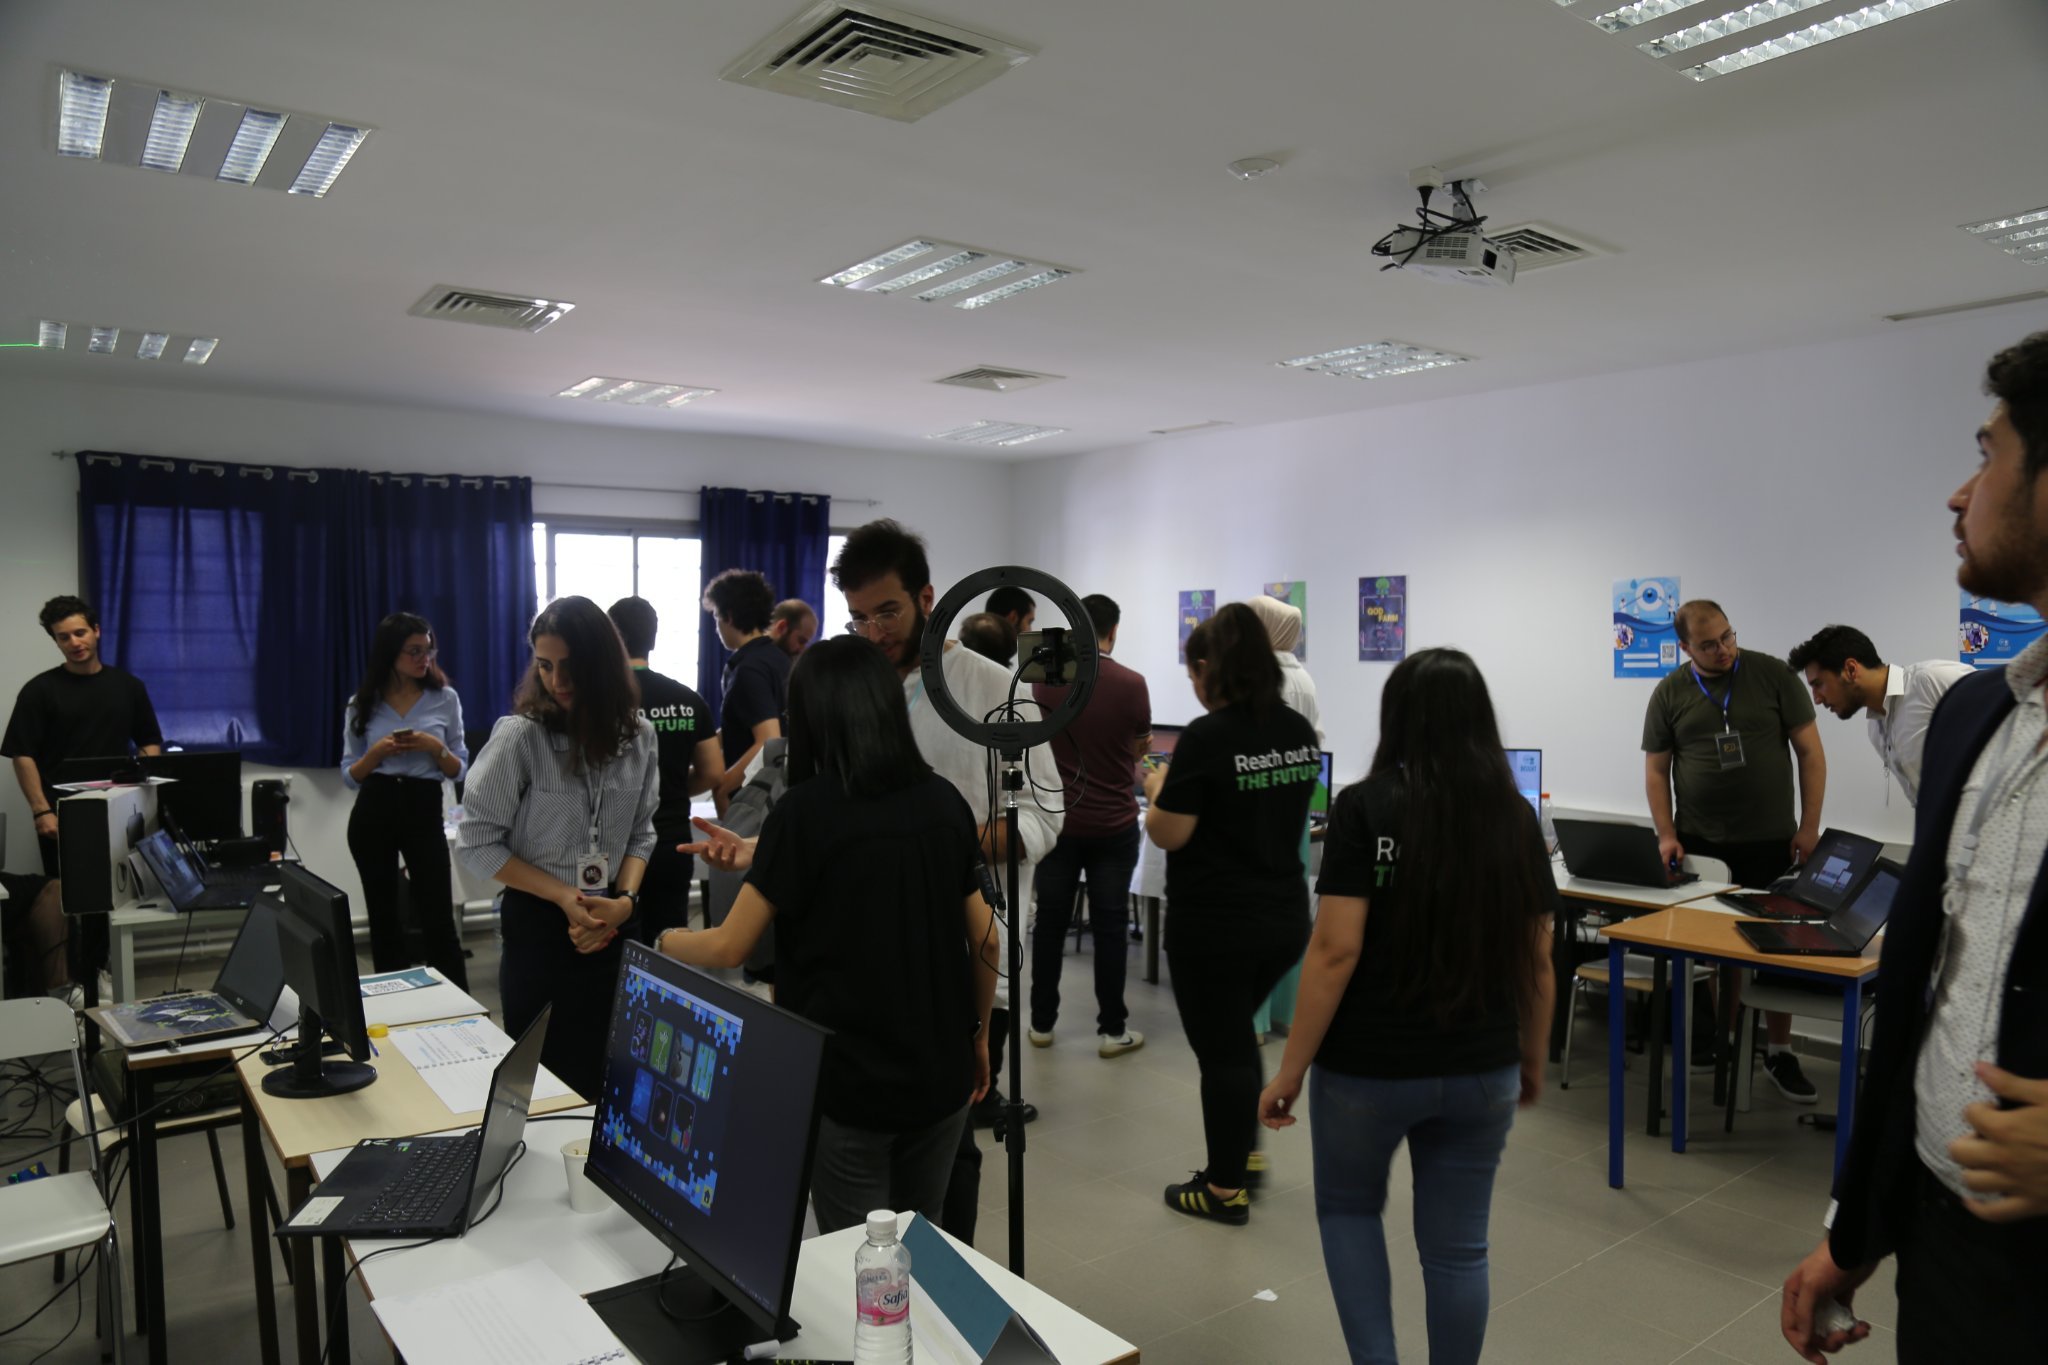
\includegraphics[scale=0.15]{event.jpg}
            \caption{One of the most famous events in esprit: bal des projets} 
            \label{fig: Student events exemple}
\end{figure}
Sometimes, it is very difficult for reserved and shy students to walk into a room full of unknown individuals. In addition, this approach is not guarantee of friendships of lasting significance as opposed to the case in a cultural setting like Tunisia where the norms may differ.
Regarding transport, we find that a majority of the bus service users or the demand that come from Tunisia are the school and university students, where in 2019 they represented 53\% of the entire population and are constantly on the rise. \cite{Share_of_students_in_total_bus_passengers}
\begin{figure}[H] 
            \centering
            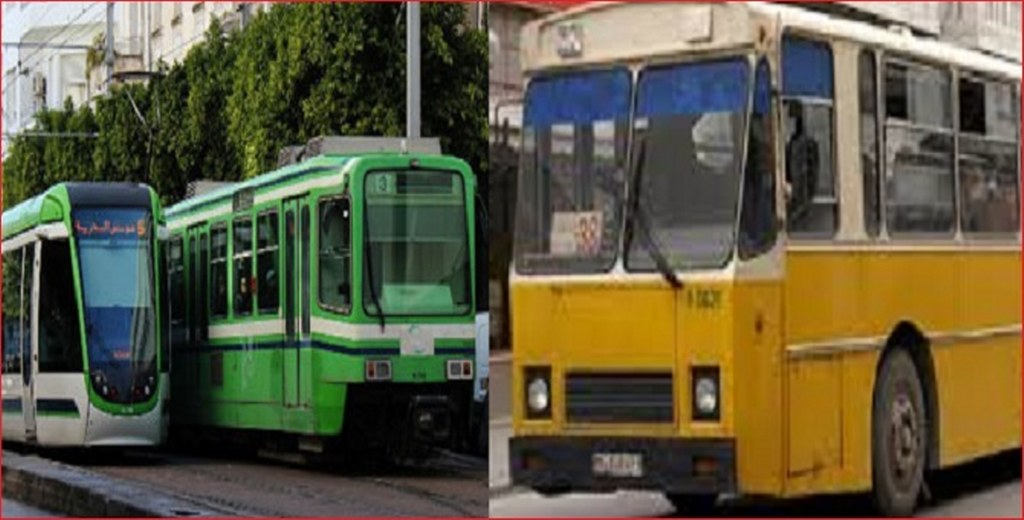
\includegraphics[scale=0.3]{bus-metro-tunis.jpeg}
            \caption{example of public means of transportation: bus and metro} 
            \label{fig: example of means of transportation}
\end{figure}
Even though, using public transport to get to university may be convenient and costs mere money, it has certain disadvantages:
\begin{itemize}
    \item lack of safety.
    \item very tiring
    \item time-consuming
    \item lack of comfort
\end{itemize}
To avoid that, some students use taxis, which offers comfort and fast service, but also has its drawbacks: 
\begin{itemize}
    \item taxis can be very expensive if they are a daily means of transport.
    \item taxis can be hard to find in some areas
    \item sometimes unavailable
\end{itemize}
\begin{figure}[H] 
            \centering
            \includegraphics[scale=0.2]{Taxis_in_Tunesien.jpg}
            \caption{example of means of transportation: Taxis} 
            \label{fig: example of means of transportation 2}
\end{figure}
Students in a rush usually opt for private cabs provided by apps, like Bolt and inDrive. All the same, such cabs have disadvantages and one of the biggest reasons students do not use them often is because most of them are not cost-effective or even affordable to some people.
\begin{figure}[H] 
            \centering
            
\includegraphics[scale=0.5]{apps_logo.png}
            \caption{example of Transportation applications: Bolt and inDrive} 
            \label{fig: example of Transportation apps}
\end{figure}

So, since not all existing solutions are suitable for students, how can we meet their needs?

\section{Proposed solution}
Though the above solutions may work for some, they have their own problems and limitations and cannot work for students overall, because students are very sensitive target. \\
That’s why uni-world thought of satisfying students’ needs by taking the drawbacks of all existing solutions and correcting them to give us the best solution for students. \\

Uni-world is divided into two modes: uni-match and uni-carpool.
\begin{itemize}
\item uni-match is a space for students to meet and make new friends in a safe, easy, and fun way, solving the problems of the usual dating apps.
\item uni-carpool is an environment for students looking for transportation and for those who want to earn money. uni-carpool enables students to find or create carpooling opportunities.
\end{itemize}


\section{Methodology process}

When designing an application as complex as Uni-World, which is best built to respond to users daily needs and frequently change, the project’s management structure must be equally fluid and adaptive. Therefore, this project opted for Agile methodology because it is flexible, and involves constant increment and enhancement processes. 
\subsection{Agile Methodology}
When it comes to projects, agile methodologies are perfect, and they are implemented when the requirements are not clearly outlined, or when the customers expect changes on the application. The basis for our work in the development of “Uni-world” We have decided to choose one of the currently popular methods, namely SCRUM.
Speaking about the methods of project management and taking into account such a great number of available methods, we have decided to use the SCRUM method for the development of the “Uni-World”. \\

\subsection{Chosen Methodology: Scrum}
The Scrum Method is one of the Agile frameworks that divides the developmental process into iterations that are time-bound and commonly known as sprints. The best practice in this development is called Scrum which entails various roles as well as artifacts that act as crucial events. \\ \\
Key Components of Scrum: 
\begin{itemize}
    \item Roles:
    \begin{itemize}
    \item Product Owner: Acts as a representative of the stakeholders and is charged with the responsibility of outlining and prioritizing of the product backlog.
    \item Scrum Master: Coaches in Scrum, enforces the use of Scrum practices, and dissolves impediments.
    \item Development Team: A team which is composed of members from different divisions and who is accountable for the delivery of the item of work for the product increment.
\end{itemize}
    \item Events:
    \begin{itemize}
    \item Sprint Planning: A process of planning what has to be achieved in the current sprint and which items from the product backlog should be developed.
    \item Daily Standup: Specifically, Scrum refers to a 15-minute daily communication, where the team reports to one another regarding the work completed, work to be done and possible obstacles.
    \item Sprint Review: A face-to-face or video conference near the end of the sprint during which the stakeholders are presented with the work that has been done and their input is taken.
\end{itemize}   
\item Artifacts:
\begin{itemize}
    \item Product Backlog: This denotes an arrangement of features, enhancements, and fixes essential for the product. Sprint Backlog: It is a list of tasks to be taken up during the sprint which is culled out from the product backlog.
    \item Increment: This is a precise or concrete product obtained at the end of every sprint.
\end{itemize}
\end{itemize}

\begin{figure}[H] 
            \centering
            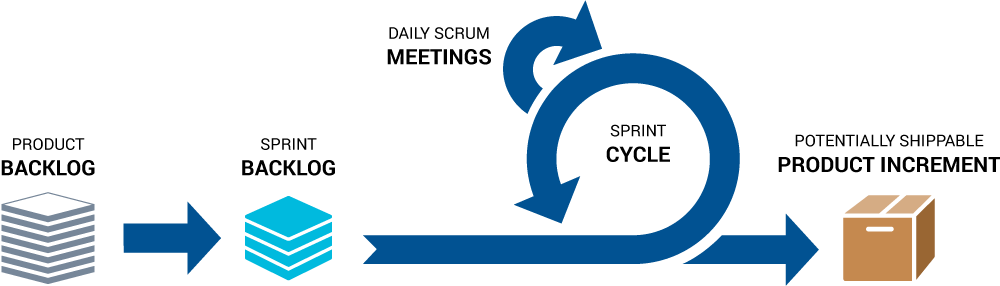
\includegraphics[scale=0.45]{agile.png}
            \caption{Agile Software Development Methodology SCRUM} 
            \label{fig: Agile Software Development Methodology SCRUM}
\end{figure}
\subsection{Why SCRUM ?}
We chose SCRUM because of its three-pillar foundation:We chose SCRUM because of its three-pillar foundation:
\begin{itemize}
    \item Inspection: again and again, Scrum tries to make it compulsory to assess differently. created to identify if there was any shift in their design towards the negative direction. These inspections should not be conducted in such a manner that it results in a negative impact on the health of citizens, the economy, or the environment.
    be carried out too frequently, or by a poorly-trained inspector: this would retard the project progress.
    \item Transparency: Communication is at the core of scrum since all the development activities are centered on a common language.
    \item Adaptation: This again means that when a deviation is noted during inspection the process must be halted.
\end{itemize}
\subsection{Scrum team structure}
As we have opted for a Scrum method, the role distribution will be as 
follows in the Table below:
\begin{table}[h]
    \centering
    \begin{tabular}{|p{3cm}|p{4cm}|p{8cm}|}
        \hline
        Role & Actor & Mission\\
        \hline
        Product Owner & Mouheb eddine saadaoui & Responsible for updating and managing the product backlog. \\
        \hline
        Scrum Master & Ahmed hchaichi & Responsible for establishing Scrum and team efficiency. \\
        \hline
        Scrum Team & Bairem khedhri & Responsible for the development of the product \\
        \hline
    \end{tabular}
    \caption{Text description of the carpooling offer management use case}
    \label{Tab: Text description of the carpooling offer management use case}
\end{table}


\section*{Conclusion}
In this first chapter, we discussed the project as a whole. First, we took a look at the general context of the project to understand the project in a nutshell, then moved on to the presentation of the hosting company. Following this, we saw the problem and how the students were struggling, we had a look at the existing solutions and critiqued them to see their shortcomings and how to remedy them, and finally, we presented the methodology we are adopting in the project. In the next chapter, we'll look at the functional and technical aspects of the application.

 
  
\chapter{Preliminary Analysis}\label{chapter:PA}


\section*{Introduction}
\addcontentsline{toc}{section}{Introduction}
Following that, having reviewed the theoretical concepts that will help to improve the understanding of the project, we proceed to the requirements analysis and technical specifications stage. In this second chapter, we construct the functional study of the project and minor sequence diagrams of use case and technical study of the technologies used in the project.

\section{Functional study}
The functional study is a crucial step in the process of understanding the subject and the activities that will be performed. It normally features the actors, the functional responsibilities of these actors and the dynamic between the different actors in the form of UML diagrams.

\subsection{Identifying the system actor}


The key actor in Uni-world is the \textbf{Student}, who will benefit from the application's functionalities. \\
The application will only permit students to use it by providing additional authentication details such as submitting a university e-mail address, the form of which is well specified.

\subsection{Identifying functional requirements}
\textbf{Functional requirements represent the features provided by the system to meet the user's expectations, listing the key functionalities that uni-world offers:}\\
The application comprises the following modules : 
\begin{itemize}
    \item User Management Module:\\
The User Management Module covers the application of the actual management of the users. An example of it is password login, user registration, activation of an account, password reset, and other details about the account. This module provides users with as much simplicity and security as possible while signing up or logging in to the service.
\begin{itemize}
\item Login: \\
Confirm the validity of the student by entering the university and password that is set by the student.
\item Registration: \\
Easy registration form with input values including name, e-mail address ,password and other data that are useful to build the user profile.
E-mail address verification is used to confirm the existence of an account and prevent spam. It can also be used to determine the authenticity of the user and his or her university.
\item Account Activation:\\
As for the link activation of new users, the emails will be sent.
Short accountability of account activation related to increased brand recognition.
\item Password Reset:\\
Password change mechanism over email using a trusted link.
User confirmation or the extra dilemma in changing the password to enhance security features.
\item Account Management:\\
Menu entries can be used to input new personal details of the user, to change passwords, and to set the level of privacy.
\end{itemize}    
    \item Profile Swiping Module:\\
This specific learning module is to encourage students to make friends and interact with each other through a feature of swiping cards like the Bumble application. This is useful to help a student, for example, if they want to meet new people or if they do not want to interact with people, this feature allows it.
\begin{itemize}
\item Profile Creation: \\
We can keep identity information by making personal and unique profiles with profile pictures, about oneself details, and more.
\item Swiping Mechanism: \\
Like the real world, the app or site allows you to ‘swipe right’ to indicate you are interested and ‘swipe left’ to show the opposite.
Inclusion of algorithms through which the application can identify the list of profiles with, which the user is likely to share a common interest and/or mutual friends.
\item Matching: \\
Students tap on each other’s picture to match once two students have swiped right, they are matched.
An alert message is sent to the two users regarding the match.
\item Chat Initiation: \\
Matched users have the privilege of chatting each other somewhere within the App.
End-to-end also means having a secure and private chat environment.
\end{itemize}
\item Carpooling Module: \\
Finding ways how to get to school without hiring personal transport is a key concern amongst students, this module caters to that aspect as students will find means to share transport costs.\\
\begin{itemize}
\item Creating Carpool Offers: \\
Carpool offers can be offered and posted by the users; with additional information such as the destination, time, and number of seats available among others.
\item Browsing Carpool Offers: \\
This way the students can see all the Carpool offers present in their vicinity.
There are various fields to filter its searches so that their offers will meet their desired time schedule and preferred location.
\item Expressing Interest: \\
It means showing interest in carpool offer by swiping right hand side.
If a user does not want to claim an offer, he can just swipe left on the page.
\item Offer Acceptance: \\
Interests of users are promptly alerted to the offer owners.
Owners are also able to view all the interest requests that are made to them, and they have the privilege of either approving or rejecting them.
An alert message is sent to the two users regarding the match.
\item Chat for Carpool Coordination: \\
After an acceptance, there starts a chat between the owner of the carpool offer and the intended user.
Is useful in co-coordinating and sealing all the details of a carpool and other related matters.
\end{itemize}
    \item Notifications Module: \\
The Notifications Module makes sure that the user will always be notified on activities and updates that are taking place within the application.
    \begin{itemize}
    \item Real-time Notifications: \\
Notifications of new messages, date arrivals, people interested in carpooling etc.
\item Customizable Notification Settings: \\
They are able to do this under the application settings tab where they have the ability to turn off notifications from the application.
    \end{itemize}
\end{itemize}

\subsection{Identifying non-functional requirements}
Nevertheless, non-business requirements are not related to business directly. however, this aspect must be included in the requirements definition to achieve better application quality. Our solution must ensure for our solution to be effective it must meet the following :
\begin{itemize}
    \item Maintainability: or in other words, the level to which an application is known or fixed or enhanced in a way to pose no challenge to the new developers working on the application in terms of code readability and implementation and this is achieved by proper documentation of the code and good comments placed at relevant places in the code and place appropriate names for the class, variables and methods used in the application.
    \item Usability: the application must be easily manipulable and has clean, updated high and fluid interaction and suited for both small screen mobile and larger screen and bigger. This is made possible given that the jetpack compose improves the making of interfaces that are easy to use together with a swipe system.
    \item Extensibility: Thus, the application is more versatile in terms of it possibility to be developed and implemented and containing more features due to its good initial setup resulting from the usage of design patterns and proper extendable architecture.
    \item Security: the application must be secure and access should be provided through the user rights only. JSON web token can also ensure the authenticity of the user hence reducing on invasions that can be conducted by other unlawful users, The passwords and the messages are also encrypted hence ensuring the user confidentiality.
\end{itemize}


\subsection{ Global Use case diagram}
The use case diagram describes the system's behavior from the user's point of view. It divides its functionalities into use cases that express the needs of its users, as shown in Figure 2.1 below.

\begin{figure}[H] 
            \centering
            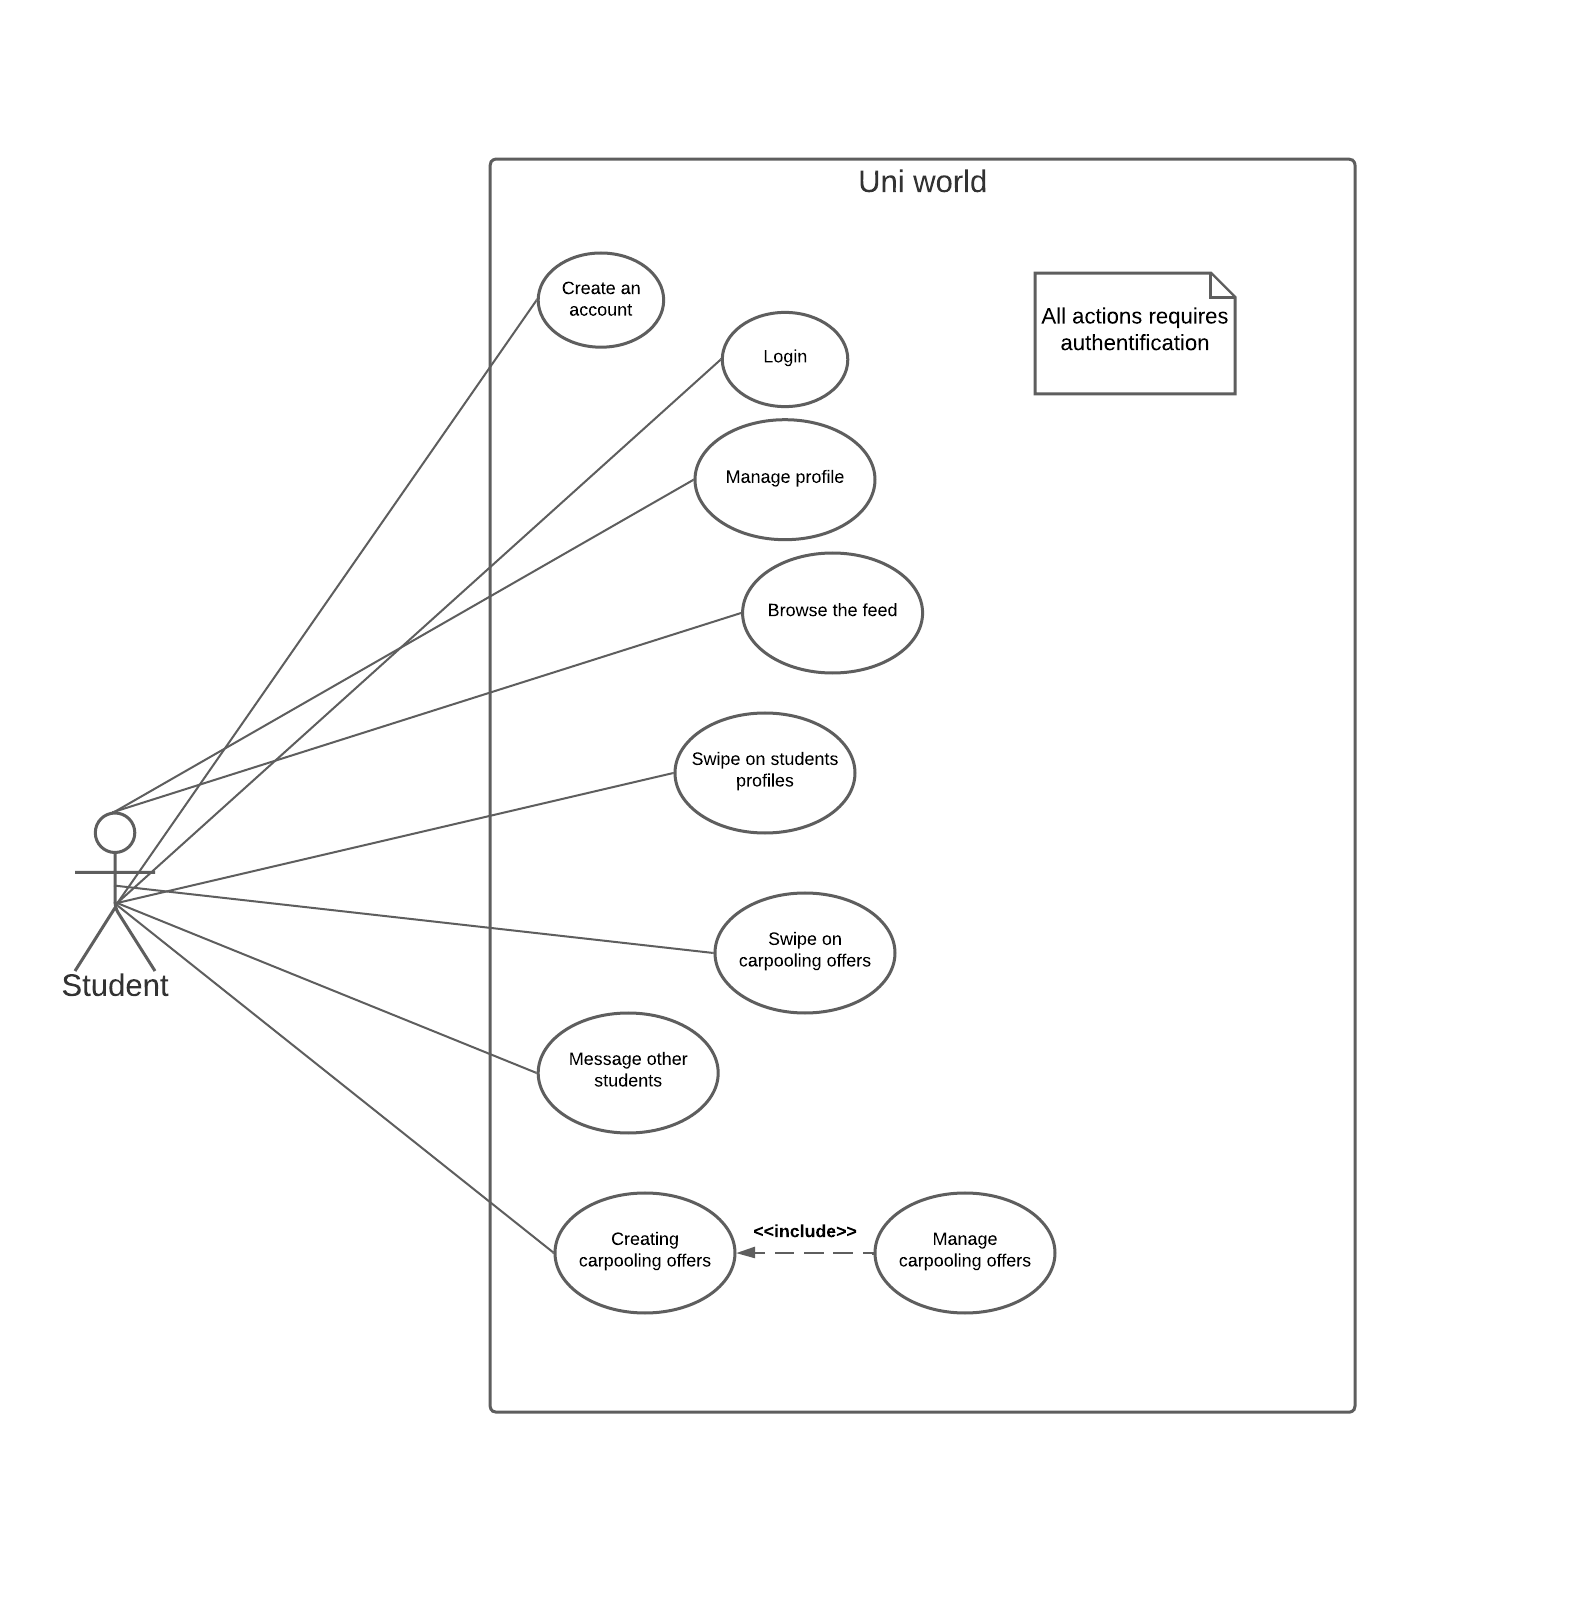
\includegraphics[scale=0.5]{diagrams/global use case.png}
            \caption{Global use case diagram} 
            \label{fig: Global use case diagram}
\end{figure}
\space
\section{Project management using Scrum}
Referring to Chapter 1, page 16, subsection 1.6.3, it is discussed that the Project is managed according to SCRUM methodology because of its efficiency and application to the project.

\subsection{Product backlog}

The Product Backlog is the working document of the project that contains all the anticipated functionalities.
of the product that is used often, these are commonly known as user stories.
that all residues related to the products lies with the priority of the Product Owner
the User Stories of the Product Backlog using the MoSCoW method:the User Stories of the Product Backlog using the MoSCoW method:
\begin{itemize}
    \item M (Must Have) : it stands for what needs to be done. It is important to conclude this criterion to fully meet project objectives. They classified it as high criticality.
    \item S (Should Have) : This is a must adjustment that must be made whenever possible. If not, it can be done later so as to fit the time line of the project.
    \item C (Could Have) : This is a need that is highly desirable but, unlike the essential needs, can be satisfied without having much effect on the rest of the tasks in the day.
    \item W (Won’t have) : It is optional to implement, but would be an interesting nice to have, though not a must
\end{itemize}
The Product backlog for this project is shown in the table below:

\begin{table}[H]
    \centering
    \begin{tabular}{|p{0.5cm}|p{12cm}|p{2cm}|}
        \hline
ID & User Story & Priority \\
\hline
1 & As a student, I want to register easily and securely & M \\
\hline
2 & As a student, I want to log in to a space reserved for students & M \\
\hline
3 & As a student, I want to show my interest by swiping right on someone so that I can contact them if they like me back & M \\
\hline
4 & As a student, I want to ignore someone I don't find interesting & M \\
\hline
5 & As a student, I want to receive an email to activate my account & C \\
\hline
6 & As a student, I want to receive an email to change my password if I have forgotten it & M \\
\hline
7 & As a student, I want to send and receive messages from my matches & M \\
\hline
8 & As a student, I want to see who likes me so I can decide whether or not to like them back & S \\
\hline
9 & As a student, I want to filter my feed according to many criteria & S \\
\hline
10 & As a student, I want to choose the gender I want to interact with & C \\
\hline
11 & As a student, I want to change my password & M \\
\hline
12 & As a student, I want to switch from social mode to carpool search mode & M \\
\hline
13 & As a student, I want to browse available carpooling offers & M \\
\hline
14 & As a student, I want to show my interest if I find an offer interesting, and ignore offers I don't like & M \\
\hline
15 & As a student, I want to create a carpool offer & M \\
\hline
16 & As a student, I want to manage my carpool offers & M \\
\hline
17 & As a student, I want to see who's interested in my offers & M \\
\hline
18 & As a student, I want to accept or reject other users interested in my offers & M \\
\hline
19 & As a student, I want to receive notifications when I get a match or message & S \\
\hline
20 & As a student, I want to manage my account & M \\
\hline
    \end{tabular}
    \caption{Product backlog}
    \label{Tab: Product backlog}
\end{table}
\subsection{Sprint Planning}
The table below shows the breakdown of the project into user stories for each sprint :
\begin{table}[H]
    \centering
    \begin{tabular}{|p{2cm}|p{6cm}|p{4cm}|}
        \hline
Sprint ID & Title & User Stories \\
\hline
1 & User management & 1-2-5-6-11-20 \\
\hline
2 & Social life features (Uni-match) & 3-4-7-8-9-10 \\
\hline
3 & Carpooling features (Uni-car) & 12-13-14-15-16-17-18-19 \\
\hline
    \end{tabular}
    \caption{Sprint Planning}
    \label{Tab: Sprint Planning}
\end{table}
\section{Class diagram}
As will be seen in the following sections, it is useful to prepare a class diagram to understand each component of this application in detail. This diagram shows all classes which include their attributes and methods and also relations between classes. \\
It becomes important to have this form of presentation to easily comprehend the code’s architecture. This allows the developers to see how the varied parts relate to each other and how they are interconnected, especially in the designing and development phase.

\begin{figure}[H] 
            \centering
            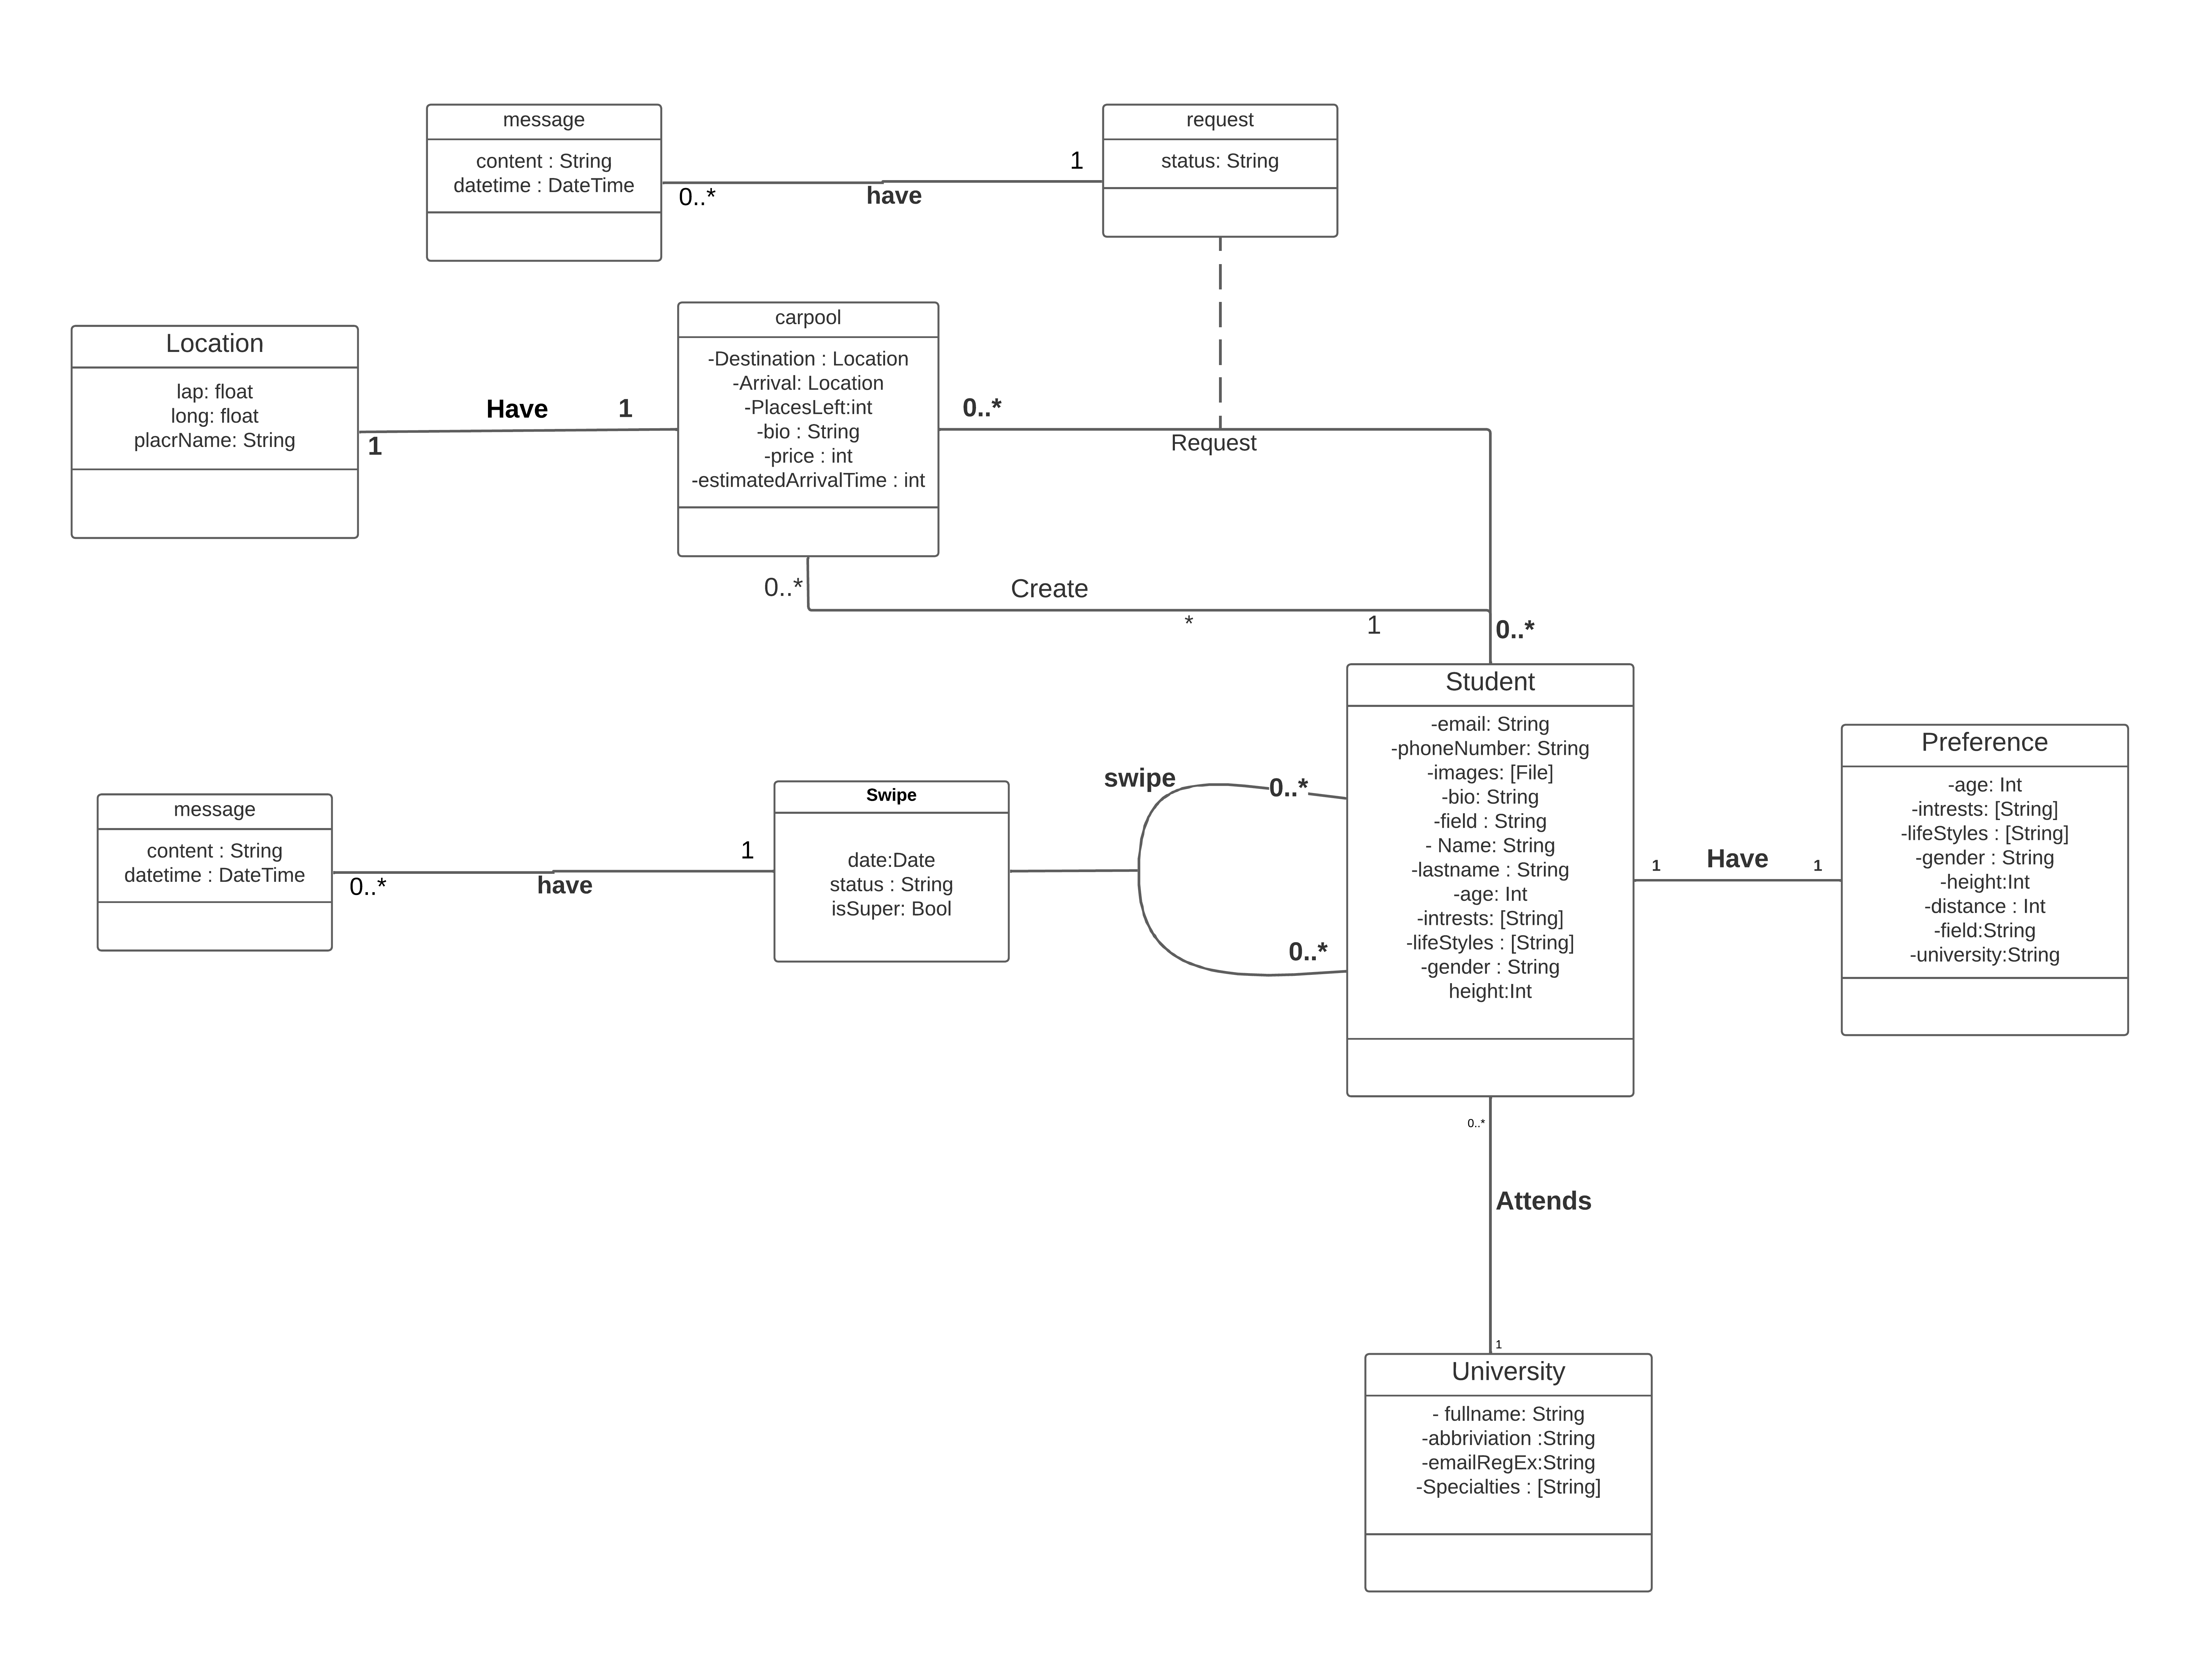
\includegraphics[scale=0.3]{diagrams/class diagram.png}
            \caption{Uni-world's class diagram } 
            \label{fig: Uniworld's class diagram}
\end{figure}

\section{Uni-world architectural conception}
\subsection{Physical architecture}
The physical architecture of our solution requires a hardware infrastructure to guarantee efficient operation of the application. A powerful, reliable server is crucial. For Uni-world, we opted for an N-tier architecture.
Consequently, Uni-world will be structured around three main Tiers, Presentation Tier, Application Tier and the data Tier, each playing a distinct role:
\begin{itemize}
    \item Presentation Tier (Jetpack compose): this layer supports the user interface and experience
    experience on mobile devices. Using the Jetpack compose Framework, it enables you to
    create an intuitive, responsive interface, providing a smooth, seamless user
    experience.
    \item Application Tier (Node .js): this layer is the “brain” of our application, in charge of all business logic and data processing. It is crucial to guarantee the application's performance, security and scalability.
    \item Data Tier (MongoDB): this layer manages and stores the data.
    data. It must guarantee the integrity, consistency and availability of information.
\end{itemize}
\begin{figure}[H] 
            \centering
            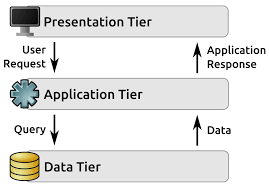
\includegraphics[scale=0.9]{physical archi.png}
            \caption{N-Tier Physical architecture} 
            \label{fig: N-Tier Physical architecture}
\end{figure}
\subsection{Software architecture}
Software architecture refers to the structures that are required for comprehending a software system while also constituting the practice of designing such structures and systems. Every structure is better described as software entities, interconnections between the entities, and attributes of both entities and relations. \\
In this application, we have adopted the CLEAN architecture and MVVM architectural pattern for the presentation section as outlined in the following figure.

\begin{figure}[H] 
            \centering
            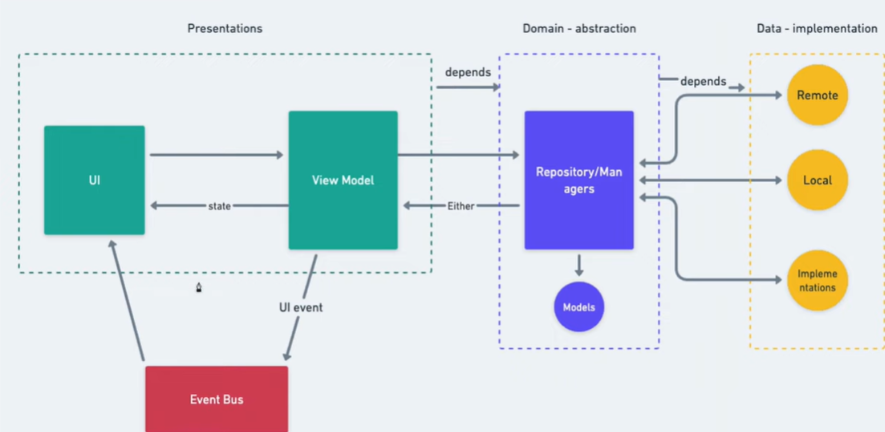
\includegraphics[scale=0.8]{mvm.png}
            \caption{Software architecture : CLEAN architecture and MVVM } 
            \label{fig: CLEAN architecture and MVVM}
\end{figure}

\section{Hardware resources}
The table 2.3 shows the hardware setup used in our project.
\begin{table}[H]
    \centering
    \begin{tabular}{|p{4cm}|p{6cm}|}
        \hline
        Owner & Bairem khedhri\\
        \hline
        RAM & 16,0 GB \\
        \hline
        CPU & 11th Gen Intel(R) Core(TM) i5-11400H @ 2.70GHz   2.69 GHz \\
        \hline
        Storage & 512 Go SSD \\
        \hline
        Operating system  & Windows 11 Professional 64-bit \\
        \hline
    \end{tabular}
    \caption{Hardware resources}
    \label{Tab: Hardware resources}
\end{table}

\section{Work environment}
For a project as heavy as uni-world, I need several tools and software to help me improve the project, such as : \\
\begin{itemize}
    \item \textbf{Figma:} A tool used in the development of the application, particularly in the UX/UI 
    design where the application is designed and a prototype made.
        \begin{figure}[H] 
            \centering
            
\includegraphics[scale=0.03]{logos/Figma-logo.png}
            \caption{Figma logo } 
            \label{fig: Figma logo}
        \end{figure}
    \item \textbf{Github:} is a software development platform which enables developers to 
    build, host and collaborate on code. This one integrates git software, which adds distributed 
    version control of Git plus, access control, bug tracking, Software requests features, task management, continuous integration, and wikis for every project.
        \begin{figure}[H] 
            \centering
            
\includegraphics[scale=0.15]{logos/github-logo.png}
            \caption{Github logo } 
            \label{fig: Github logo}
        \end{figure}
    \item \textbf{Lucidchart:} A fully managed cloud based tool to create diagrams, data visualization and concept maps. It also offers users powerful features for modeling sophisticated information in a very easy and graphical manner.
        \begin{figure}[H] 
            \centering
            
\includegraphics[scale=0.2]{logos/lucichart-logo.png}
            \caption{Lucidchart logo } 
            \label{fig: Lucidchart logo}
        \end{figure}
    \item \textbf{Android Studio:} Is the integrated development environment or IDE is specifically for developing android applications. It provides a full and optimised environment for the development of applications for the Android system.
            \begin{figure}[H] 
                \centering
                
\includegraphics[scale=0.2]{logos/android-studio-logo.png}
                \caption{Android Studio logo } 
                \label{fig: Android Studio logo}
            \end{figure}    
    \item \textbf{Visual studio Code:} is this cross-platform code editor developed by Microsoft for MacOS, Windows and Linux operating systems, 
    it support native for many popular programming languages.
            \begin{figure}[H] 
                \centering
                
\includegraphics[scale=0.07]{logos/visual-studio-code-logo.png}
                \caption{Visual studio Code logo } 
                \label{fig: Visual studio Code logo}
            \end{figure} 
    \item \textbf{Postman:} This tool is one of the preferred to deal with RESTful API. It is a tool that enables and simplifies the launching, evaluating and the quick use of http requests for efficiency.
        \begin{figure}[H] 
            \centering
            
\includegraphics[scale=0.2]{logos/postman-logo.png}
            \caption{Postman logo} 
            \label{fig: Postman logo}
        \end{figure}
\end{itemize}
\section{Languages and Frameworks}
\begin{itemize}
    \item \textbf{Kotlin:} Is a statically typed, high-level programming language that can be used practically anywhere. Mostly know for its Android development and API creation.
        \begin{figure}[H] 
            \centering
            
\includegraphics[scale=0.04]{logos/kotlin-logo.png}
            \caption{Kotlin logo } 
            \label{fig: Kotlin logo}
        \end{figure}
    \item \textbf{Jetpack Compose:} Is a modern UI toolkit for Android that makes apps more intuitive with less code, easier maintainability and better runtime performance. It makes it easy to build an one-layer of view in your app with less code,compitable and intergrated well into other Jetpack libraries,makes all short work dynamic UI updates according to data changes.
        \begin{figure}[H] 
            \centering
            
\includegraphics[scale=0.06]{logos/jetpack-compose-logo.png}
            \caption{Jetpack Compose logo } 
            \label{fig: Jetpack Compose logo}
        \end{figure}
    \item \textbf{Javascript:} Is an object oriented-structured and a high level programming language which finds its applicability mainly in the creation of Web pages. It allows the dynamic content of the websites, forms validations, and control of multimedia objects. Born initially as a 
    client-side scripting language, JavaScript has evolved to be an essential technology in web development that operates both on the client and server-side for the development of interactive applications based on html and CSS.
        \begin{figure}[H] 
            \centering
            
\includegraphics[scale=0.2]{logos/javascript-logo.png}
            \caption{Javascript logo } 
            \label{fig: Javascript logo}
        \end{figure}
    \item \textbf{Node JS:} Is a runtime environment, it provides the environment of executing JavaScript on server side. Being constructed on Chrome’s V8 JavaScript engine, it is beneficial for creating applications with high efficiency and scalability. 
    Node. js is superb in dealing with the asynchronous events and real time data; this makes it a perfect choice in Web applications, APIs, and micro services.
            \begin{figure}[H] 
                \centering
                
\includegraphics[scale=0.5]{logos/node-logo.png}
                \caption{Node JS logo } 
                \label{fig: Node JS logo}
            \end{figure}    
    \item \textbf{MongoDB:} Is a NoSQL DBMS and is regarded as flexible and highly scalable. Data is stored in JSON-like documents and it offers therefore excellent flexibility regarding changing structures of the saved data. MongoDB is perfect for today’s applications because it provides superior querying and indexing functionality alongside the capacity to manage massive amounts of unstructured or semi-structured data.
            \begin{figure}[H] 
                \centering
                
\includegraphics[scale=0.3]{logos/mongo-logo.png}
                \caption{MongoDB logo } 
                \label{fig: MongoDB logo}
            \end{figure} 
        \end{figure}
\end{itemize}

\section*{Conclusion}
After the requirements specification analysis, the conceptual study and the new hardware and software environment for “uni-world”, we are in Sprints development for the progressive incarnation of our project in Sprints.
\chapter{Sprint 1: Authentication and User management}



\section*{Introduction}

\addcontentsline{toc}{section}{Introduction}

Considering the product backlog, and having planned the execution of the project for a course of three sprints, we focus on the first sprint. The sprint aims at setting up the skeleton of the project and the implementation of safe authentication and user management.

\section{Sprint Backlog}
To start, we outline the work to be done in this sprint. The schedule for this iteration
involves the user stories described in the following Table 3.1:

\begin{longtable}{|l|p{6cm}|p{8cm}|}
\hline
Sprint & User story & Task\\
\hline
\multicolumn{3}{|c|}{Initializing the project structure} \\
\hline
\endfirsthead

\multicolumn{3}{c}{{\bfseries}} \\
\hline
Sprint & User story & Task\\
\hline
\endhead

\hline \multicolumn{3}{|r|}{{Continued on next page}} \\ \hline
\endfoot

\hline
\endlastfoot

1 & As a student, I want to register easily and securely & \begin{itemize}
    \item Create the user model
    \item Create user registering feature on the server-side
    \item Create user registering interfaces
    \item Integration and testing
\end{itemize} \\ \hline

2 & As a student, I want to log in to a space reserved for students & \begin{itemize}
    \item Create login feature using web tokens
    \item Create user login interfaces
    \item Integration and testing
\end{itemize} \\ \hline

20 & As a student, I want to manage my account & \begin{itemize}
    \item Create user profile management features on the server side
    \item Create profile management interfaces
    \item Integration and testing
\end{itemize} \\ \hline

6 & As a student, I want to receive an email to change my password if I have forgotten it & \begin{itemize}
    \item Integrate emailing feature in server-side using Node Mailer
    \item Create forget password Interfaces
    \item Integration and testing
\end{itemize} \\ \hline

11 & As a student, I want to change my password & \begin{itemize}
    \item Create changing password feature in the backend
    \item Create changing password interfaces
    \item Integration and testing
\end{itemize} \\ \hline

5 & As a student, I want to receive an email to activate my account & \begin{itemize}
    \item Create user account activation features on the server side
    \item Create account activation interfaces
    \item Integration and testing
\end{itemize} \\ \hline
\caption{Sprint 1 backlog}
\label{Tab: Sprint 1 backlog}
\end{longtable}


\section{ Analysis and conception}
In this section, we illustrate the sprint analysis in a more visual representation using use case diagrams and sequence diagrams of the most highlighted features:
"Login" and "Signup".

\subsection{Use case diagrams}
More detail on the “login” use case can be found in figure 3.1 that rounds up the diagram of the use case.

\begin{figure}[H] 
            \centering
            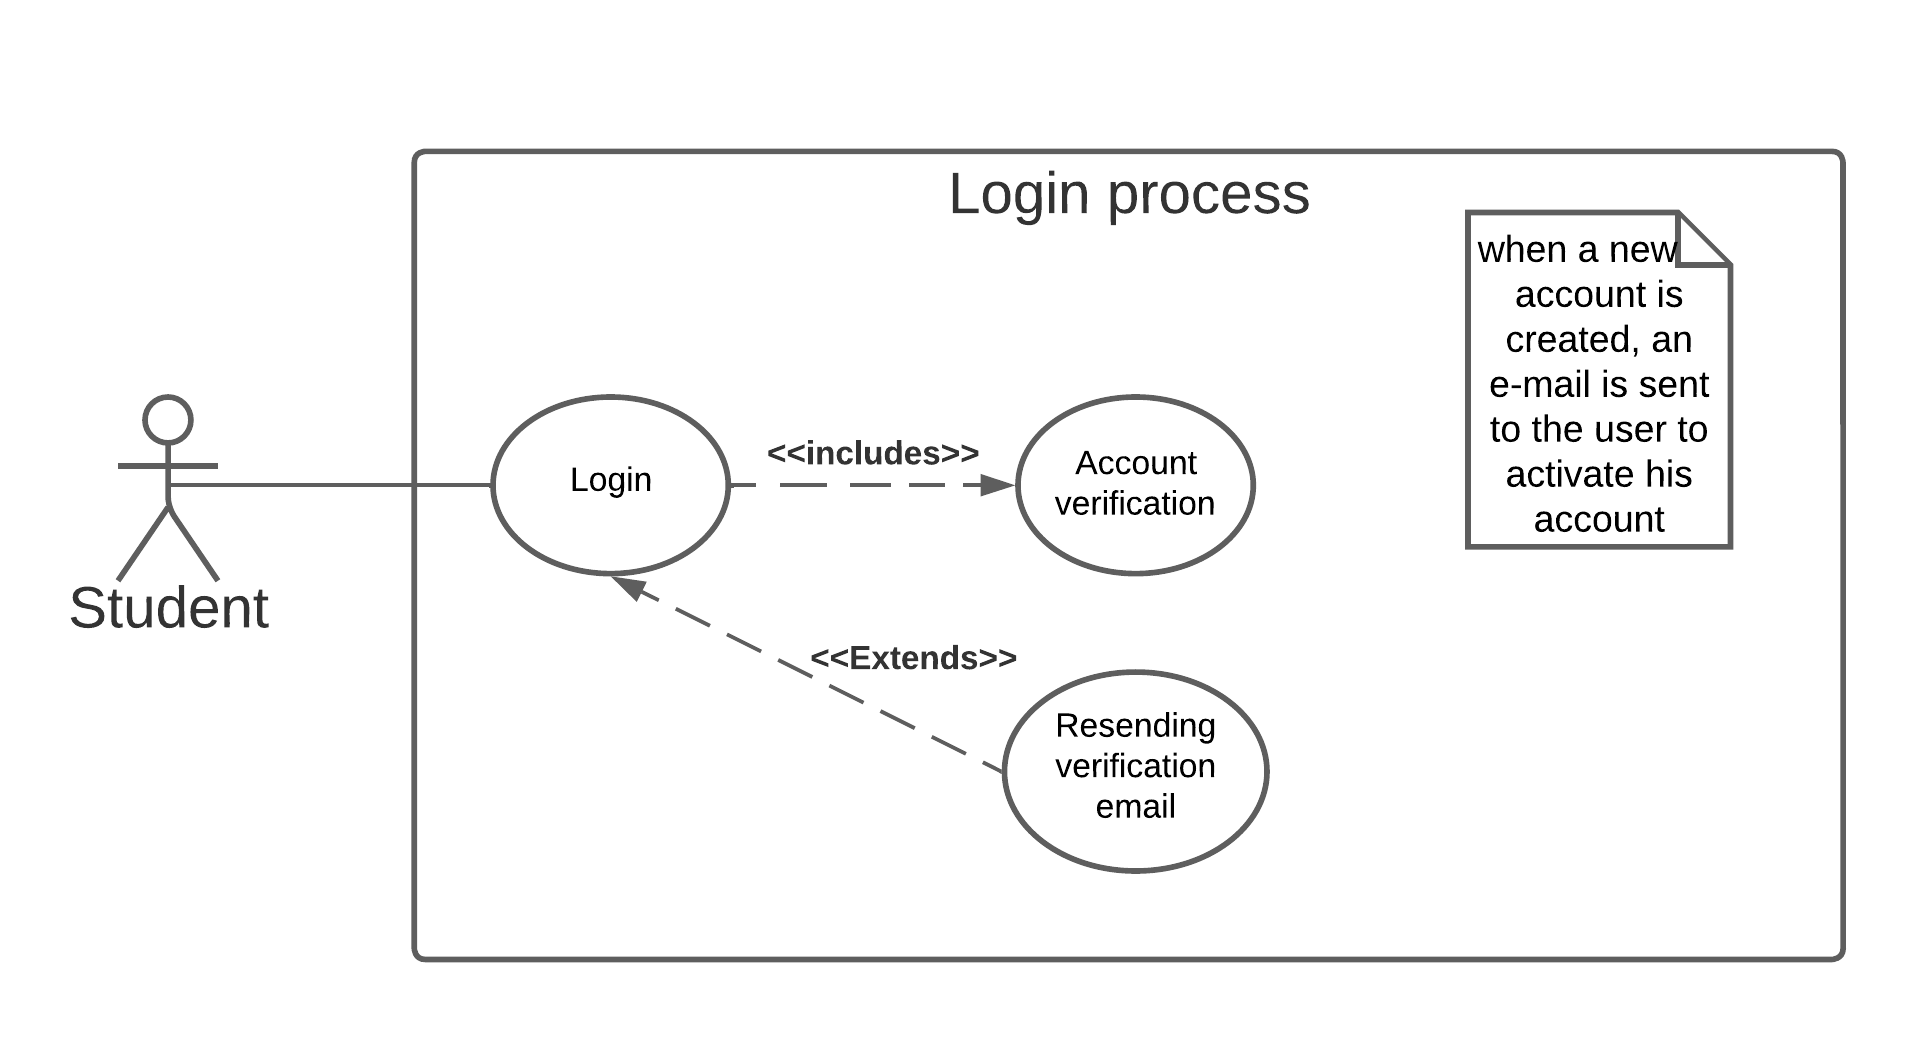
\includegraphics[scale=0.9]{diagrams/refined use case login.png}
            \caption{Login use case diagram} 
            \label{fig: Login use case diagram}
\end{figure}

The diagram of the "Signup" use case is shown in figure 3.2 :

\begin{figure}[H] 
            \centering
            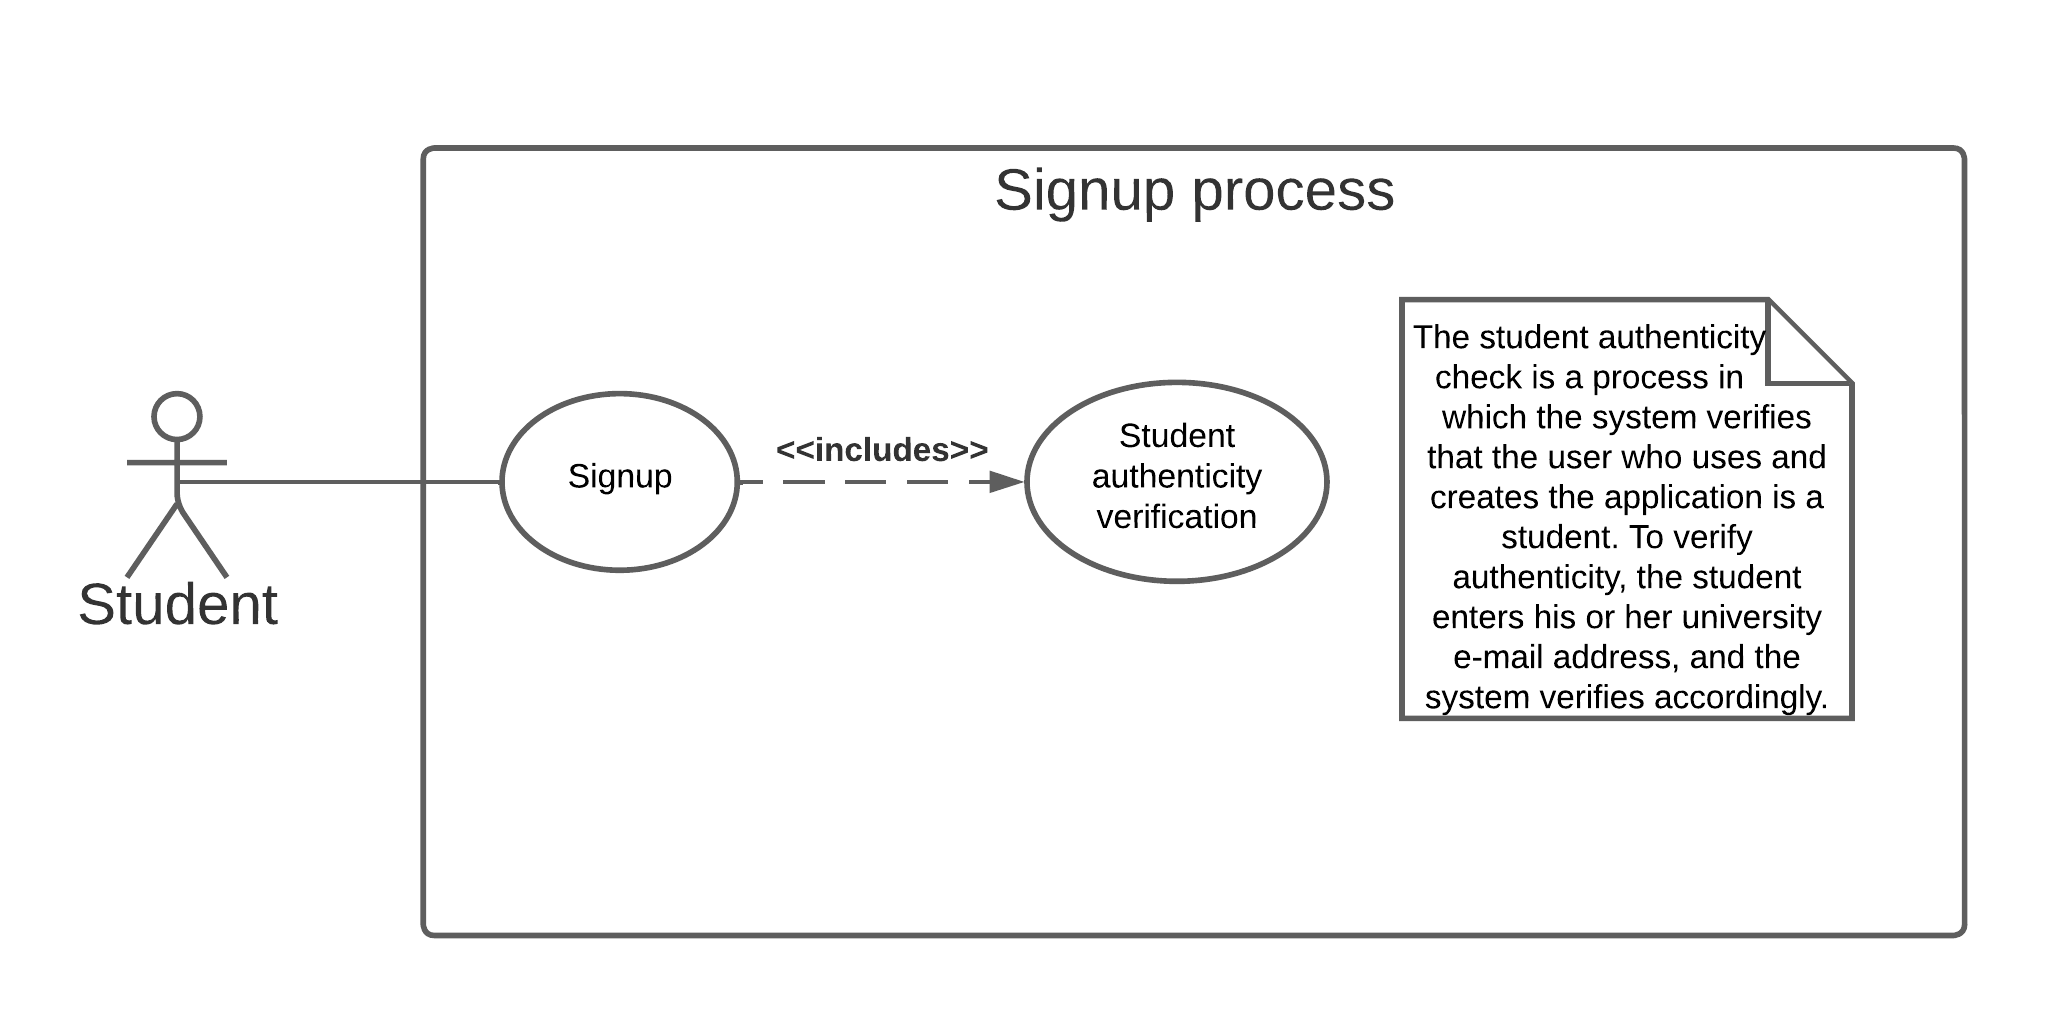
\includegraphics[scale=0.9]{diagrams/refined use case signup.png}
            \caption{signup use case diagram} 
            \label{fig: signup use case diagram}
\end{figure}

\subsection{Use case textual descriptions}
Textual descriptions of the "Login" use case are illustrated in table 3.2 below:
\begin{longtable}{|c|p{10cm}|}
\hline
Use Case & Description \\\hline
Name & Login use case \\\hline
Preconditions & The student's account must be active \\\hline
Postconditions & The student is logged in to a student-only space \\ \hline
Main Flow & \begin{enumerate}
    \item The user puts his coordinates(email and password) 
    \item The system checks if the account is activated or not
    \begin{enumerate}
        \item if the account is activated the user login successfully 
        \item if the account is not activated, the system shows an error message
    \end{enumerate}    
\end{enumerate}
\\\hline
Alternative Flows & \begin{itemize}
    \item if the user is not found, an error message appears
    \item if the user wrote bad credentials, an error message appears
    \item if there is a network error, an error message appears
\end{itemize}
\\\hline
Non-functional Requirements & \begin{itemize}
    \item The login will be secured thanks to the JSON Web tokens
    \item The login will be easy and the user will be aware of any problems
\end{itemize}
\\\hline
\caption{Textual descriptions of the Login use case}
\label{Tab: Textual descriptions of the Login use case}
\end{longtable}

The use case textual descriptions of "Signup" is illustrated in the
following Table 3.3:

\begin{longtable}{|c|p{10cm}|}
\hline
Use Case & Description \\\hline
Name & Signup use case \\\hline
Preconditions & The user must be a student \\\hline
Postconditions & A new account is created and an activation email is sent \\ \hline
Main Flow & \begin{enumerate}
    \item The user puts his university and email so the system can determine if he's a student of that university or not
    \item The user puts his additional information(name , last name , birthday , ...) 
    \item The user puts his pictures and they must be authentic 
    \begin{enumerate}
        \item if one of the information is unacceptable or empty the system shows an error message
        \item if the provided information is acceptable, the account will be created
    \end{enumerate}    
\end{enumerate}
\\\hline
Alternative Flows & \begin{itemize}
    \item if the user is not found, an error message appears
    \item if the user wrote bad credentials, an error message appears
    \item if there is a network error, an error message appears
\end{itemize}
\\\hline
Non-functional Requirements & \begin{itemize}
    \item The login will be secured thanks to the JSON Web tokens
    \item The login will be easy and the user will be aware of any problems
\end{itemize}
\\\hline
\caption{Textual descriptions of the Signup use case}
\label{Tab: Textual descriptions of the Signup use case}
\end{longtable}

\subsection{Sequences diagram}
The login sequence diagram can be observed in Figure 3.3 below:

\begin{figure}[H] 
            \centering
            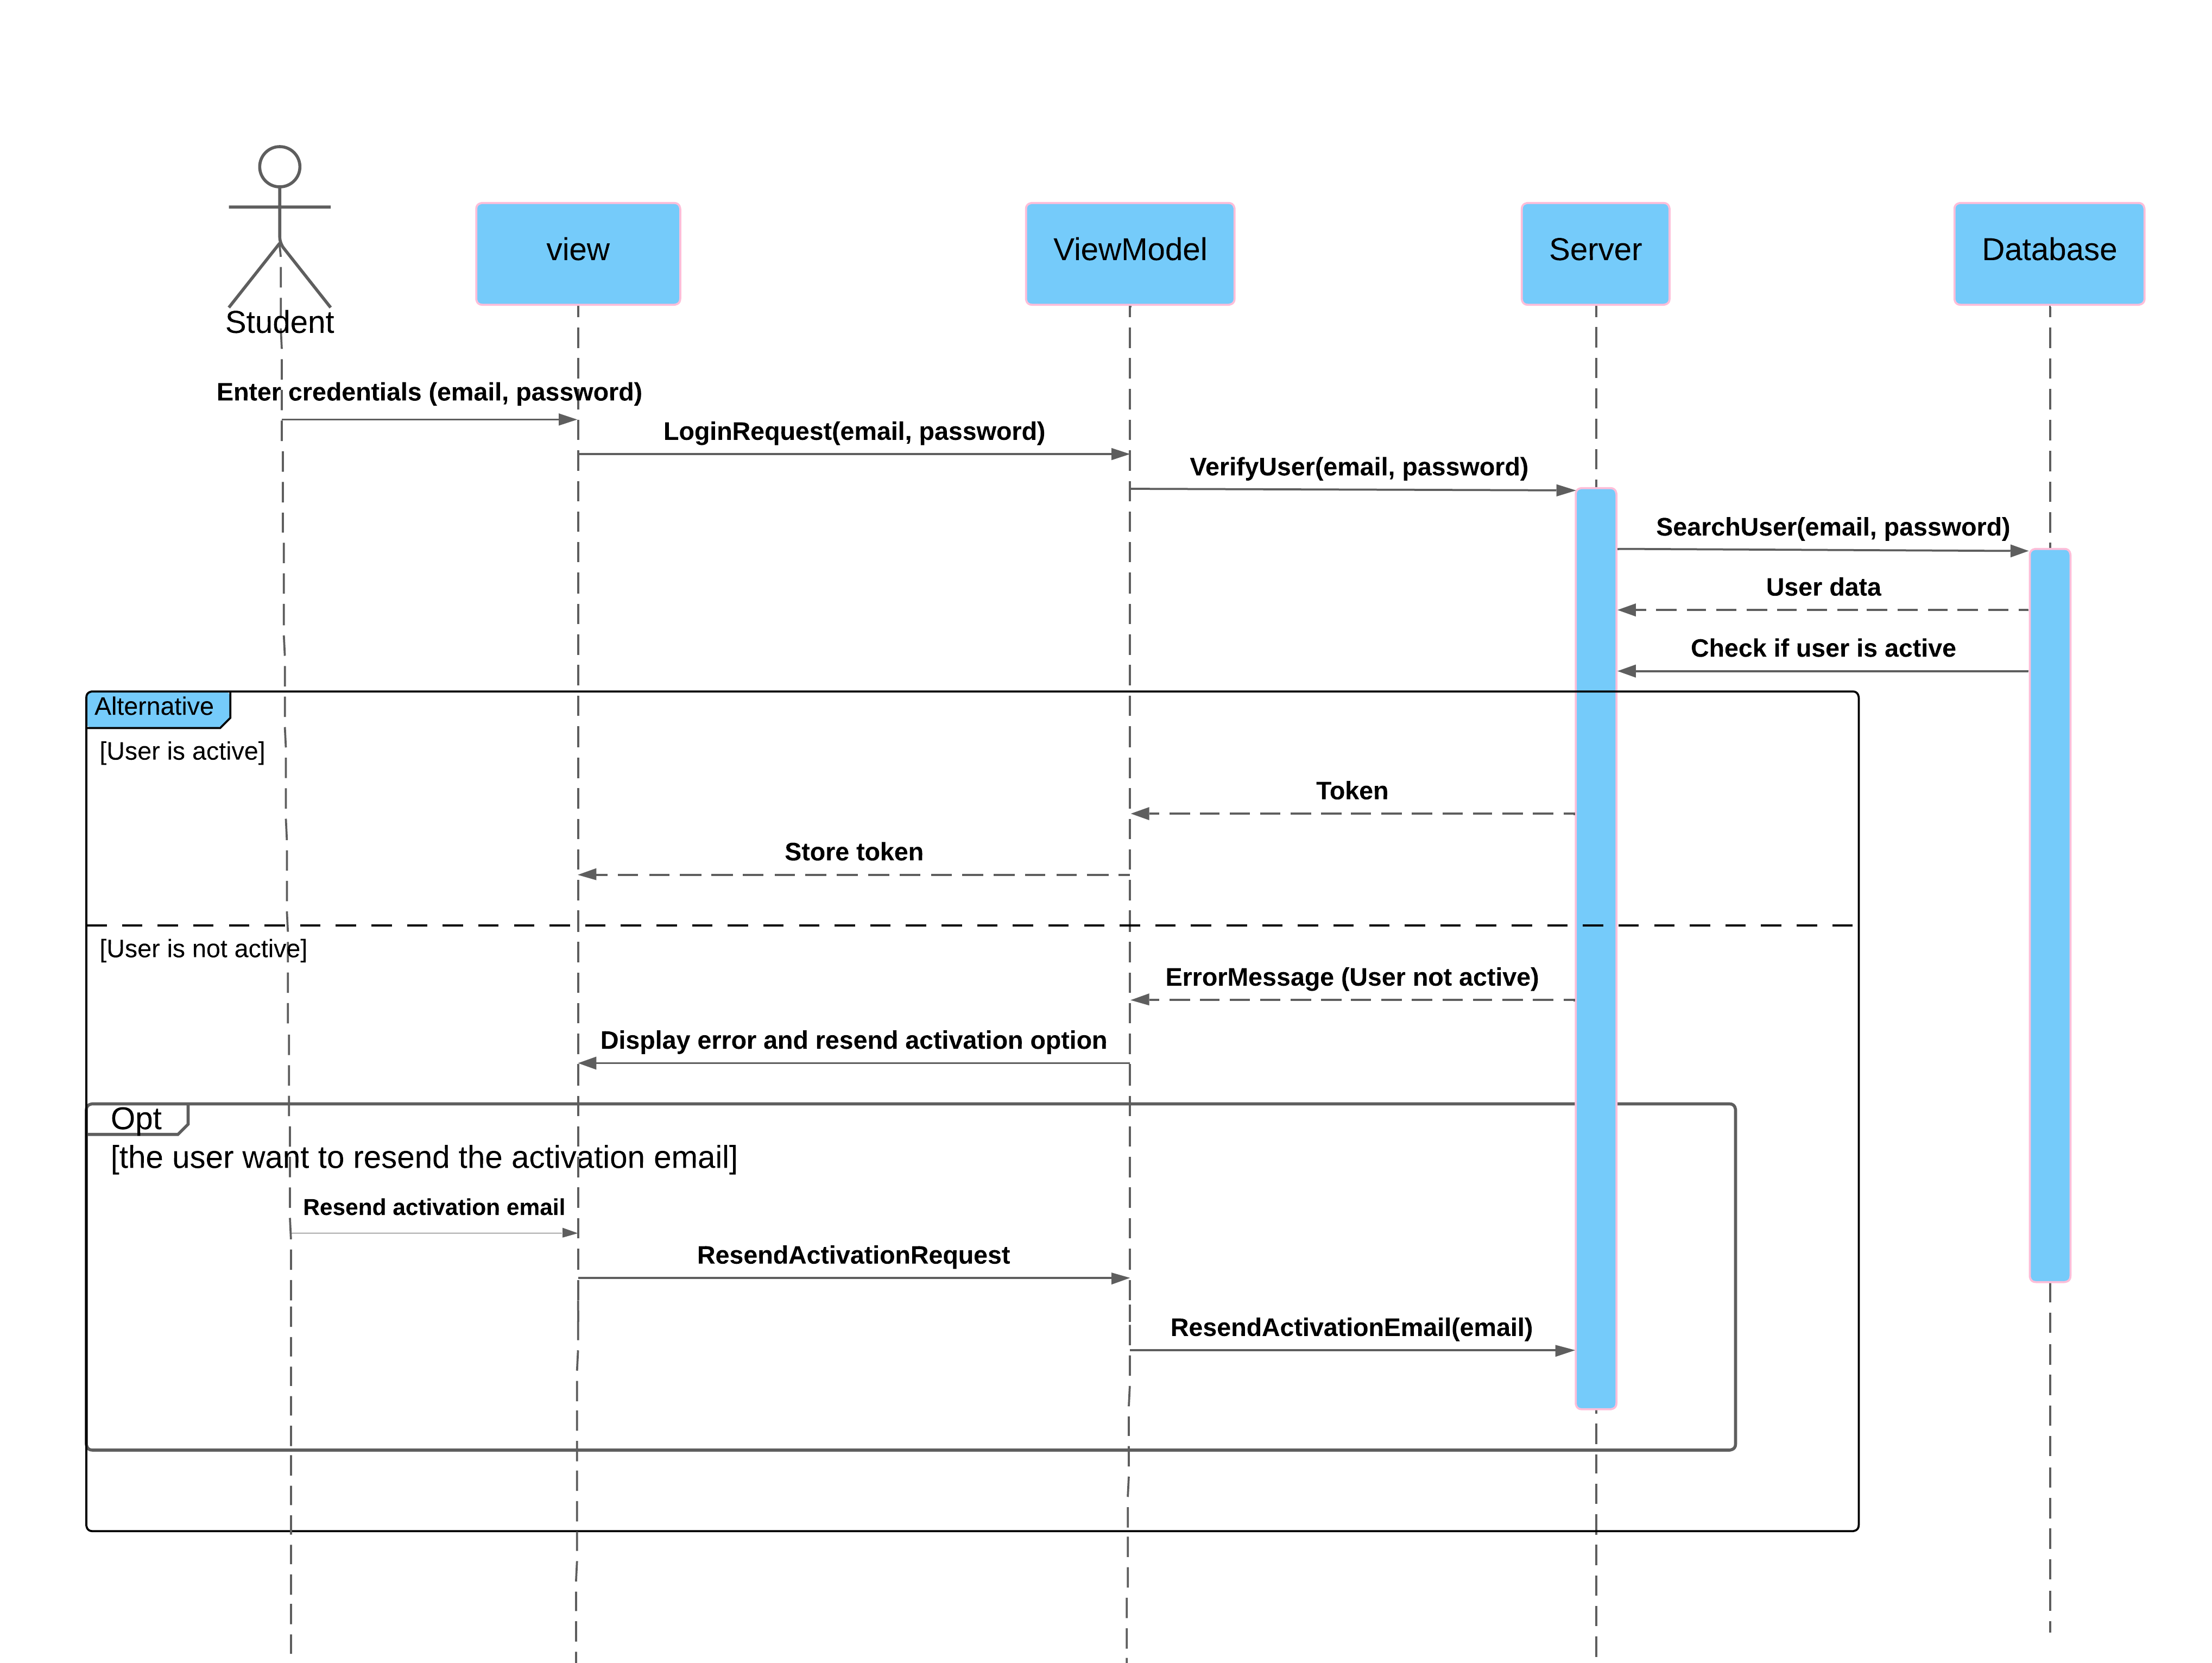
\includegraphics[scale=0.4]{diagrams/object seq diagram login.png}
            \caption{Login object sequence diagram} 
            \label{fig: Login object sequence diagram}
\end{figure}

The Signup system sequence diagram can be observed in Figure 3.4 below:

\begin{figure}[H] 
            \centering
            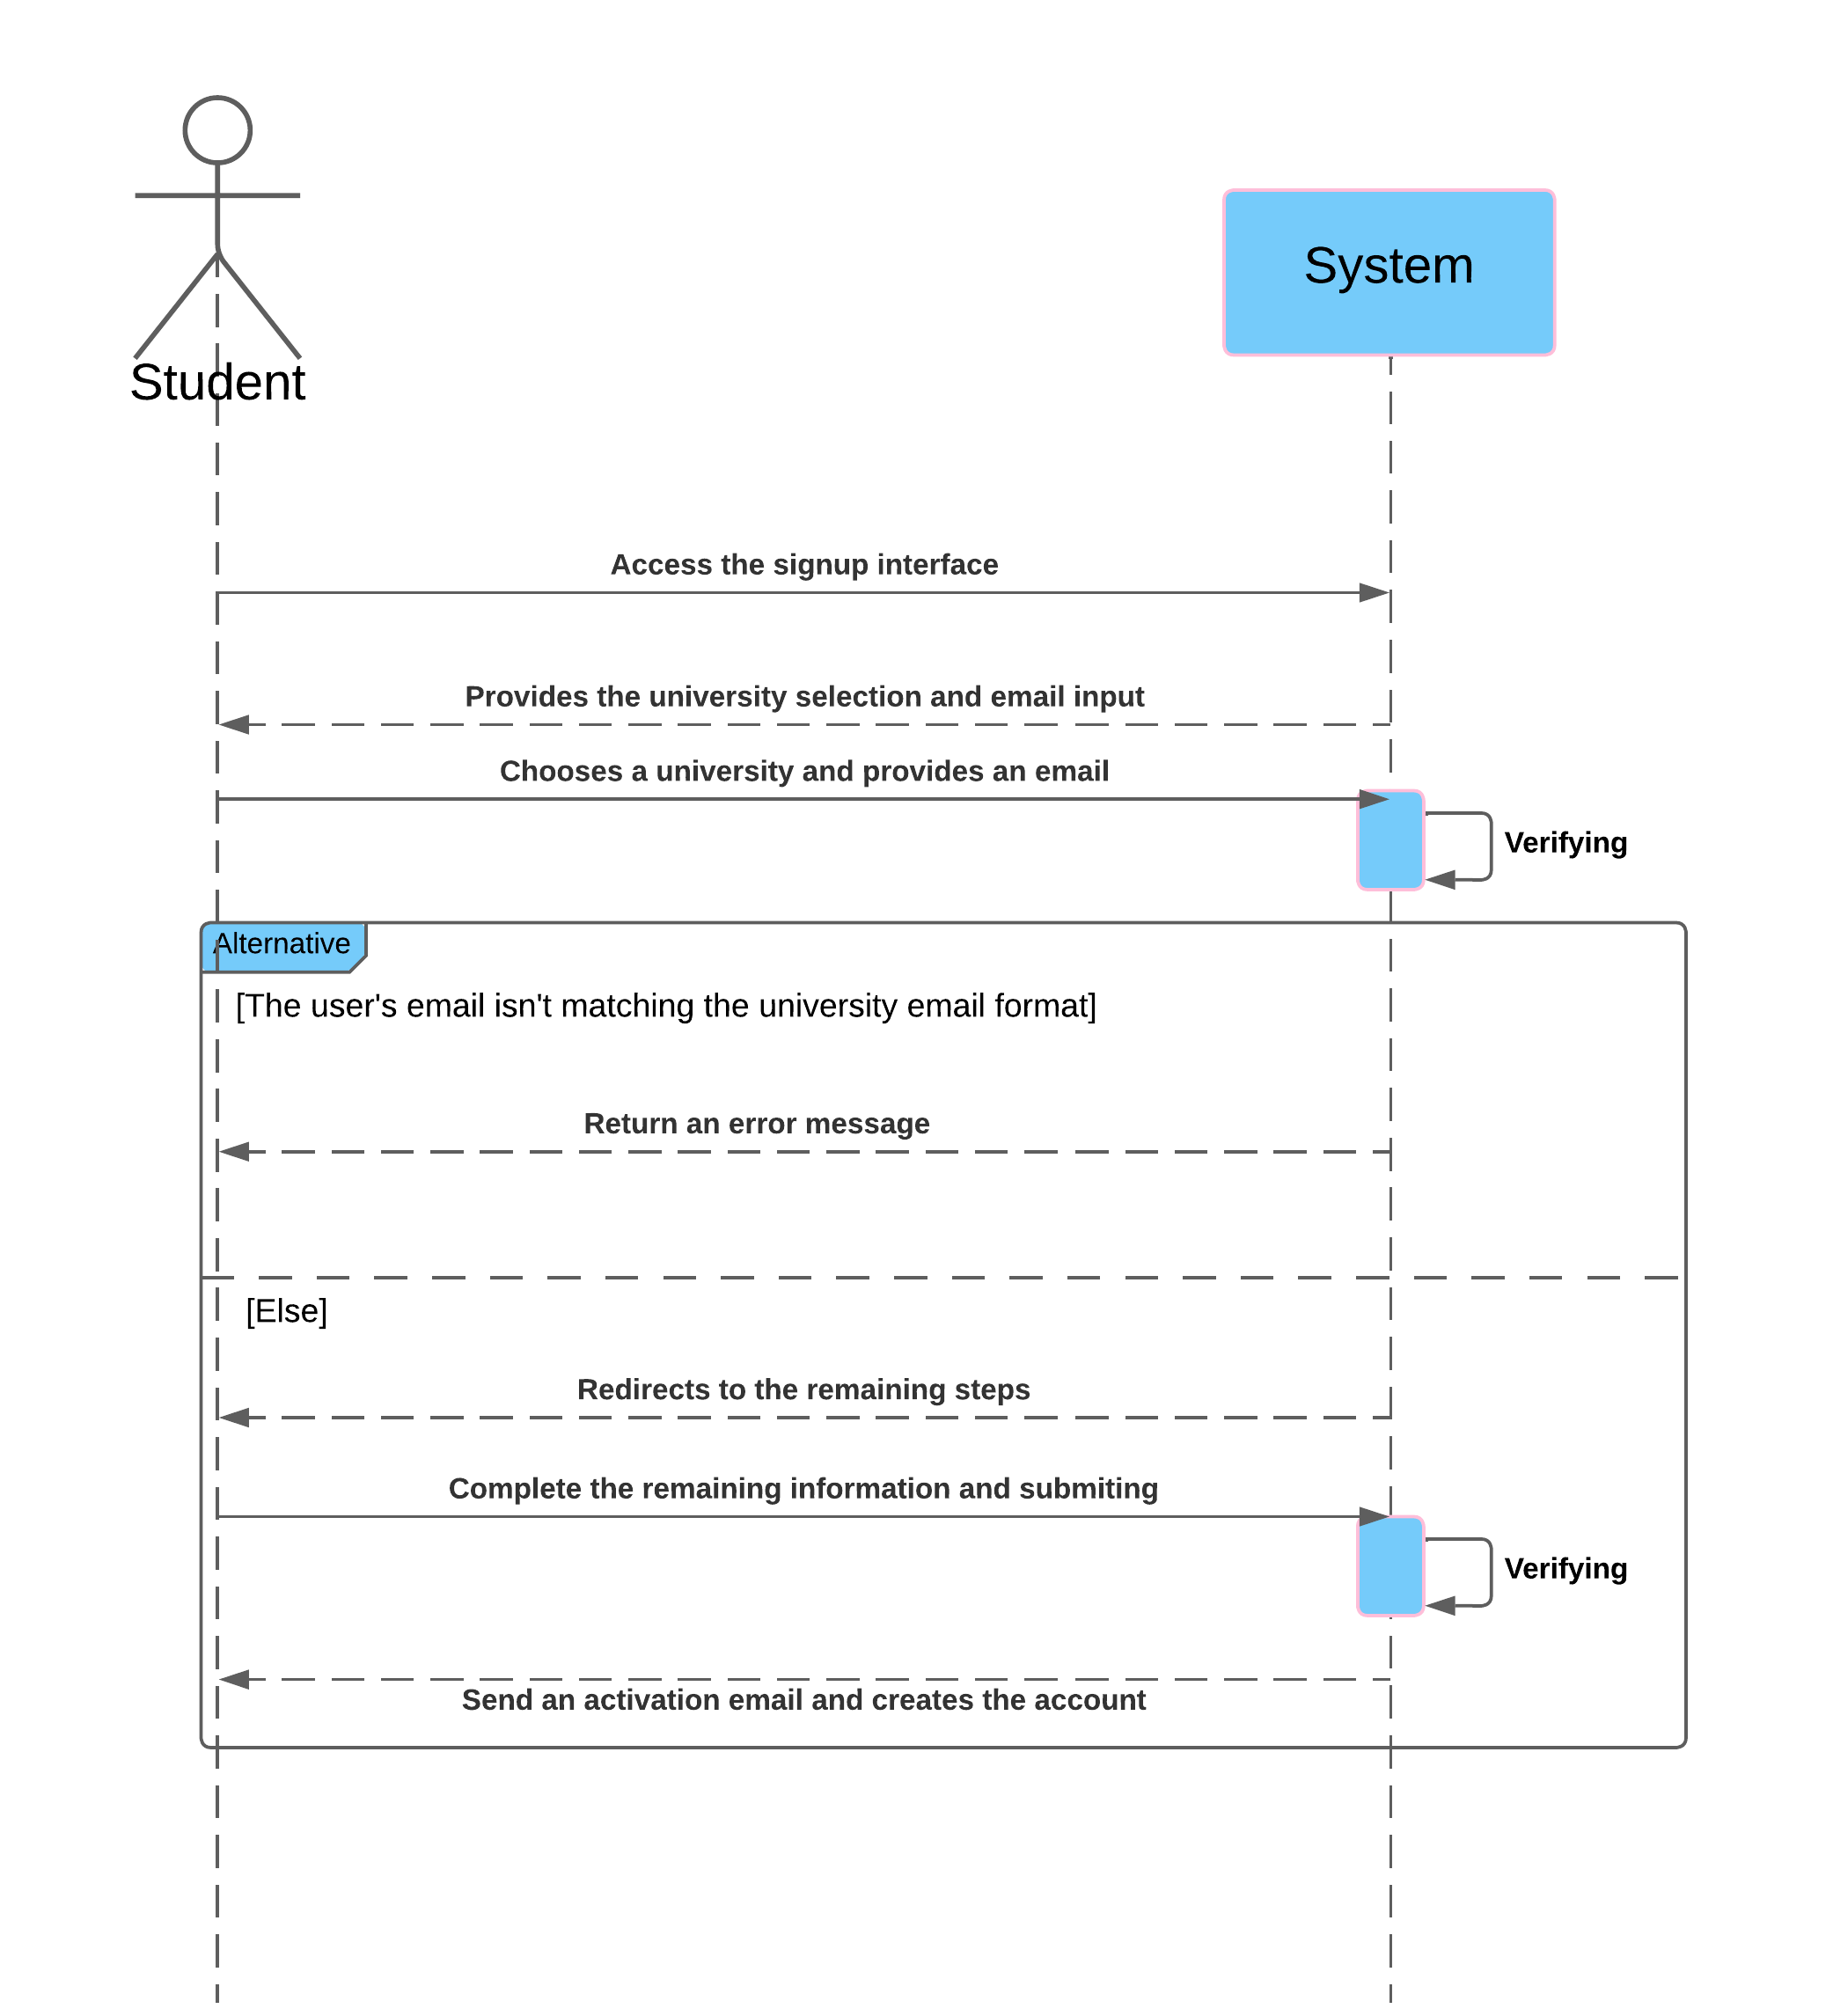
\includegraphics[scale=0.5]{diagrams/system seq diagram signup.png}
            \caption{Signup system sequence diagram} 
            \label{fig: Signup system sequence diagram}
\end{figure}

\section{Realization}
In this section, we describe what has been implemented and how the various components and functionalities identified in this Sprint have been instantiated.

\subsection{User sign-in and registration}
After taking users' needs into account, we created an easy and secure registration method. since the application is for use only by students, how did we manage to give access to the application only to students?
The company's strategy is to open access to the application every university at a time. This enables the company to collect information about the university that will be useful for the verification process. One of many verification processes is to compare the e-mail address provided by the user with the e-mail address format of the selected university using RegEx and check whether or not they match.
Once verified, the student will complete their other data and put on their face to give students an authentic experience and avoid scams and fake profiles thanks to face detection. \\

Below, we take a look at the different stages of the registration process. \\
\begin{figure}[H] 
            \centering
            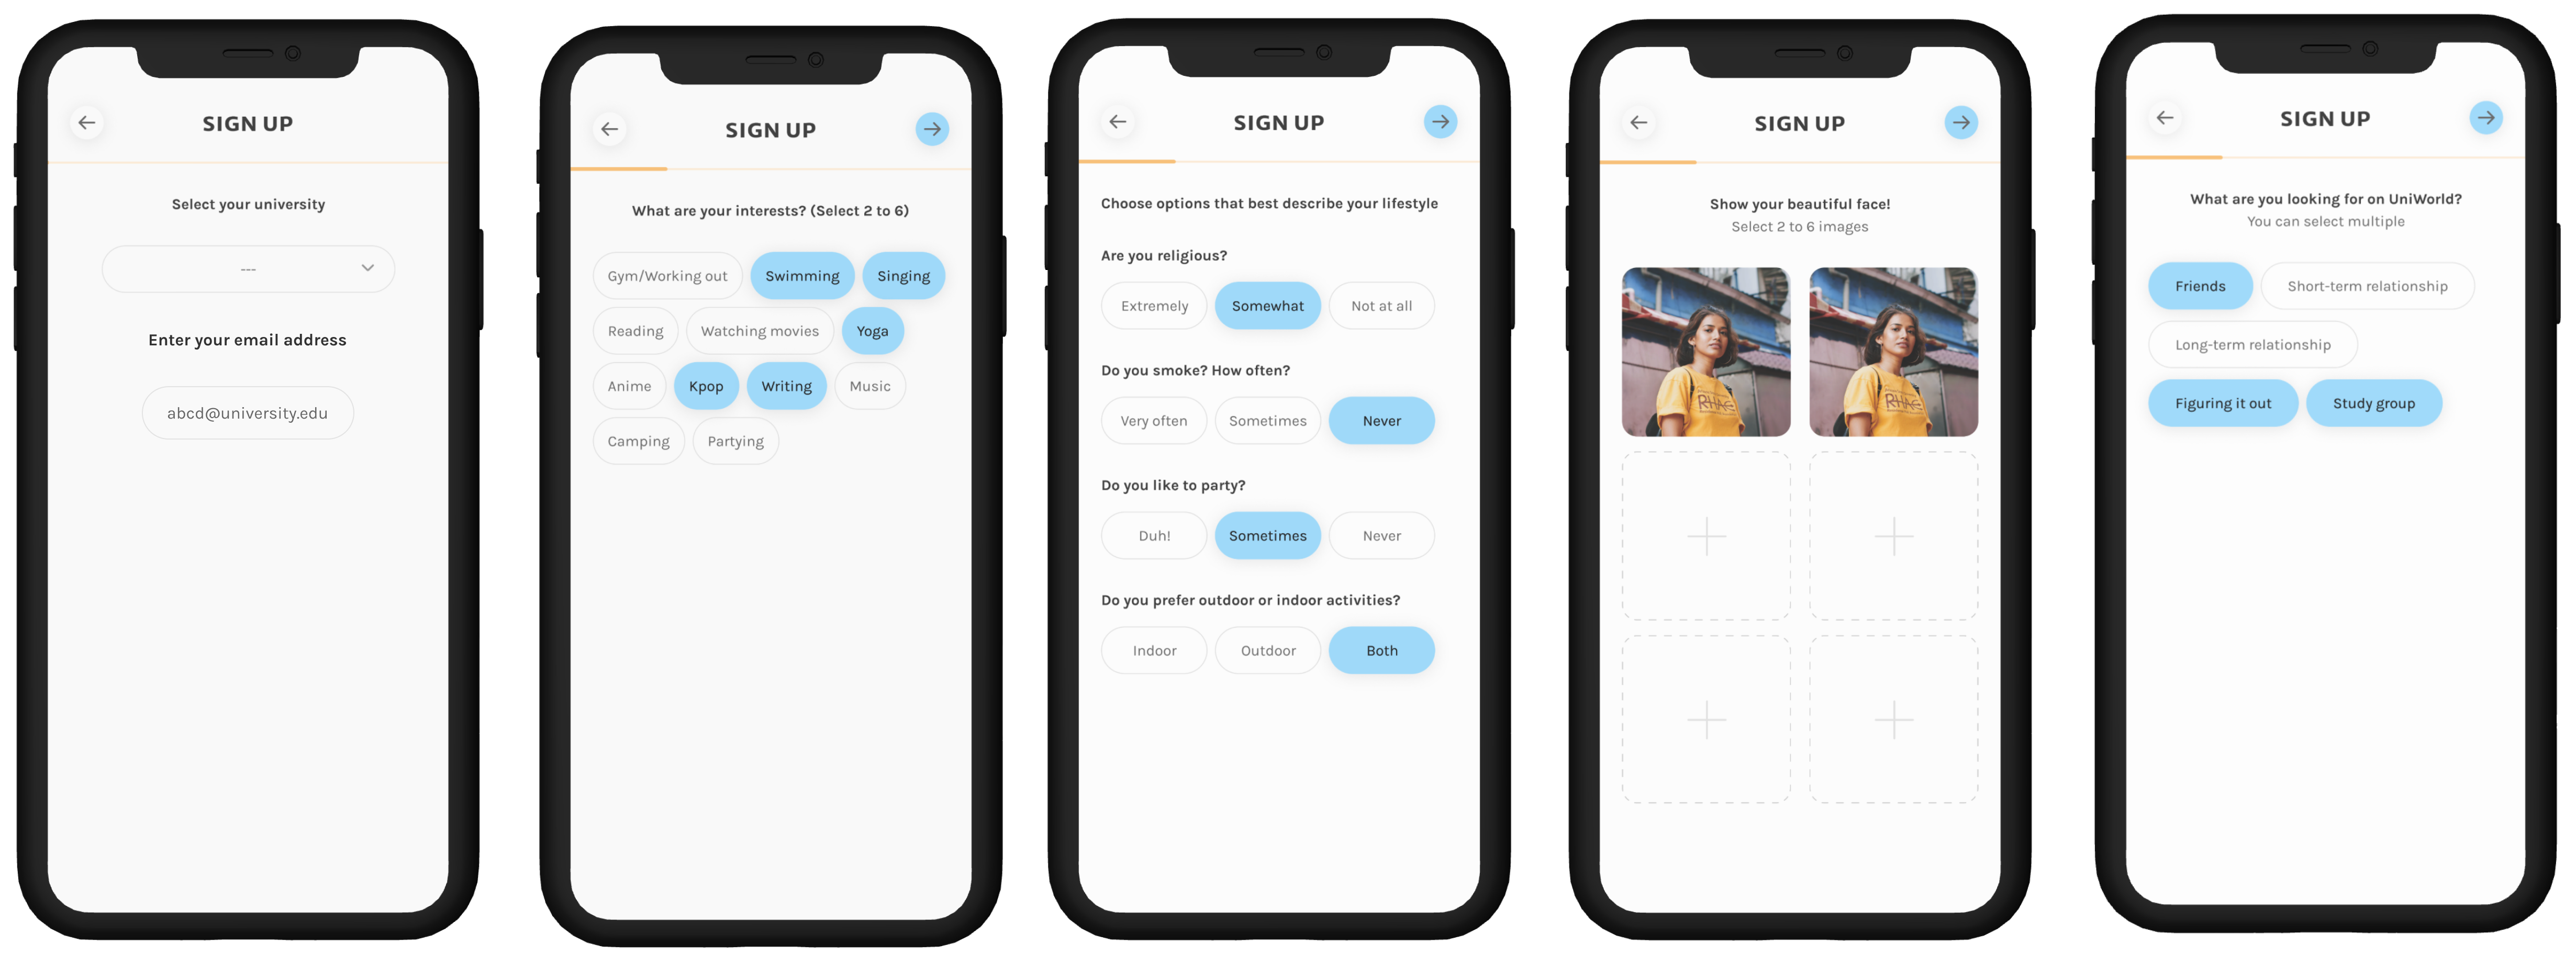
\includegraphics[scale=0.15]{steps signup.png}
            \caption{Some signup steps UI} 
            \label{fig: Some signup steps UI}
\end{figure}
Creating a new account involves hashing the password given by the user, After that it sends a verification mail to the user to activate the account in order to prevent the creation of emails with fake or non-existent emails After the creation of a new account, the login process is relatively simple but optimized for security, the use of JWT for session control has brought unbelievable results in the control of authentication. After activation of the account,  the user inputs his credentials then the system checks whether the user exists and whether his/ her credentials are correct. Once this has been verified, the backend issues out a token to the application and saves it before it is used as a means to authenticate the application’s services. 
The following figure shows the login UI
\begin{figure}[H] 
            \centering
            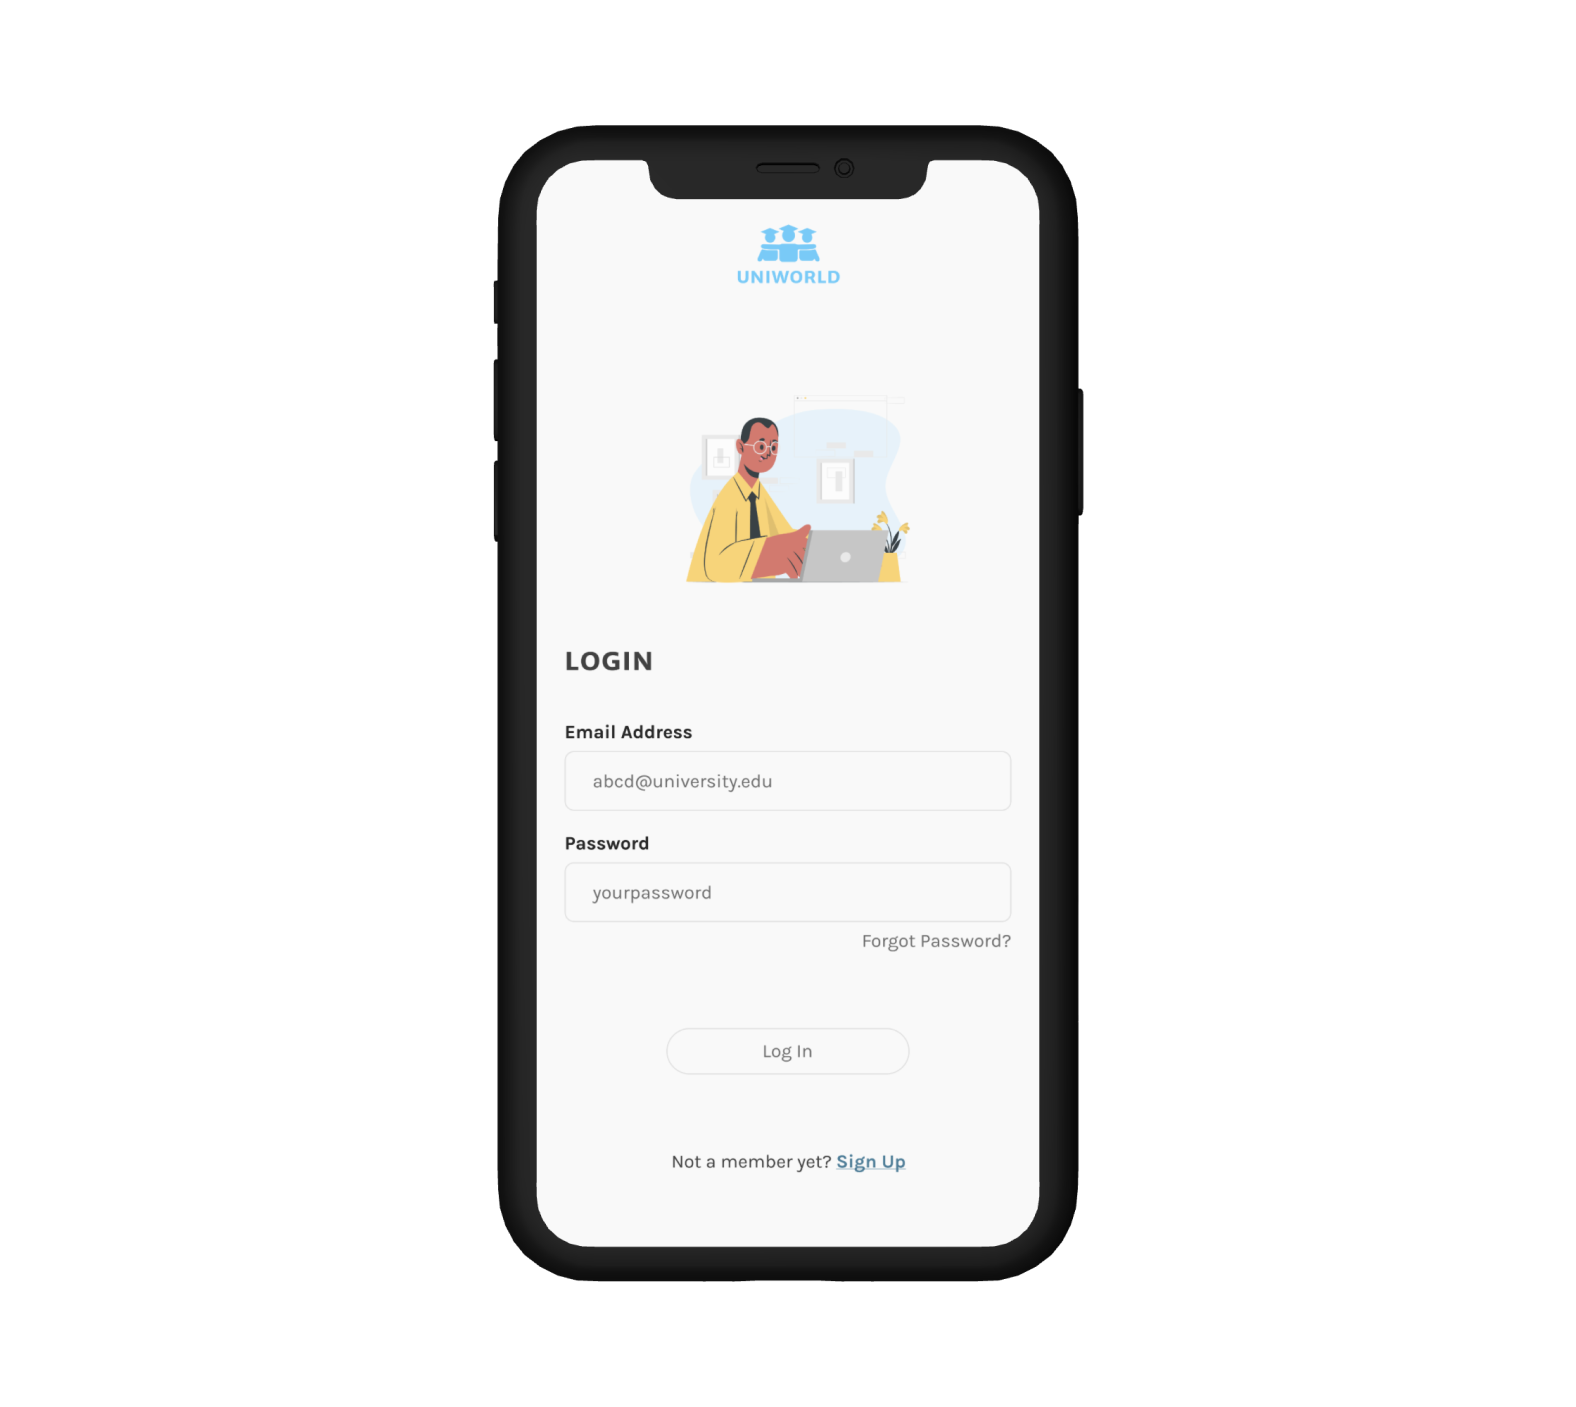
\includegraphics[scale=0.2]{login UI.png}
            \caption{Login UI} 
            \label{fig: Login UI}
\end{figure}
\begin{figure}[H] 
            \centering
            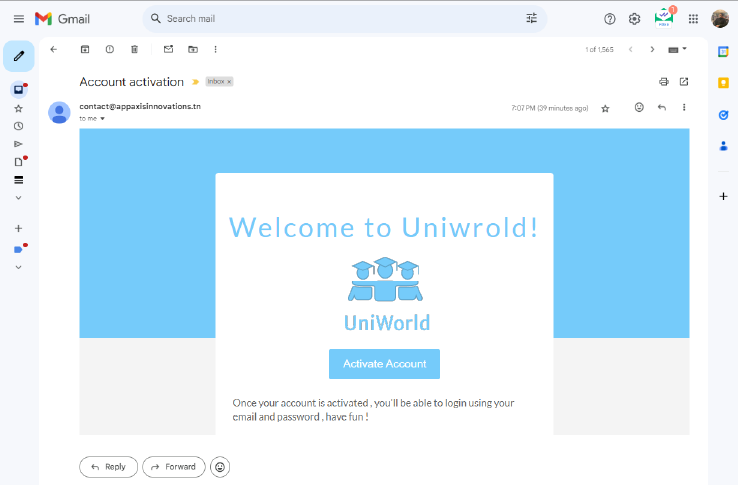
\includegraphics[scale=0.5]{account actiavation mail.png}
            \caption{account activation email} 
            \label{fig: account activation email}
\end{figure}
\subsection{Account management}
After creating an account and logging in, users can manage their account and modify some of the information they have already provided. But first, the system needs the user's token so that he can modify his information.
The account management interface is shown below. 
\begin{figure}[H] 
            \centering
            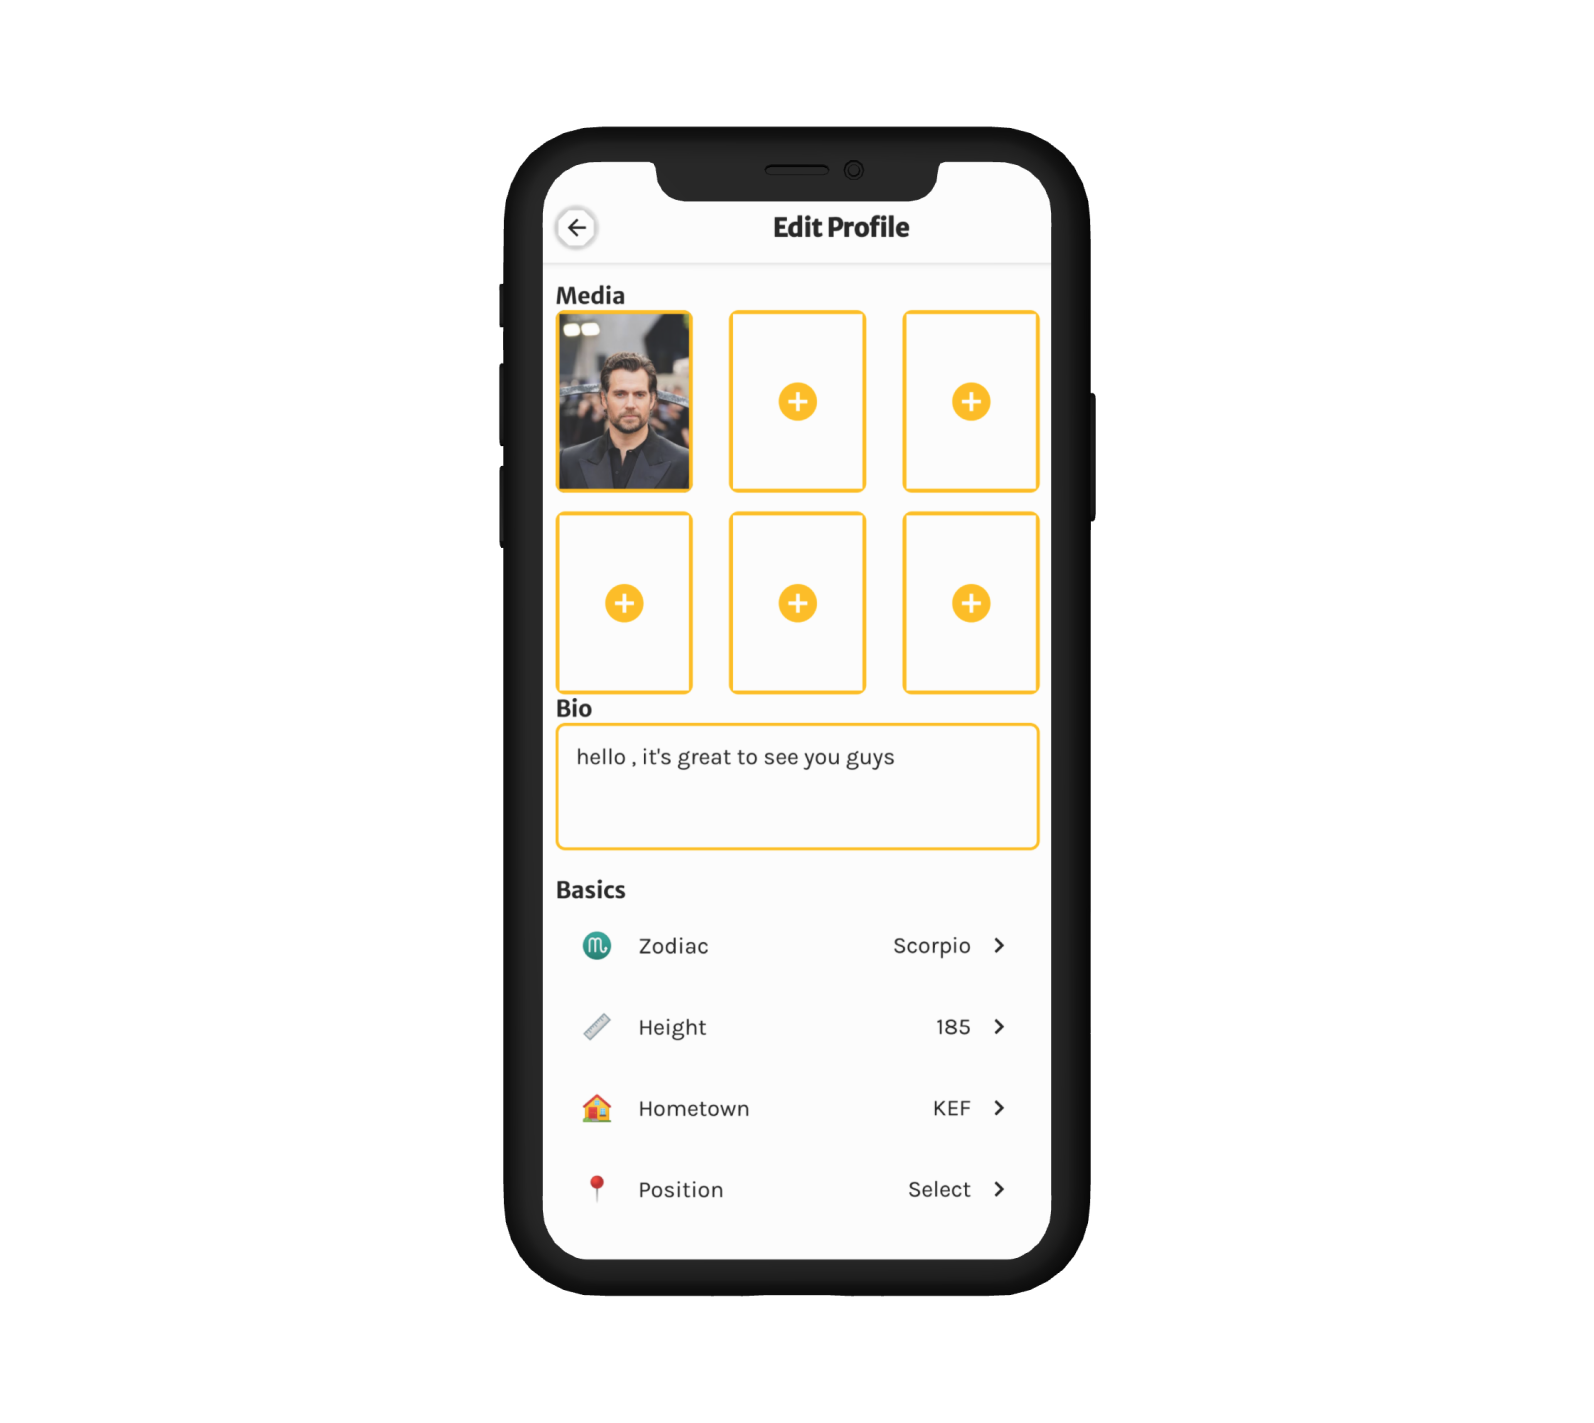
\includegraphics[scale=0.2]{profile managment UI.png}
            \caption{profile management UI} 
            \label{fig: profile management UI}
\end{figure}
\subsection{Password restoration}
Suppose the user has forgotten his password, this will be an inconvenience as he will no longer be able to log in, so we provide a password restoration process so that the user can recover his password safely, first, he types his email, then he checks his mailbox to find a 4-digit code that he can put into the application to finally change his password.
The figure below shows the steps involved in restoring a password.
\begin{figure}[H] 
            \centering
            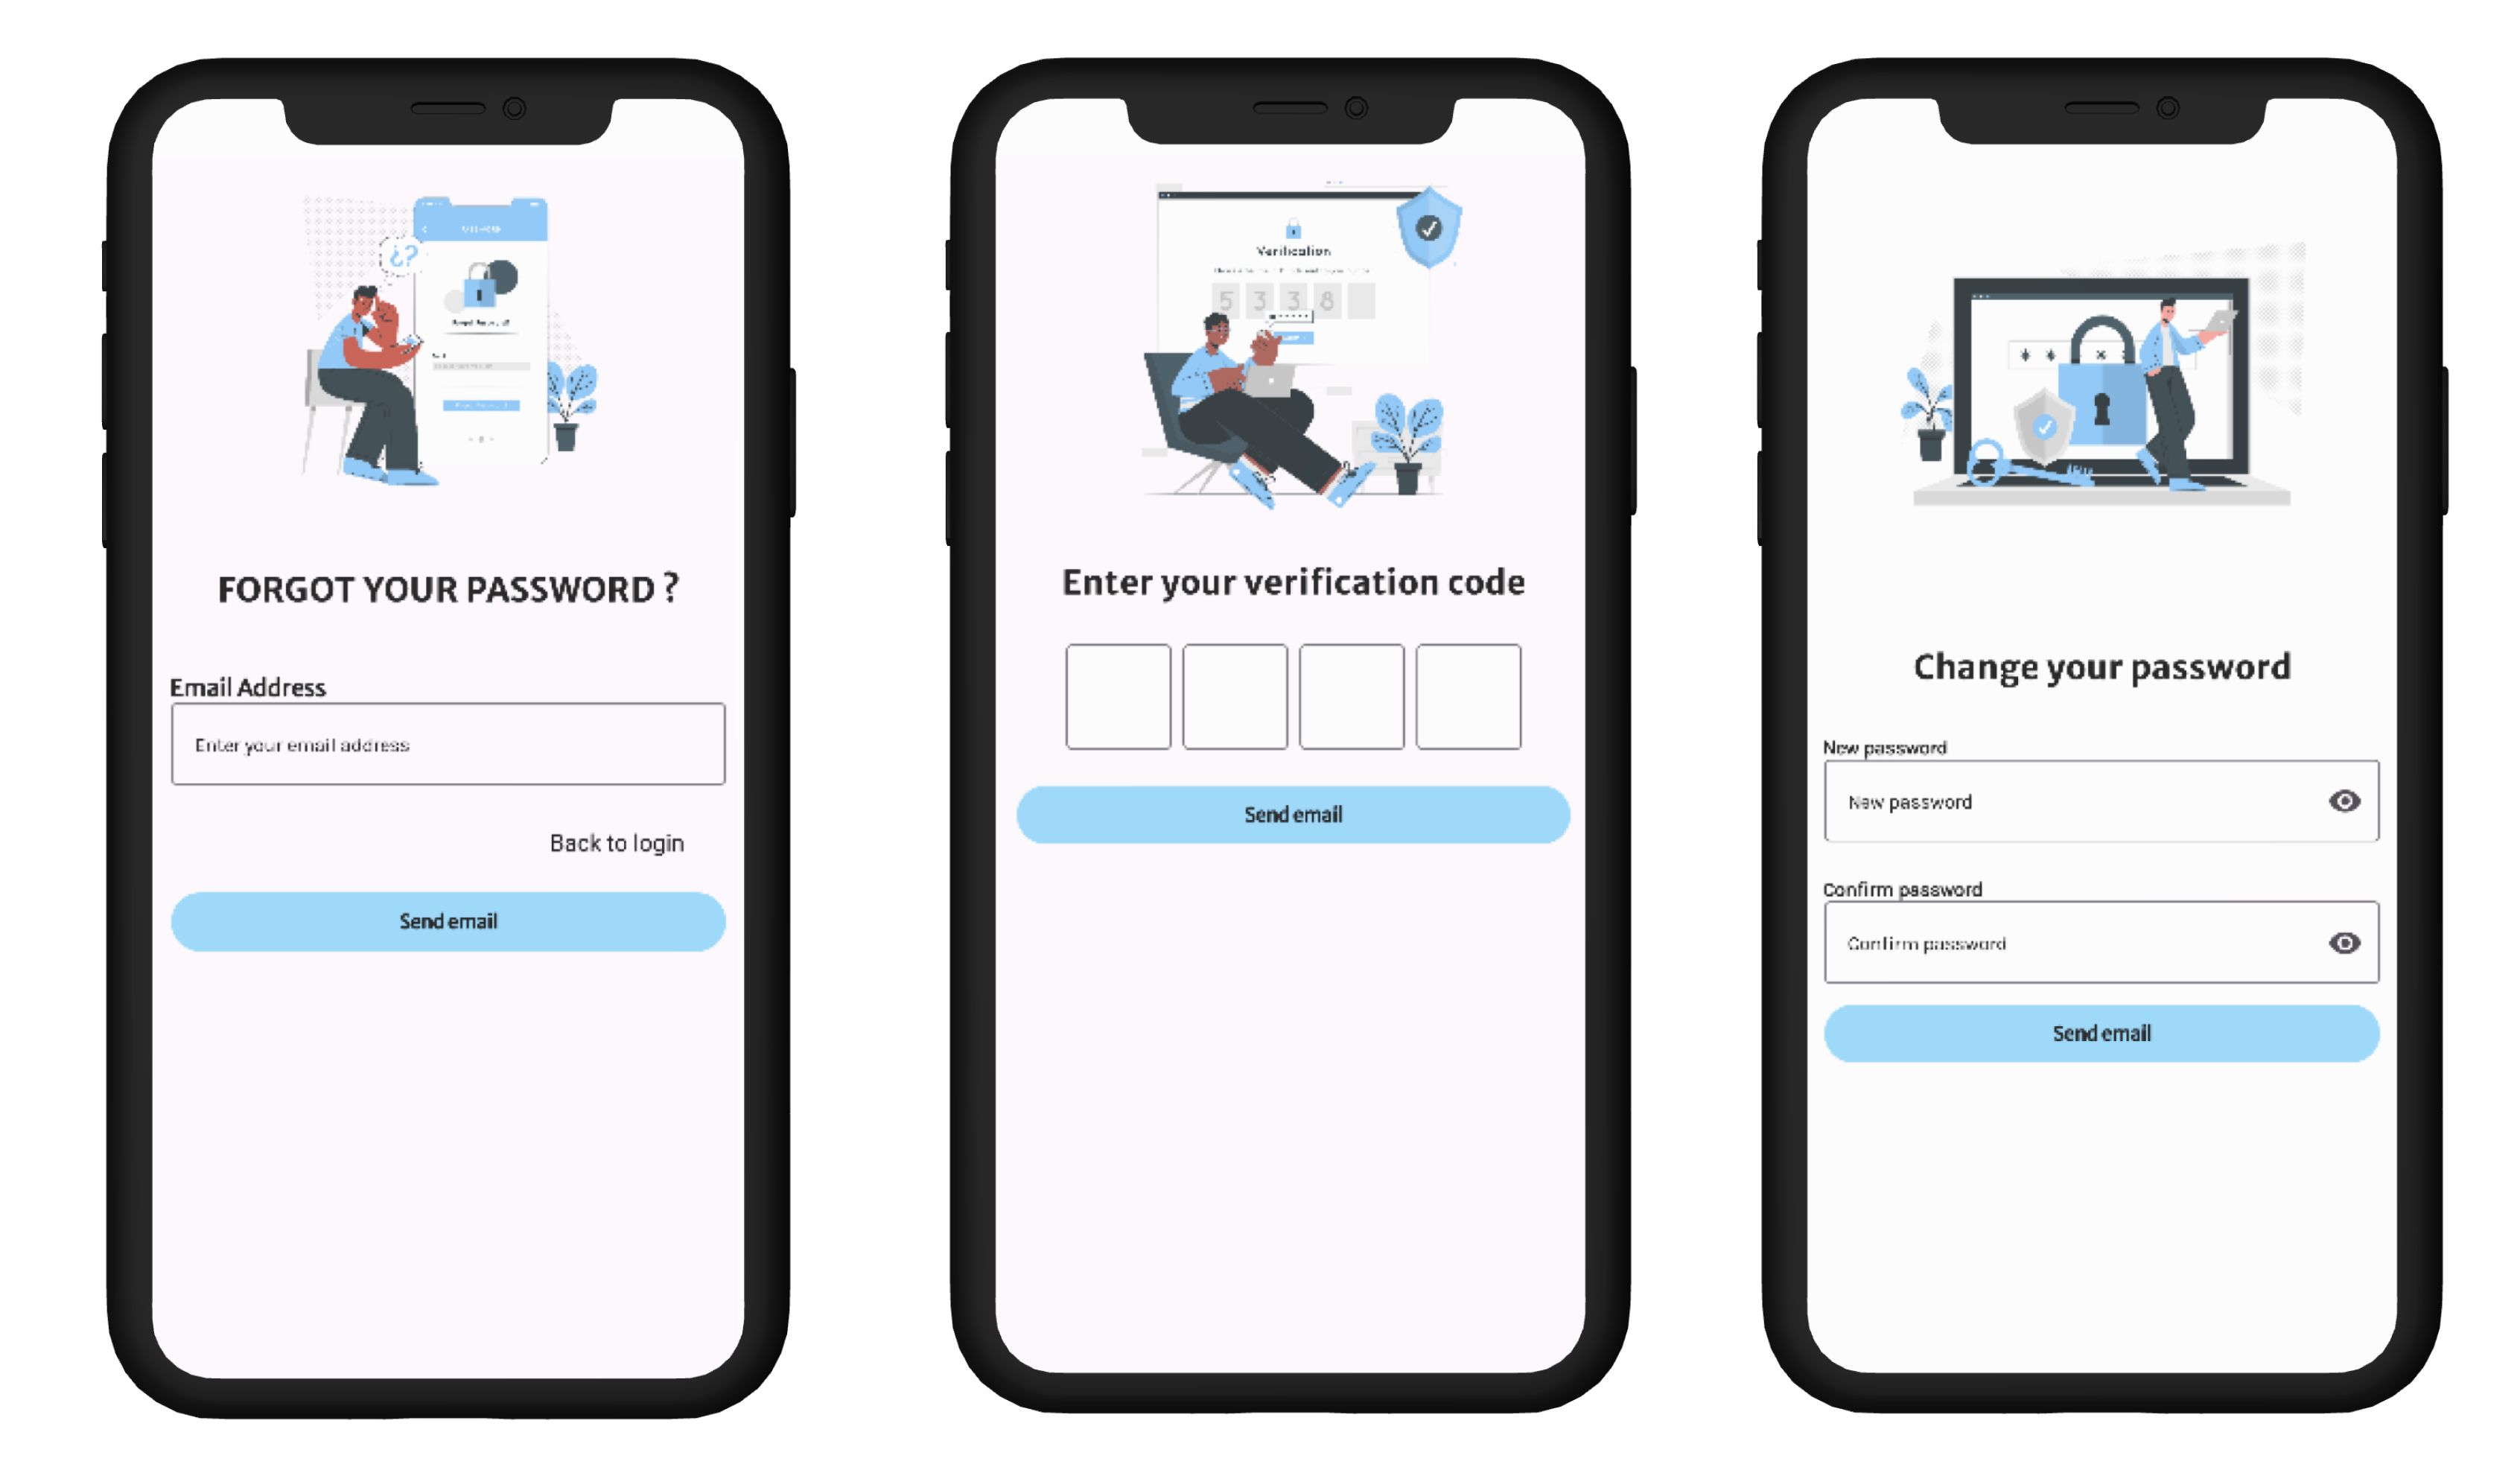
\includegraphics[scale=0.2]{forget password signup.png}
            \caption{forget password UI} 
            \label{fig: forget password UI}
\end{figure}
\section*{Conclusion}
\addcontentsline{toc}{section}{Conclusion}
Sticking to the tradition of the chosen methodology, the first sprint introduced a design of the features that are complete for managing users and their authentication. The fact that it is possible to test and specifically these features in the subsequent sprints is the point that brings the team closer to the goal and the great immersive experience. 


\chapter{Sprint 2: Uni-match}



\section*{Introduction}

\addcontentsline{toc}{section}{Introduction}

In this chapter, we'll be exploring the second Sprint, which focuses on the design and implementation of uni-world's social features.

\section{Sprint Backlog}
To start, we outline the work to be done in this sprint. The schedule for this iteration
involves the user stories described in the following Table 3.1:

\begin{longtable}{|l|p{6cm}|p{8cm}|}
\hline
Sprint & User story & Task\\
\hline
\endfirsthead

\multicolumn{3}{c}{{\bfseries}} \\
\hline
Sprint & User story & Task\\
\hline
\endhead

\hline \multicolumn{3}{|r|}{{Continued on next page}} \\ \hline
\endfoot

\hline
\endlastfoot
3 & As a student, I want to show my interest by swiping right on someone
so that I can contact them if they like me back & \begin{itemize}
    \item Create the like and match models
    \item Create the algorithm responsible for showing the users
    \item Create the matching system
    \item Create the matching feed UI
    \item Integration and testing
\end{itemize} \\ \hline

4 & As a student, I want to ignore someone I don’t find interesting & \begin{itemize}
    \item Create ignoring feature
    \item enhancing the algorithm
    \item Integration and testing
\end{itemize} \\ \hline

7 & As a student, I want to send and receive messages from my matches & \begin{itemize}
    \item Create a web socket to handle real-time communication
    \item Create the message and conversation models
    \item Create messaging feature
    \item Create messaging UI
    \item Integration and testing
\end{itemize} \\ \hline

8 & As a student, I want to see who likes me so I can decide whether or
not to like them back & \begin{itemize}
    \item Create the likes UI
    \item Integration and testing
\end{itemize} \\ \hline

9 & As a student, I want to filter my feed according to many criteria & \begin{itemize}
    \item Create user preferences schema
    \item Create filtering feature 
    \item Create filtering UI 
    \item Integration and testing
\end{itemize} \\ \hline

10 & As a student, I want to choose the gender I want to interact with & \begin{itemize}
    \item Update filtering UI 
    \item Integration and testing
\end{itemize} \\ \hline
\caption{Sprint 2 backlog}
\label{Tab: Sprint 2 backlog}
\end{longtable}


\section{ Analysis and conception}
In this section, we illustrate the sprint analysis in a more visual representation using use case diagrams and sequence diagrams of the most highlighted features:
"profiles browsing" and "Likes management".

\subsection{Use case diagrams}
\textbf{Refined use case diagram for profiles browsing: }
\begin{figure}[H] 
            \centering
            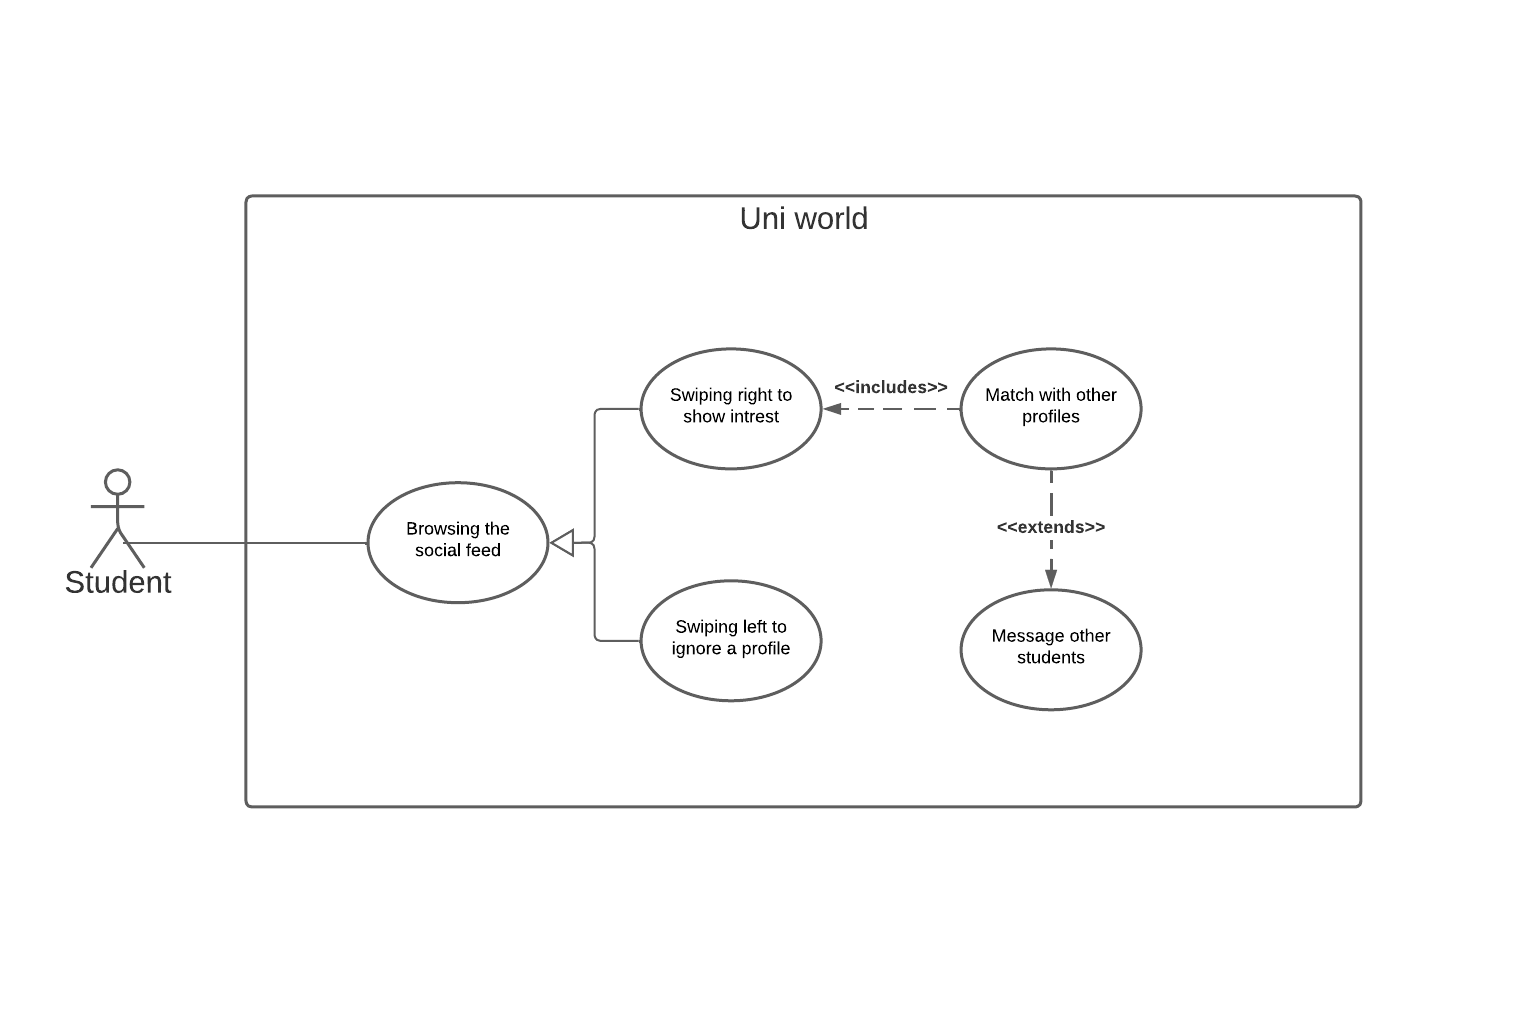
\includegraphics[scale=0.6]{diagrams/refined use case social swipe.png}
            \caption{Refined use case diagram for profiles browsing} 
            \label{fig: Refined use case diagram for profiles browsing}
\end{figure}

The diagram of the "Likes management" use case is shown in figure 3.2 :

\begin{figure}[H] 
            \centering
            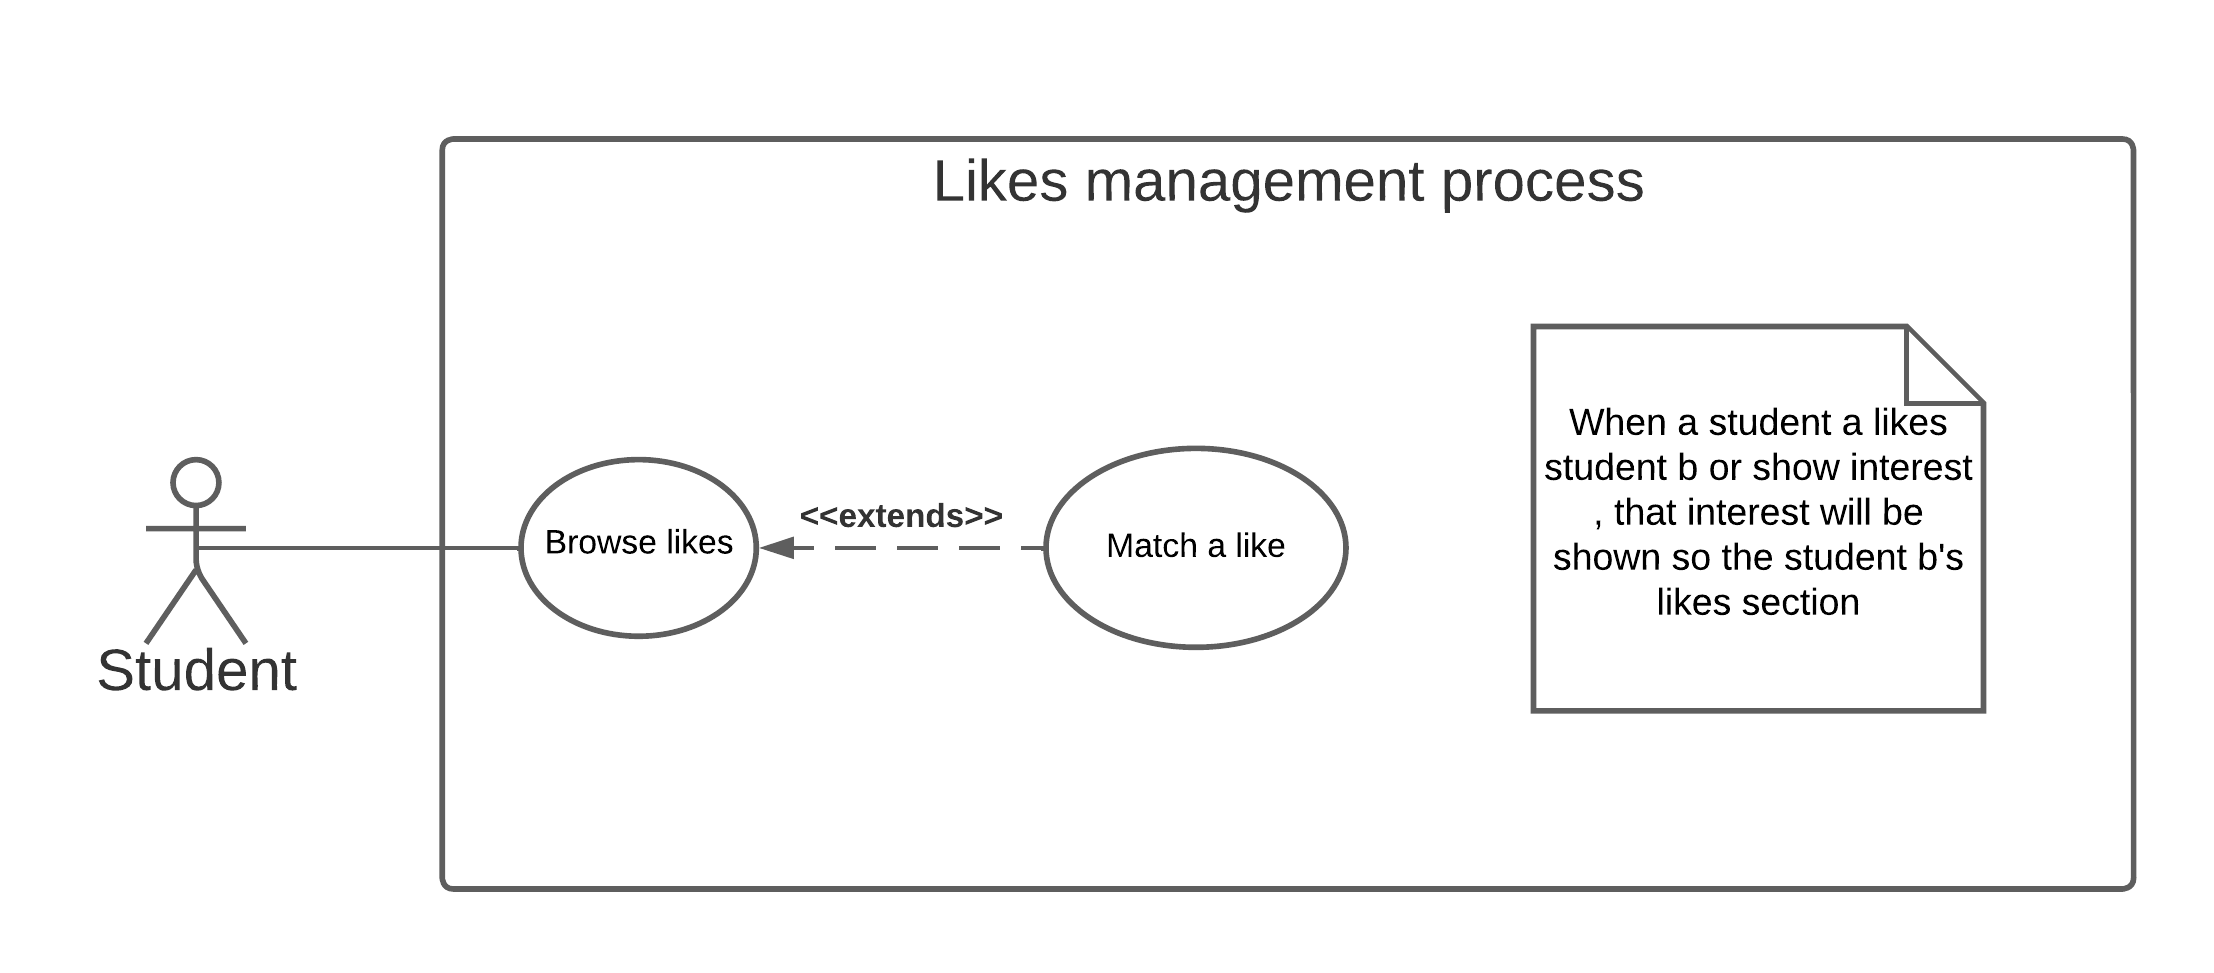
\includegraphics[scale=0.8]{diagrams/likes management use case.png}
            \caption{Likes management use case diagram} 
            \label{fig: Likes management use case diagram}
\end{figure}

\subsection{Use case textual descriptions}
Textual descriptions of the "profiles browsing" use case are illustrated in table 4.2 below:
\begin{longtable}{|c|p{10cm}|}
\hline
Use Case & Description \\\hline
Name & profiles browsing use case \\\hline
Preconditions & the student must be authenticated and have an active account \\\hline
Postconditions & After matching, the student can send a message of his/her choice to the other students who are in the system. This communication function mainly helps profiles that are matched to be able to communicate effectively. \\ \hline
Main Flow & 
\begin{enumerate}
    \item Student opens the feed screen.
    \item   Student passes through the profiles with the help of the system known as “Uni match”
    \item Such action enables them to see the profiles of other users and get two choices:
        \begin{itemize}
            \item   Swipe right: Expresses the student’s liking for a profile.
            \item   Swipe left: Fails to heed a profile.
        \end{itemize} 
        \item the action will be incorporated into the system. 
        \item The selected profiles are “matched”.
\end{enumerate}

\\\hline
Alternative Flows & 
    if there is a network error, an error message appears
\\\hline
\caption{Textual descriptions of the profiles browsing use case}
\label{Tab: Textual descriptions of the profiles browsing use case}
\end{longtable}

The use case textual description of "Likes management" is illustrated in the
following Table 3.3:

\begin{longtable}{|c|p{10cm}|}
\hline
Use Case & Description \\\hline
Name & Likes management use case \\\hline
Preconditions & user A and User B must both have an active account and must both be authenticated \\\hline
Postconditions & user A and User B can match if user A likes User B back
\\\hline
Main Flow &
Let's suppose we have two users A and B
\begin{enumerate}
    \item User A will swipe right (shows interest) to user B
    \item User B will receive a new like in his likes section 
    \item User B can
       \begin{itemize}
        \item Return the like to User A so they can match
        \item Ignore the like so it can eventually disappear once he swipes left on user A's profile in the feed
    \end{itemize} 
\end{enumerate}
\\\hline
Alternative Flows & \begin{itemize}
    \item if User B swipes left (ignores) User A profile, the like will be automatically deleted
    \item if there is a network error, an error message appears
\end{itemize}
\\\hline
Non-functional Requirements & \begin{itemize}
    \item The Like management will have a user-friendly UI
\end{itemize}
\\\hline
\caption{Textual descriptions of the Likes management use case}
\label{Tab: Textual descriptions of the Likes management use case}
\end{longtable}

\subsection{Sequences diagram}
The Profiles browsing object sequence diagram can be observed in Figure 4.3 below:

\begin{figure}[H] 
            \centering
            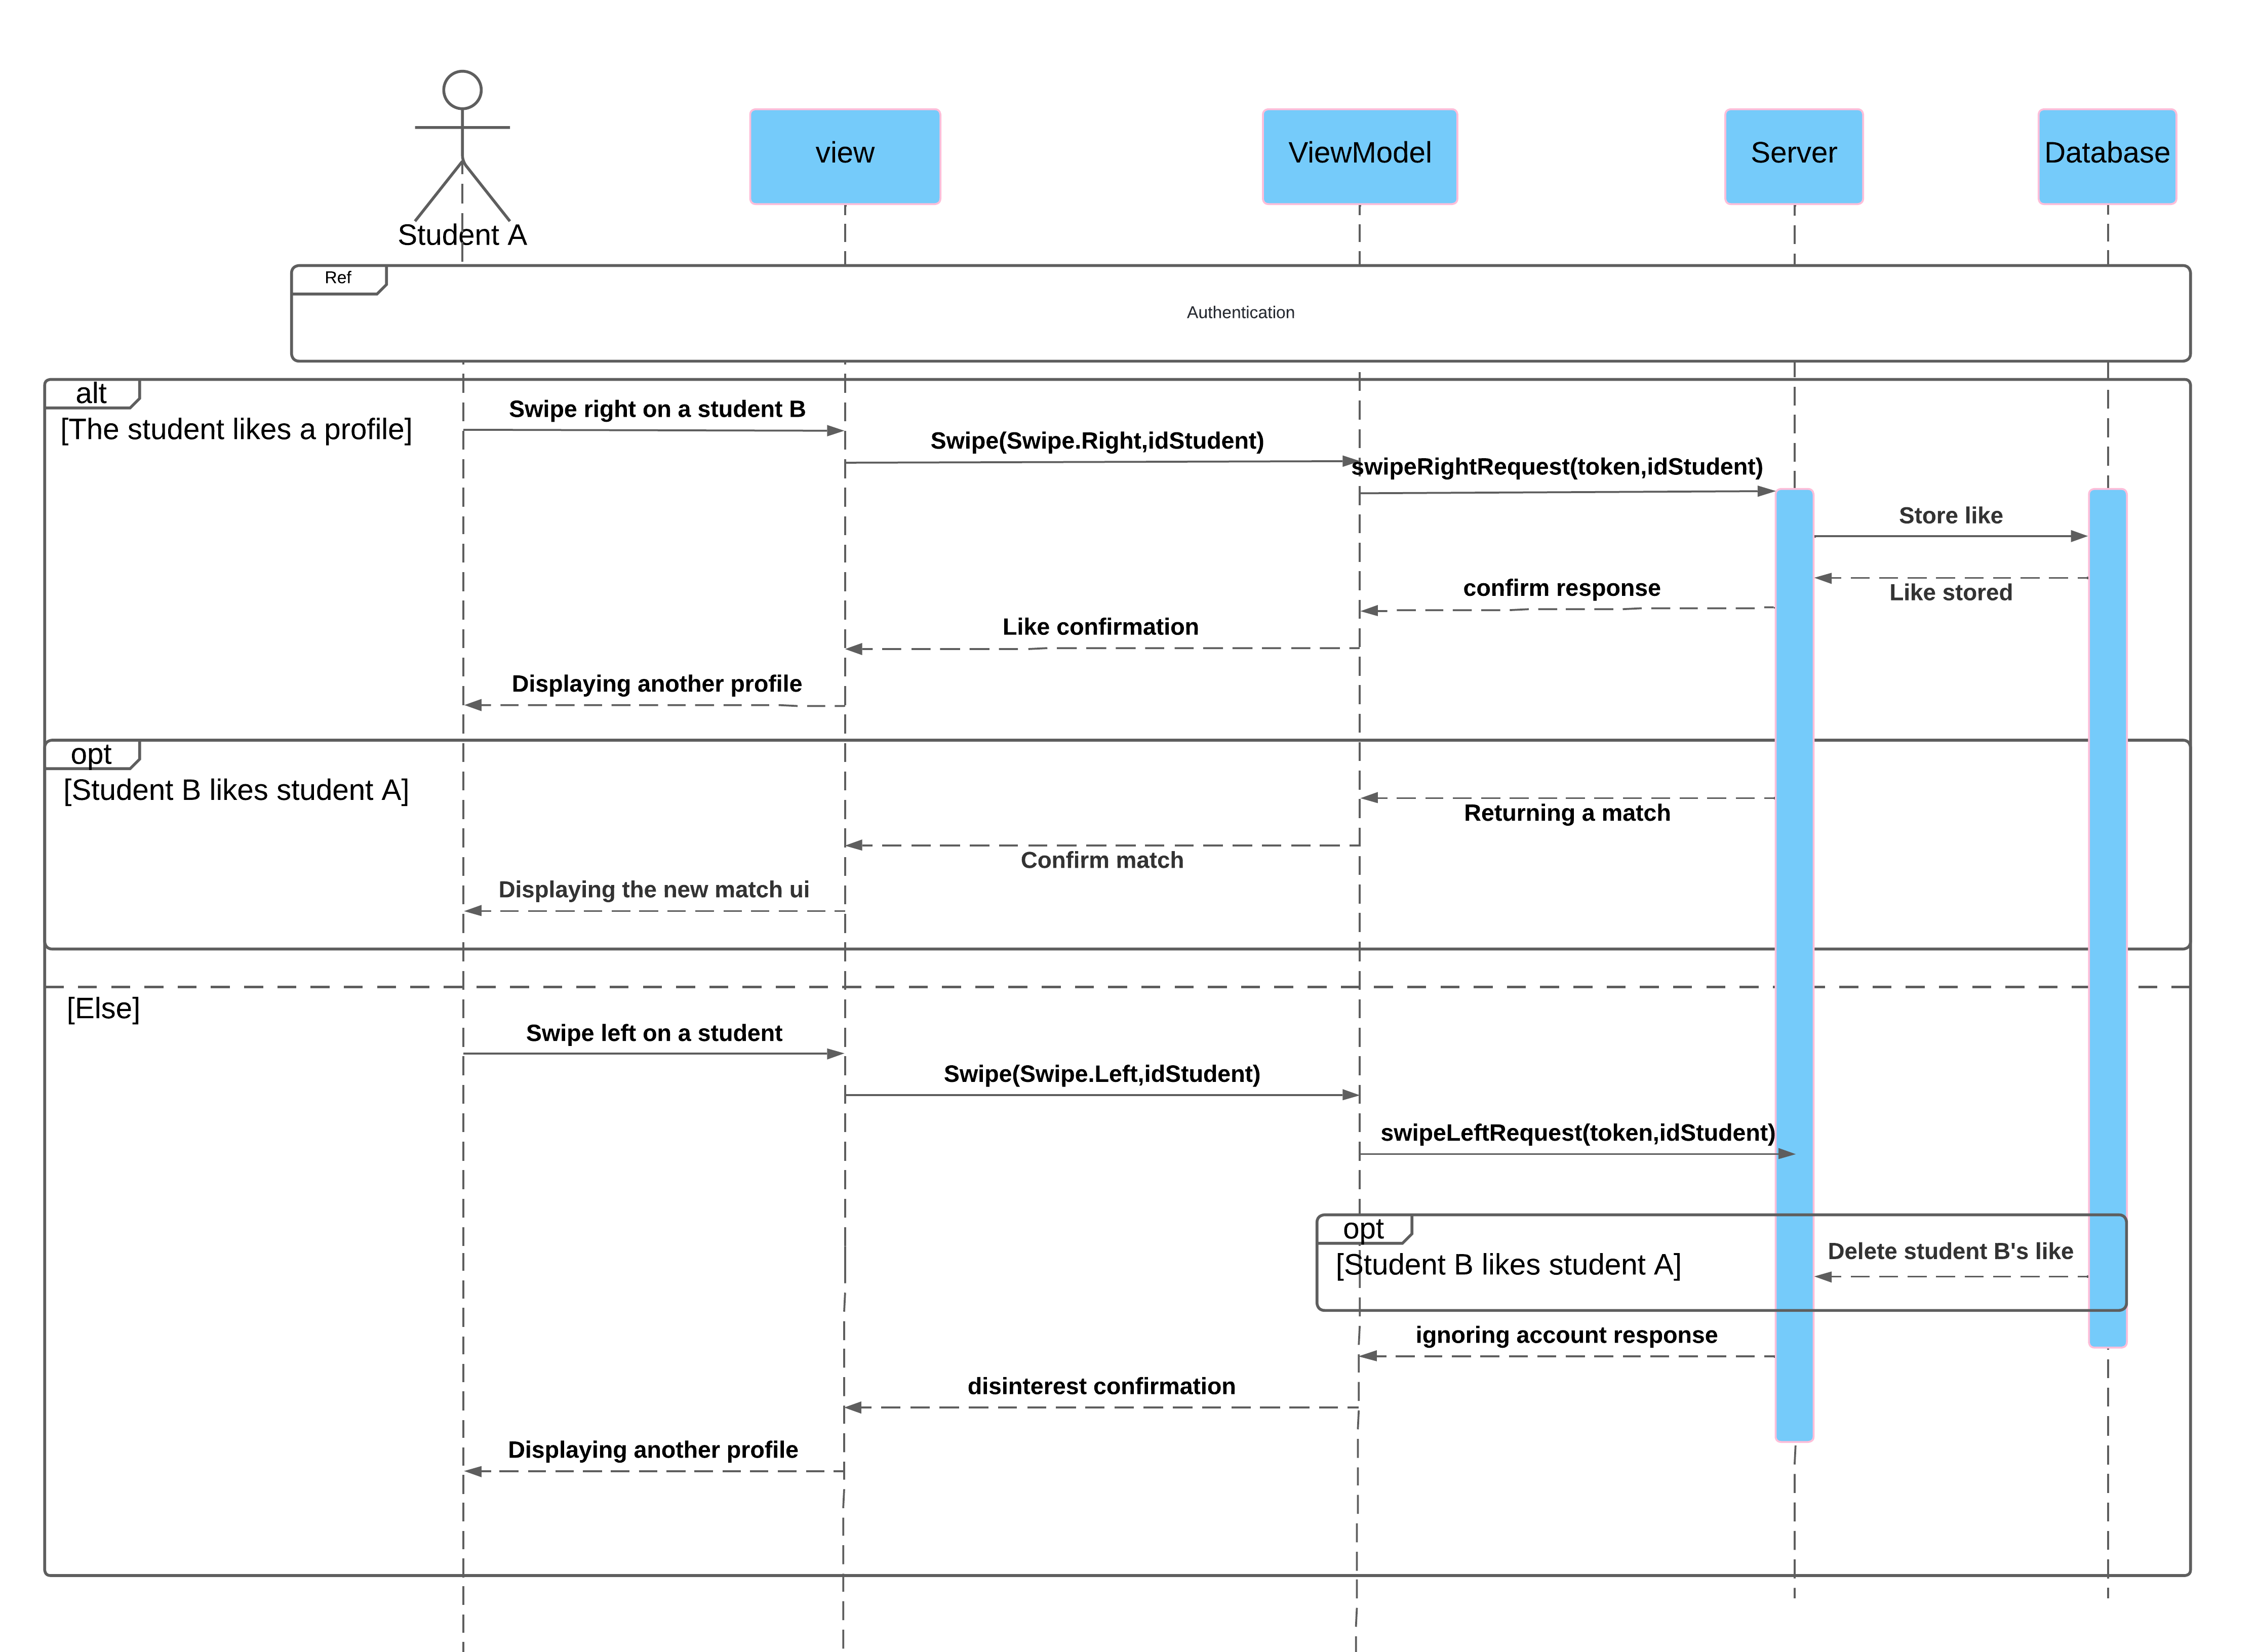
\includegraphics[scale=0.4]{diagrams/profile browsing seq diagram.png}
            \caption{Profiles browsing object sequence diagram} 
            \label{fig: Profiles browsing object sequence diagram}
\end{figure}

The Likes management system system sequence diagram can be observed in Figure 4.4 below:

\begin{figure}[H] 
            \centering
            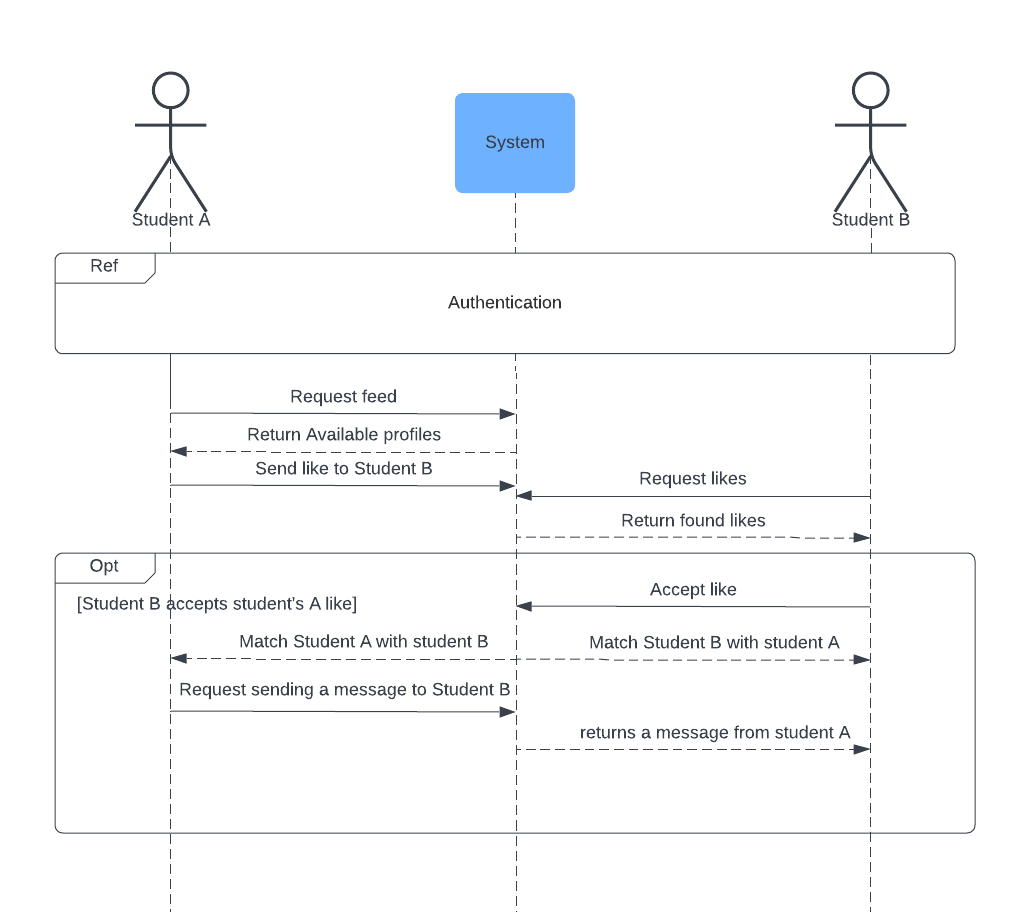
\includegraphics[scale=0.7]{diagrams/Sequence diagram like management.png}
            \caption{Likes management system sequence diagram} 
            \label{fig: Likes management system sequence diagram}
\end{figure}

\section{Realization}
In this section, we describe what has been implemented and how the various components and functionalities identified in this Sprint have been instantiated.

\subsection{Uni-match feed and profiles browsing}

With the User needs in mind, the flow for socializing as well as selecting users to connect with is quite friendly and simple to navigate. from a simple motion which is a swipe. similar to this, users can just swipe right to mean they would like to get connected with the other user or just swipe left to reject the other user. When two users have shown their interest towards each other the system tends to recommend the two users as being fit to be partners and thus they are allowed to-chat.\\

Below, we take a look at the matching feed where the user can swipe on different profiles. \\
\begin{figure}[H] 
            \centering
            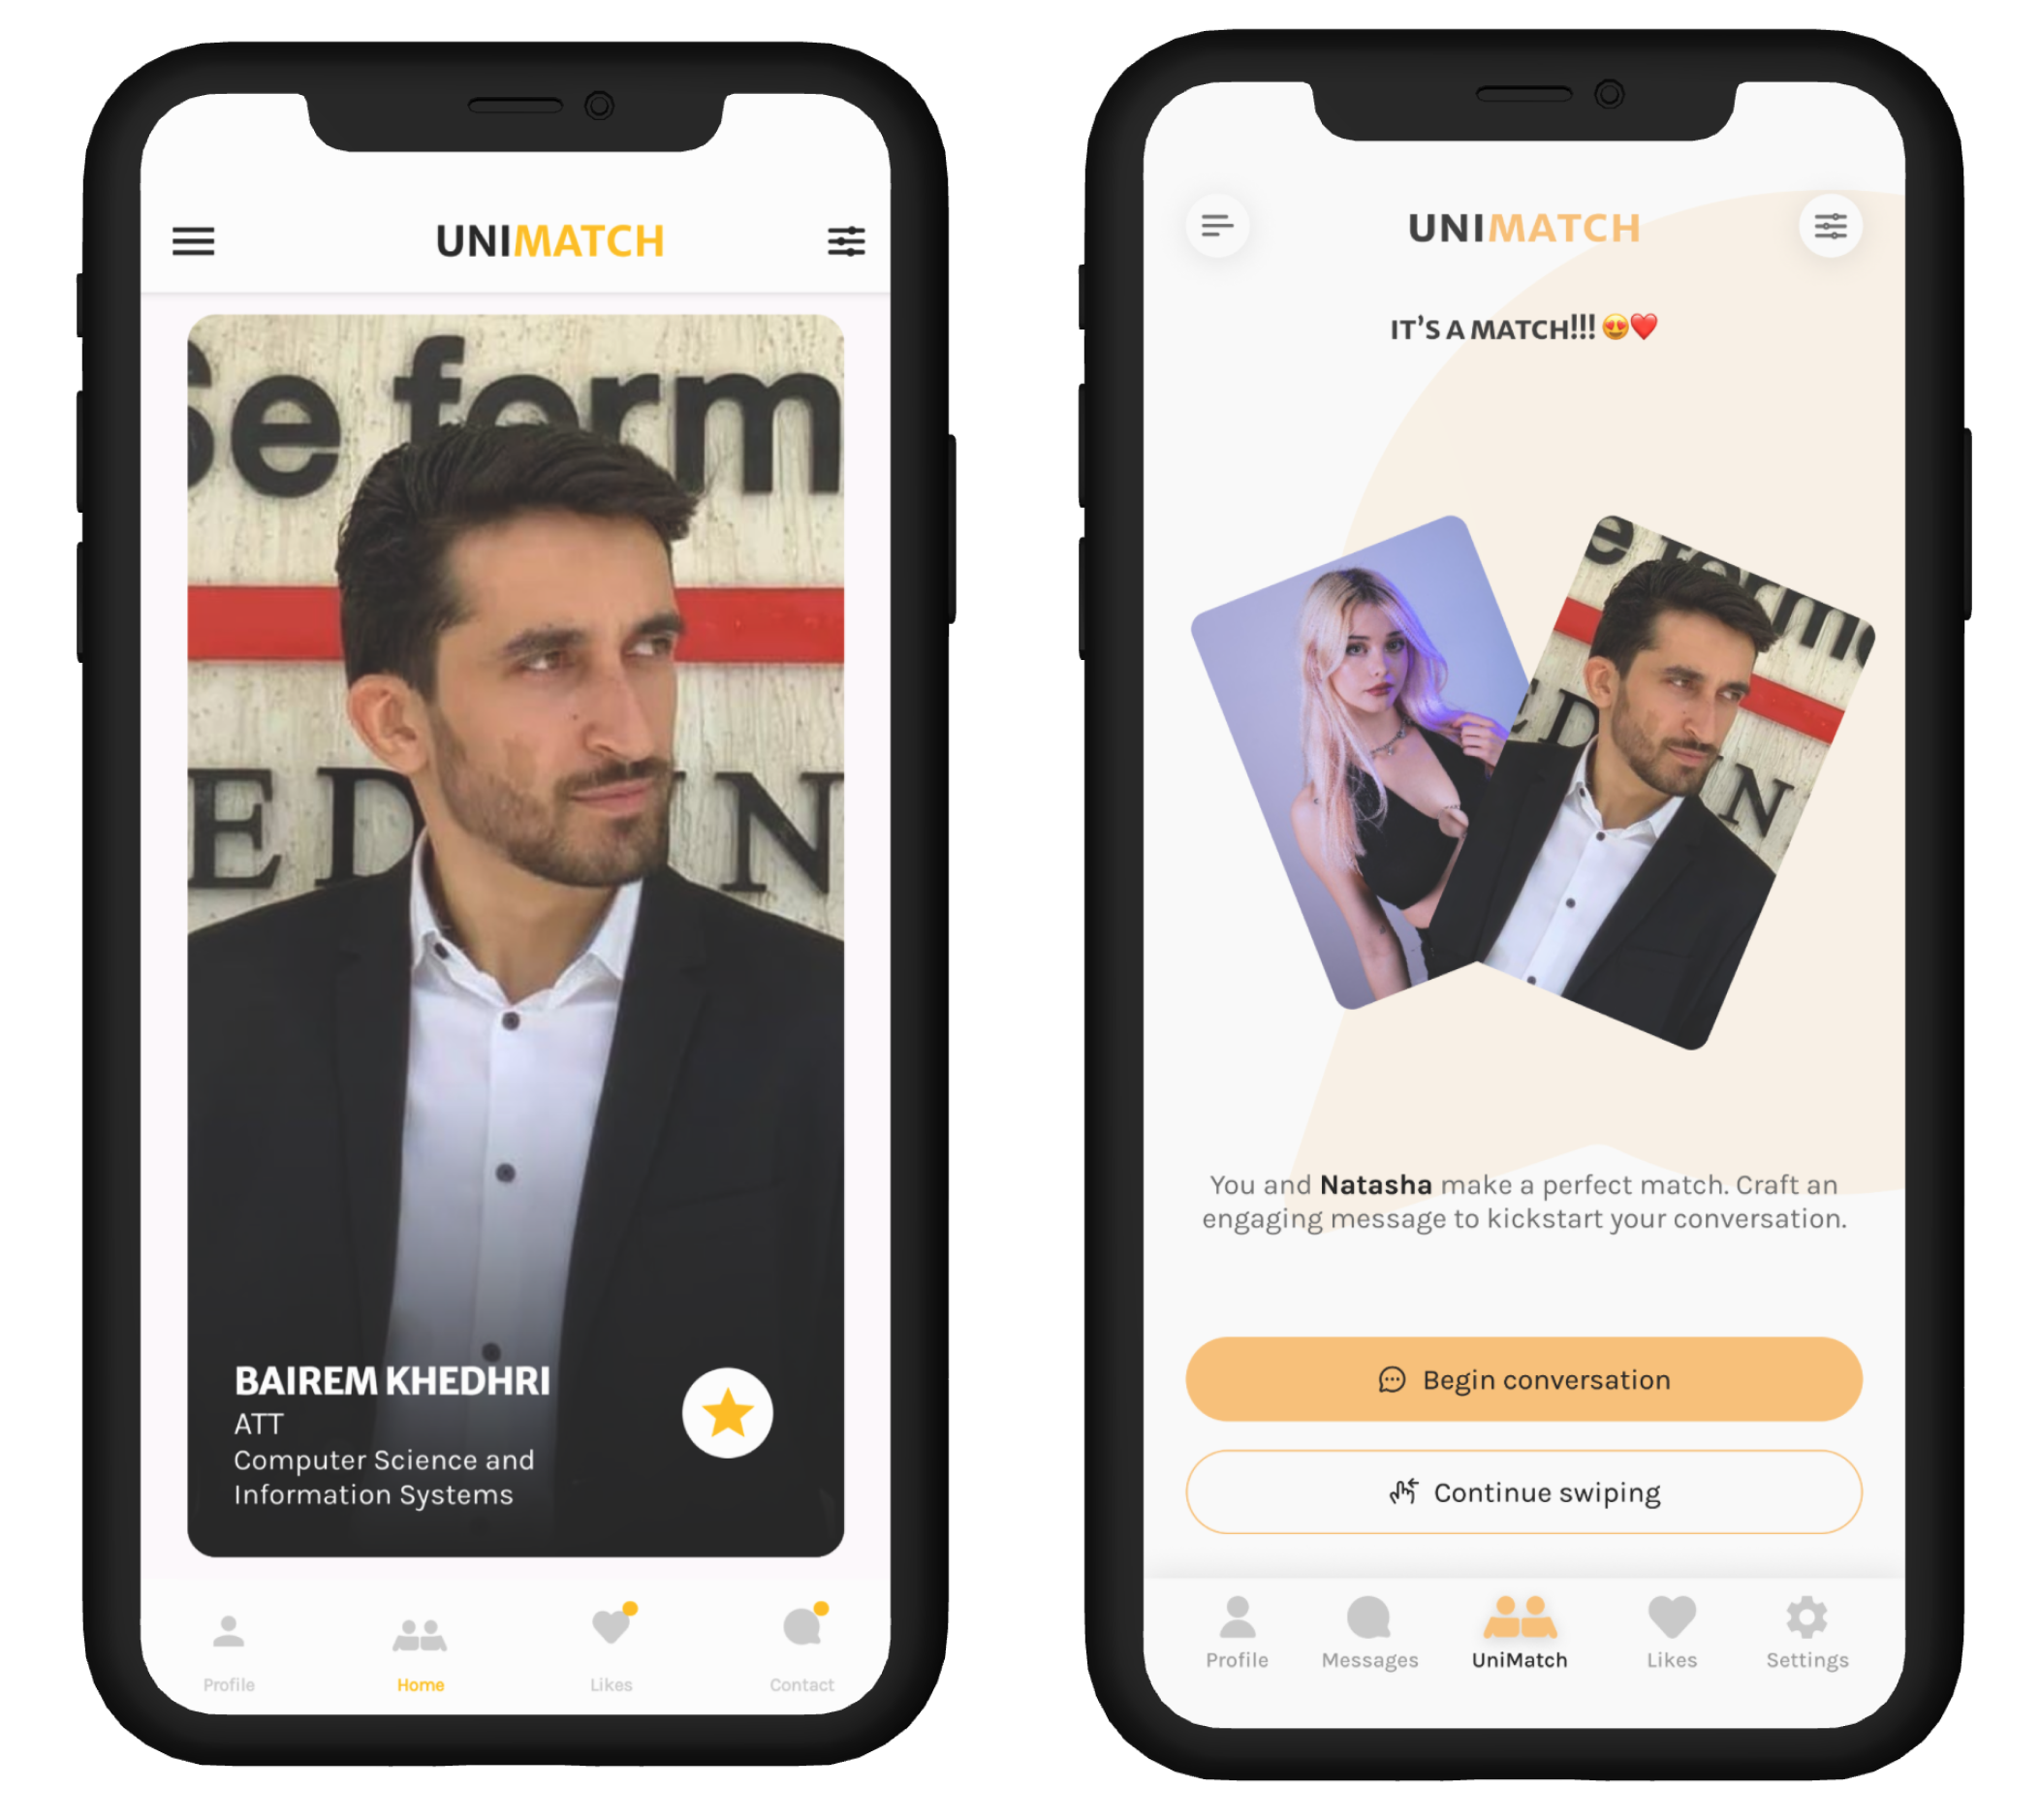
\includegraphics[scale=0.2]{feed ui.png}
            \caption{Some Feed UIs} 
            \label{fig: Feed UI}
\end{figure}

\subsection{Messaging features}
This is as we mentioned above, in the previous sub-section, each time two users match because of the interest they have in each other, they can then send each other a message in the messaging area.

Below this there is the Contacts interface where users can find the list of matches and chats, and to the right we'll find the Chat interface .
\begin{figure}[H] 
            \centering
            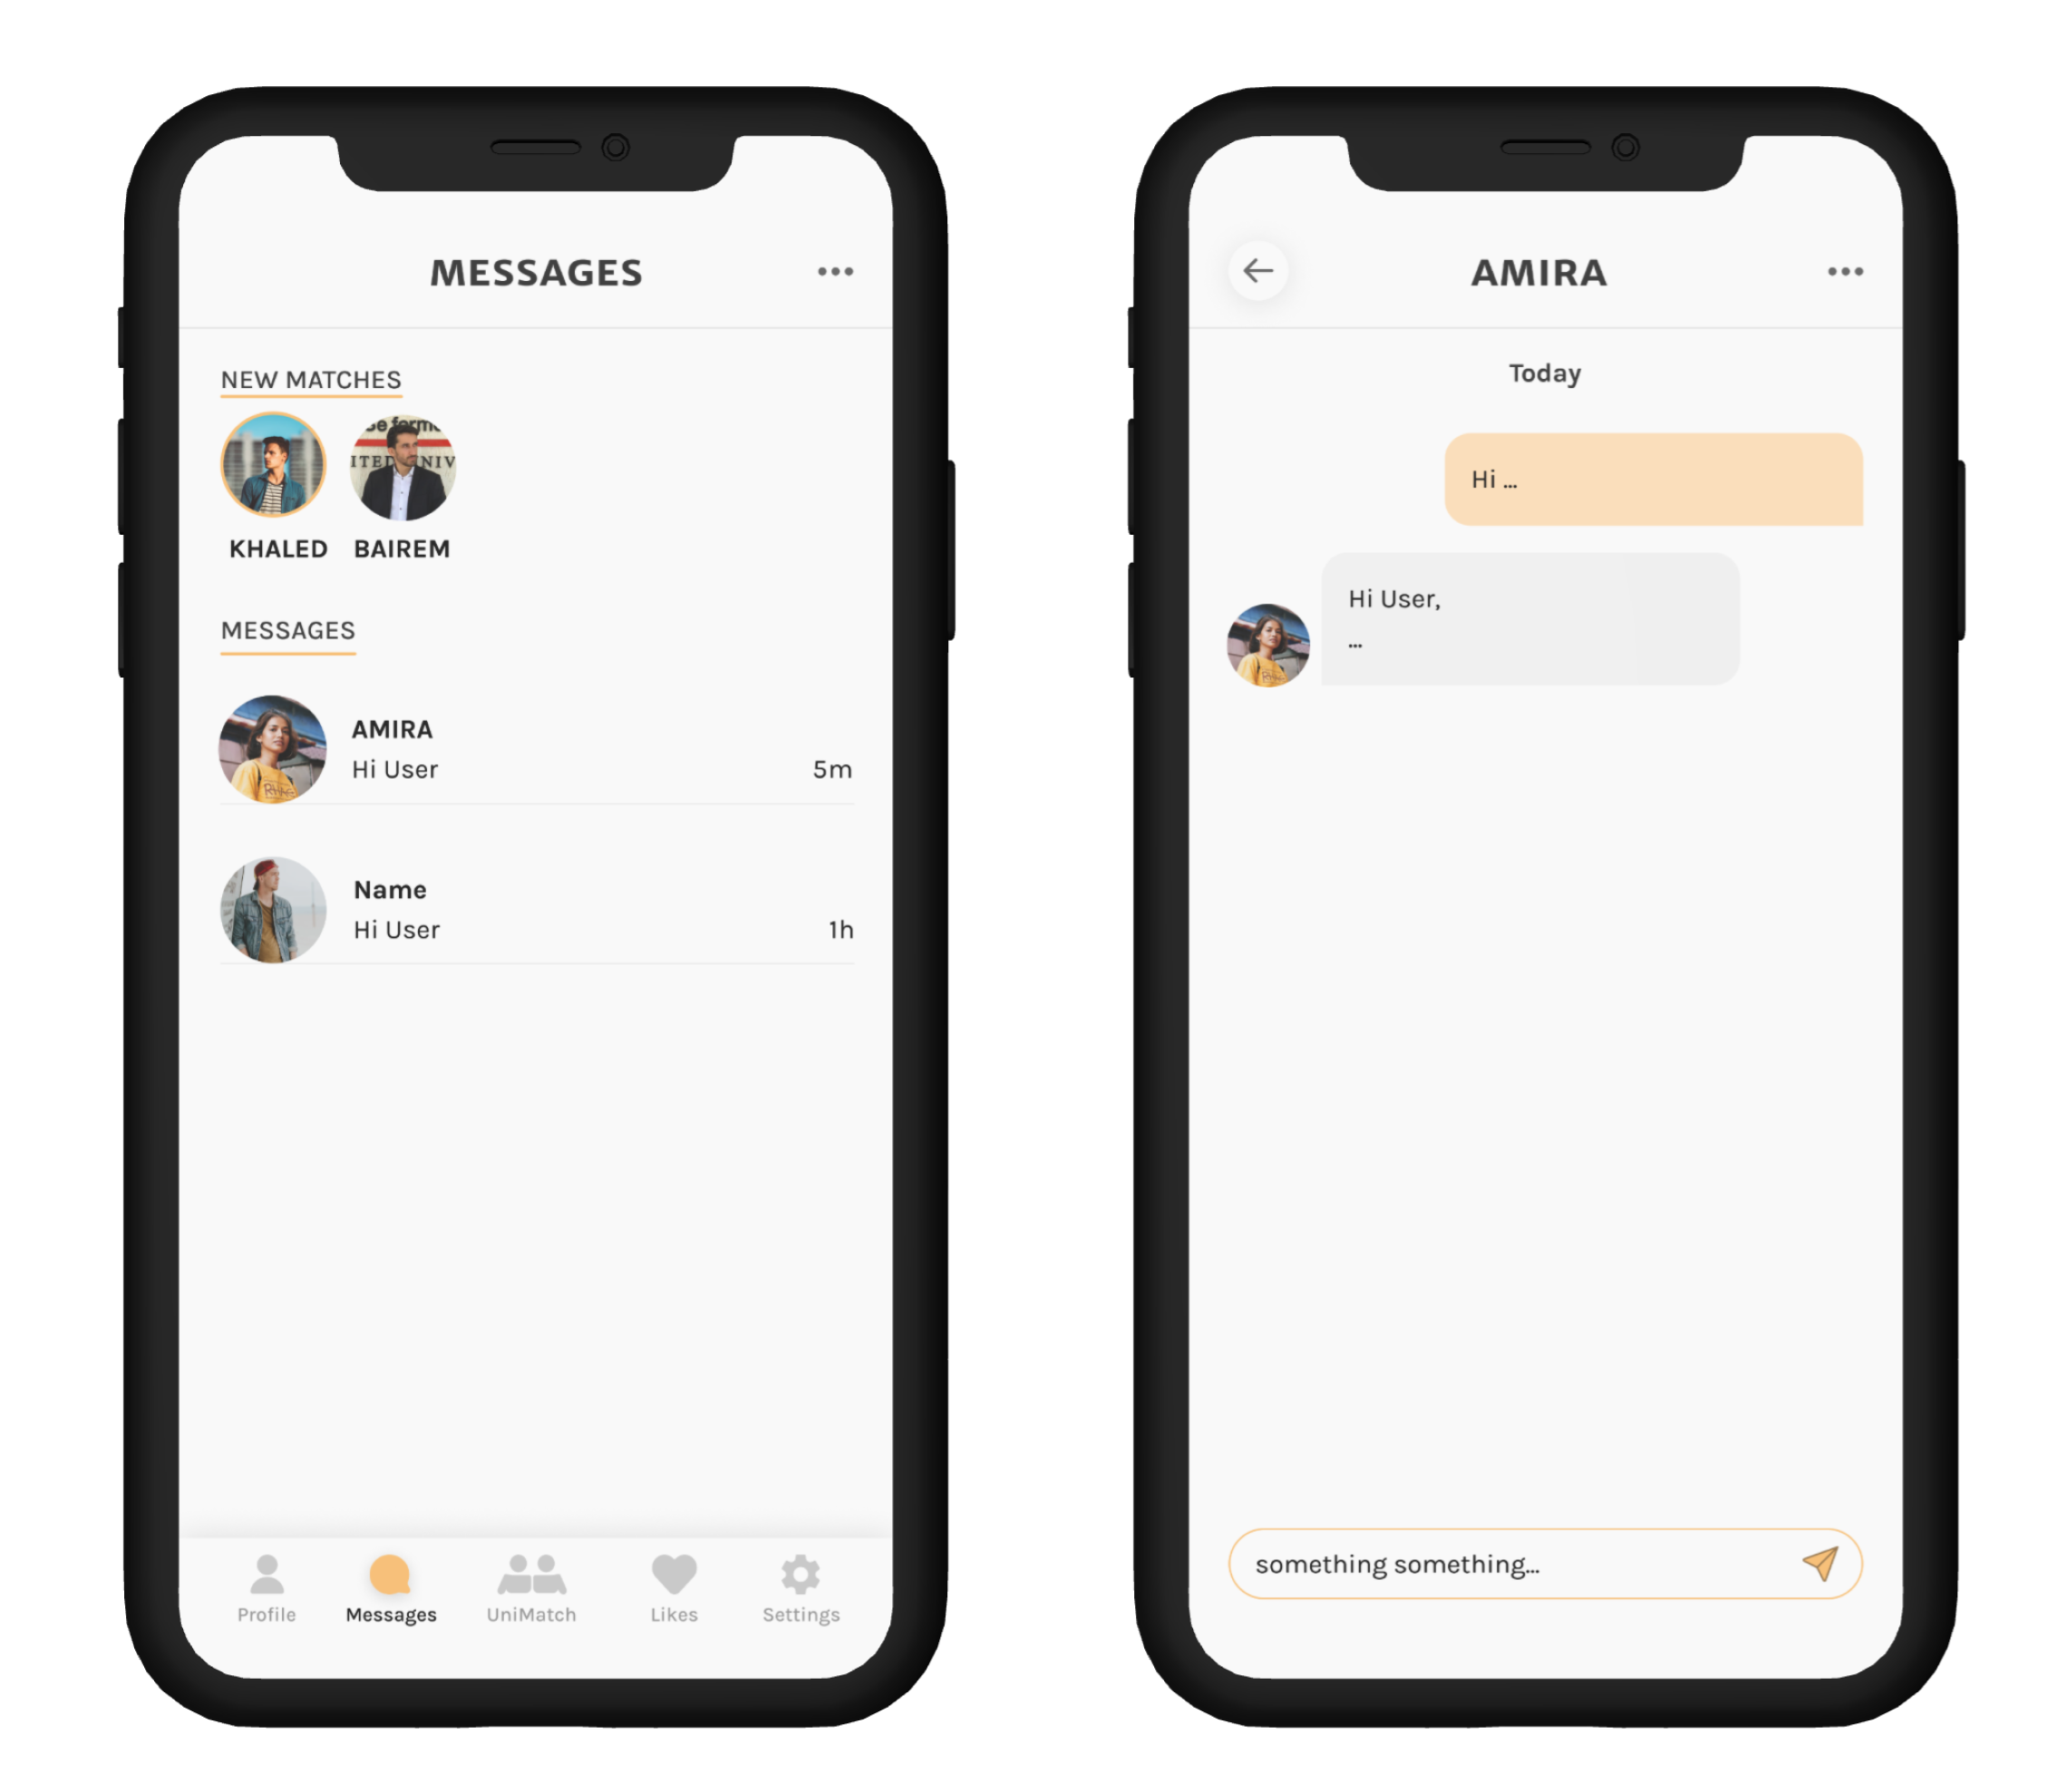
\includegraphics[scale=0.2]{messages ui.png}
            \caption{Messages UI} 
            \label{fig: messages UI}
\end{figure}
\subsection{Likes Management}
After swiping right on a person, they'll notice it in the "Likes" section. In this section, users can guess who likes them by giving them clues about the person who is interested in them. Thanks to these clues, they can find out a little more about the person's personality, which can help them decide whether or not to meet and contact them. \\
In the figure below, we find the "likes" section and on the right- side, we see what happens when we click on one of the "likes" cards to display more details about the person who sent that interest.
\begin{figure}[H] 
            \centering
            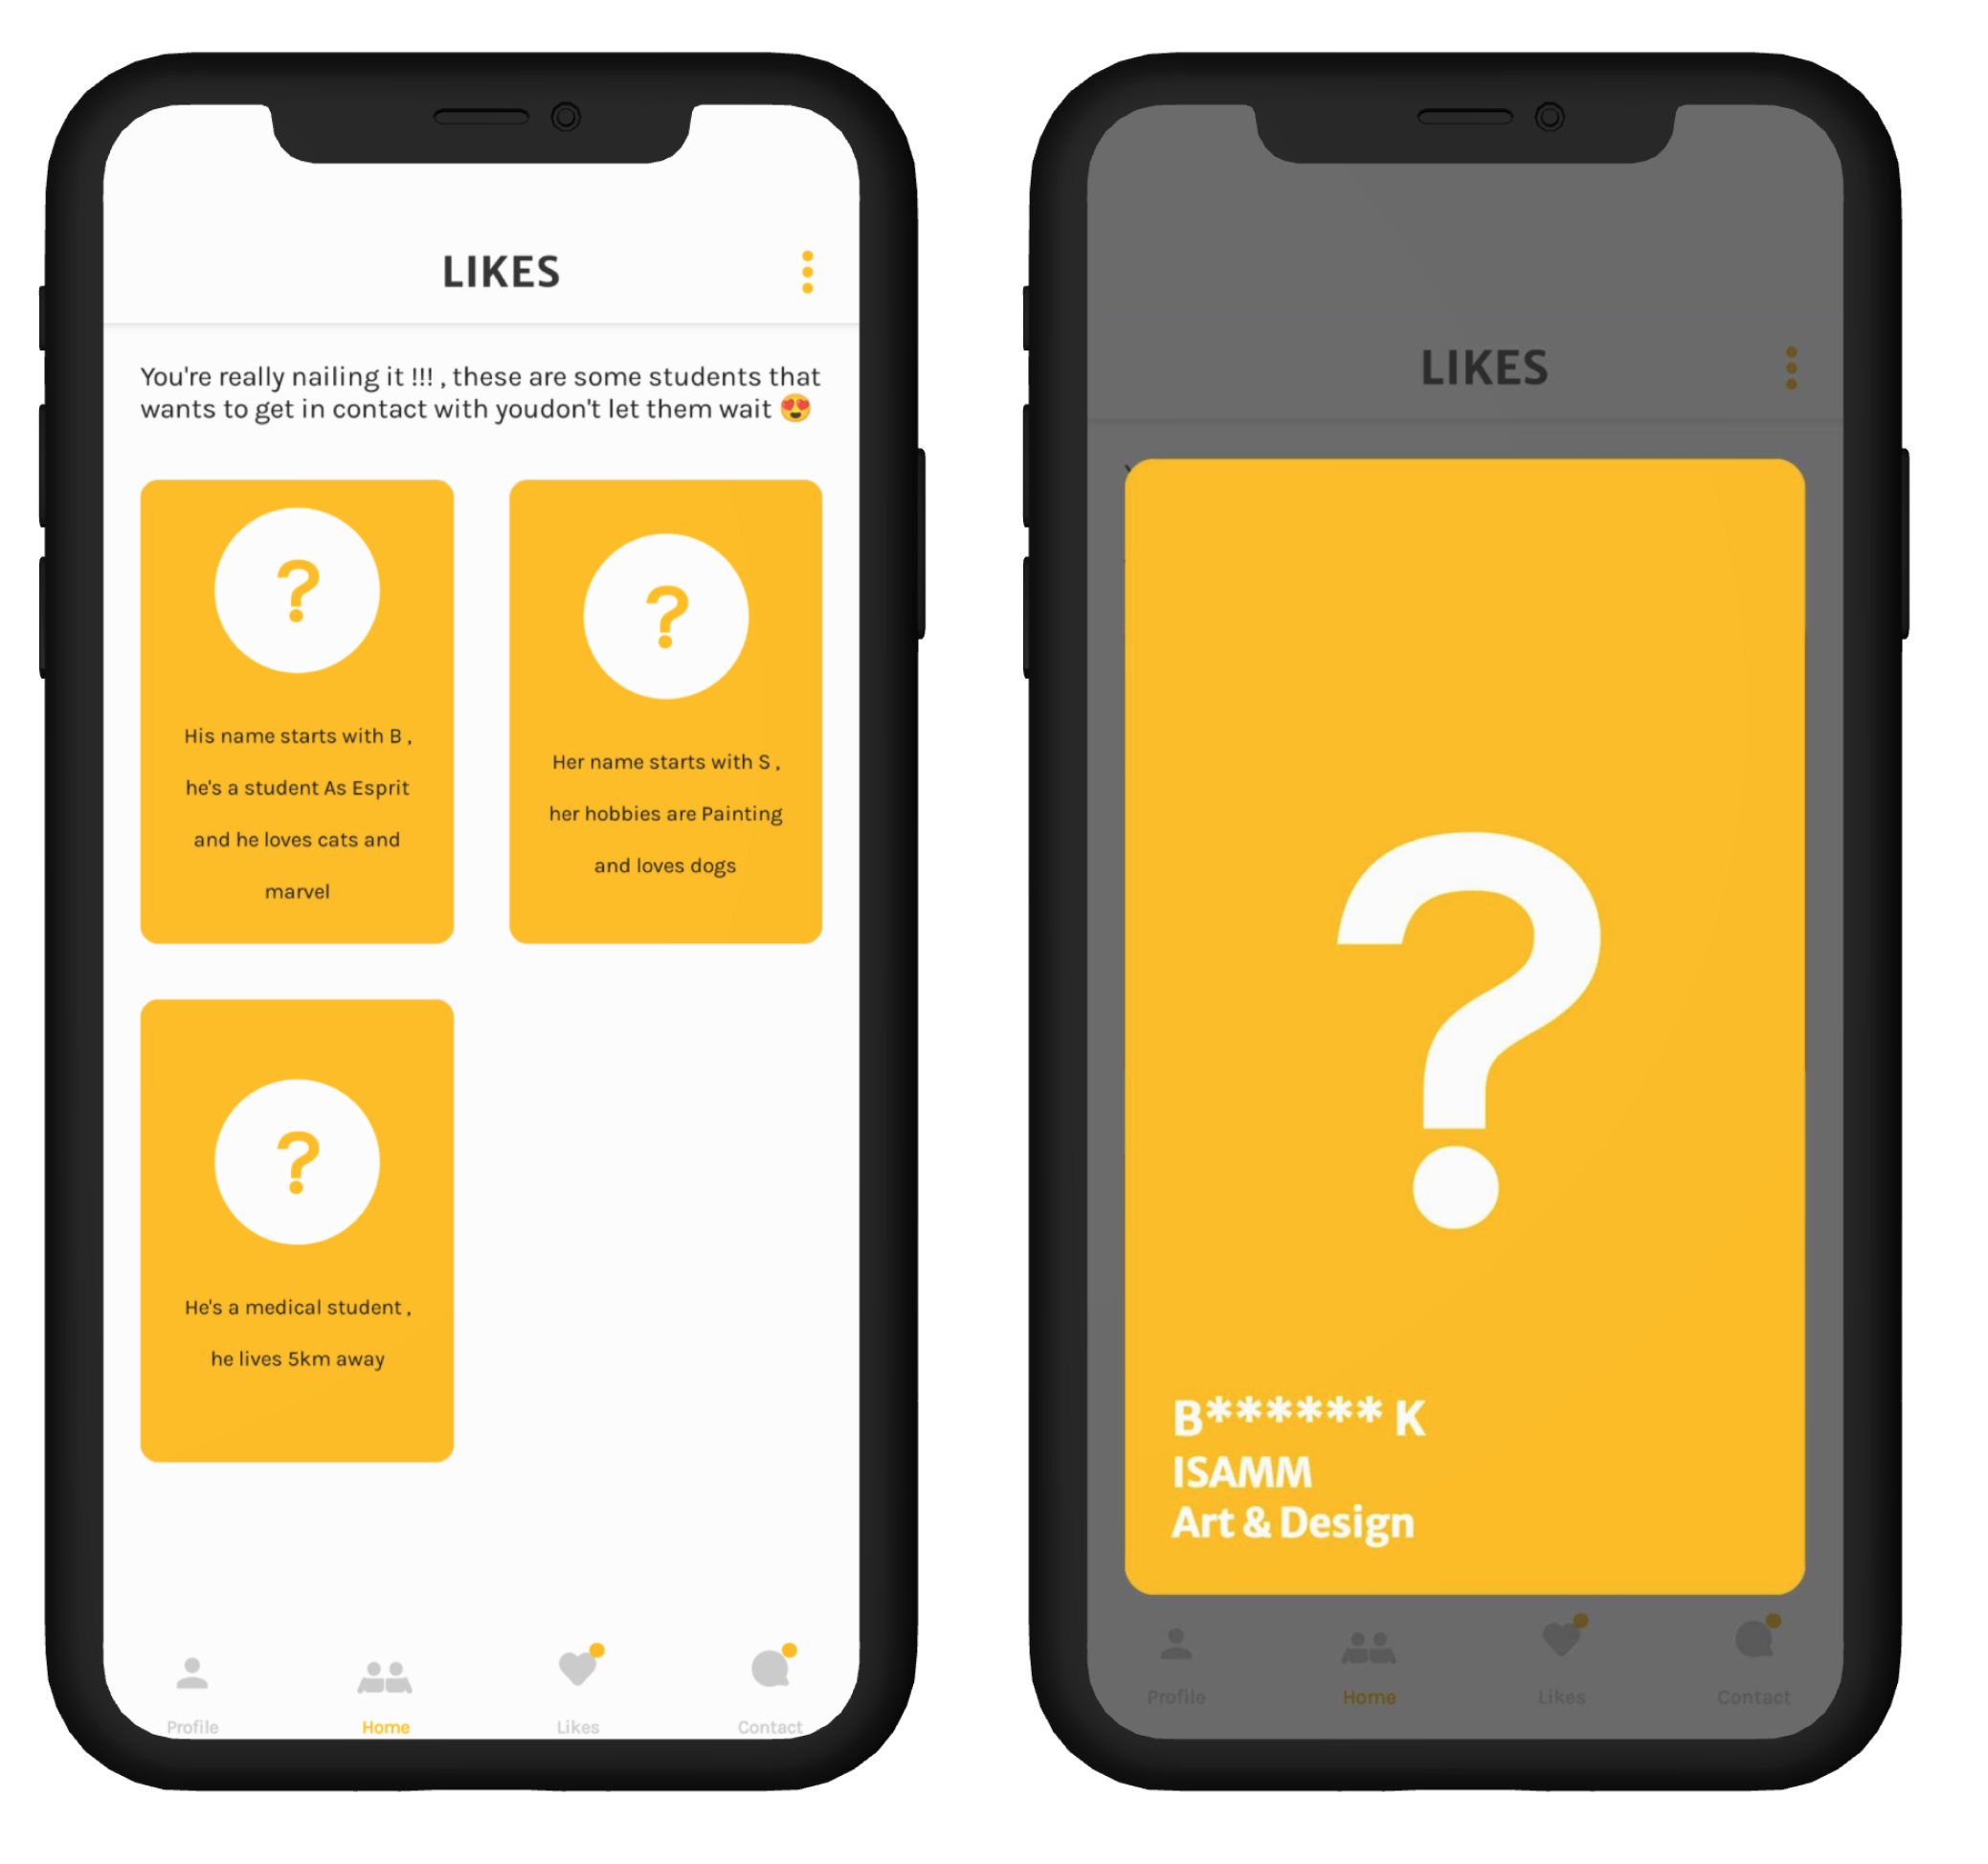
\includegraphics[scale=0.2]{like ui.png}
            \caption{likes management UI} 
            \label{fig: likes management UI}
\end{figure}

\subsection{Filtering Management}
Last but not least, users can choose who they would like to see and have the capability of interacting with them due to a filter option. Users also have a possibility to regulate their potential network with a number of parameters: gender, field of study, university, interests, etc.\\
The following figure is the filtering interface:
\begin{figure}[H] 
            \centering
            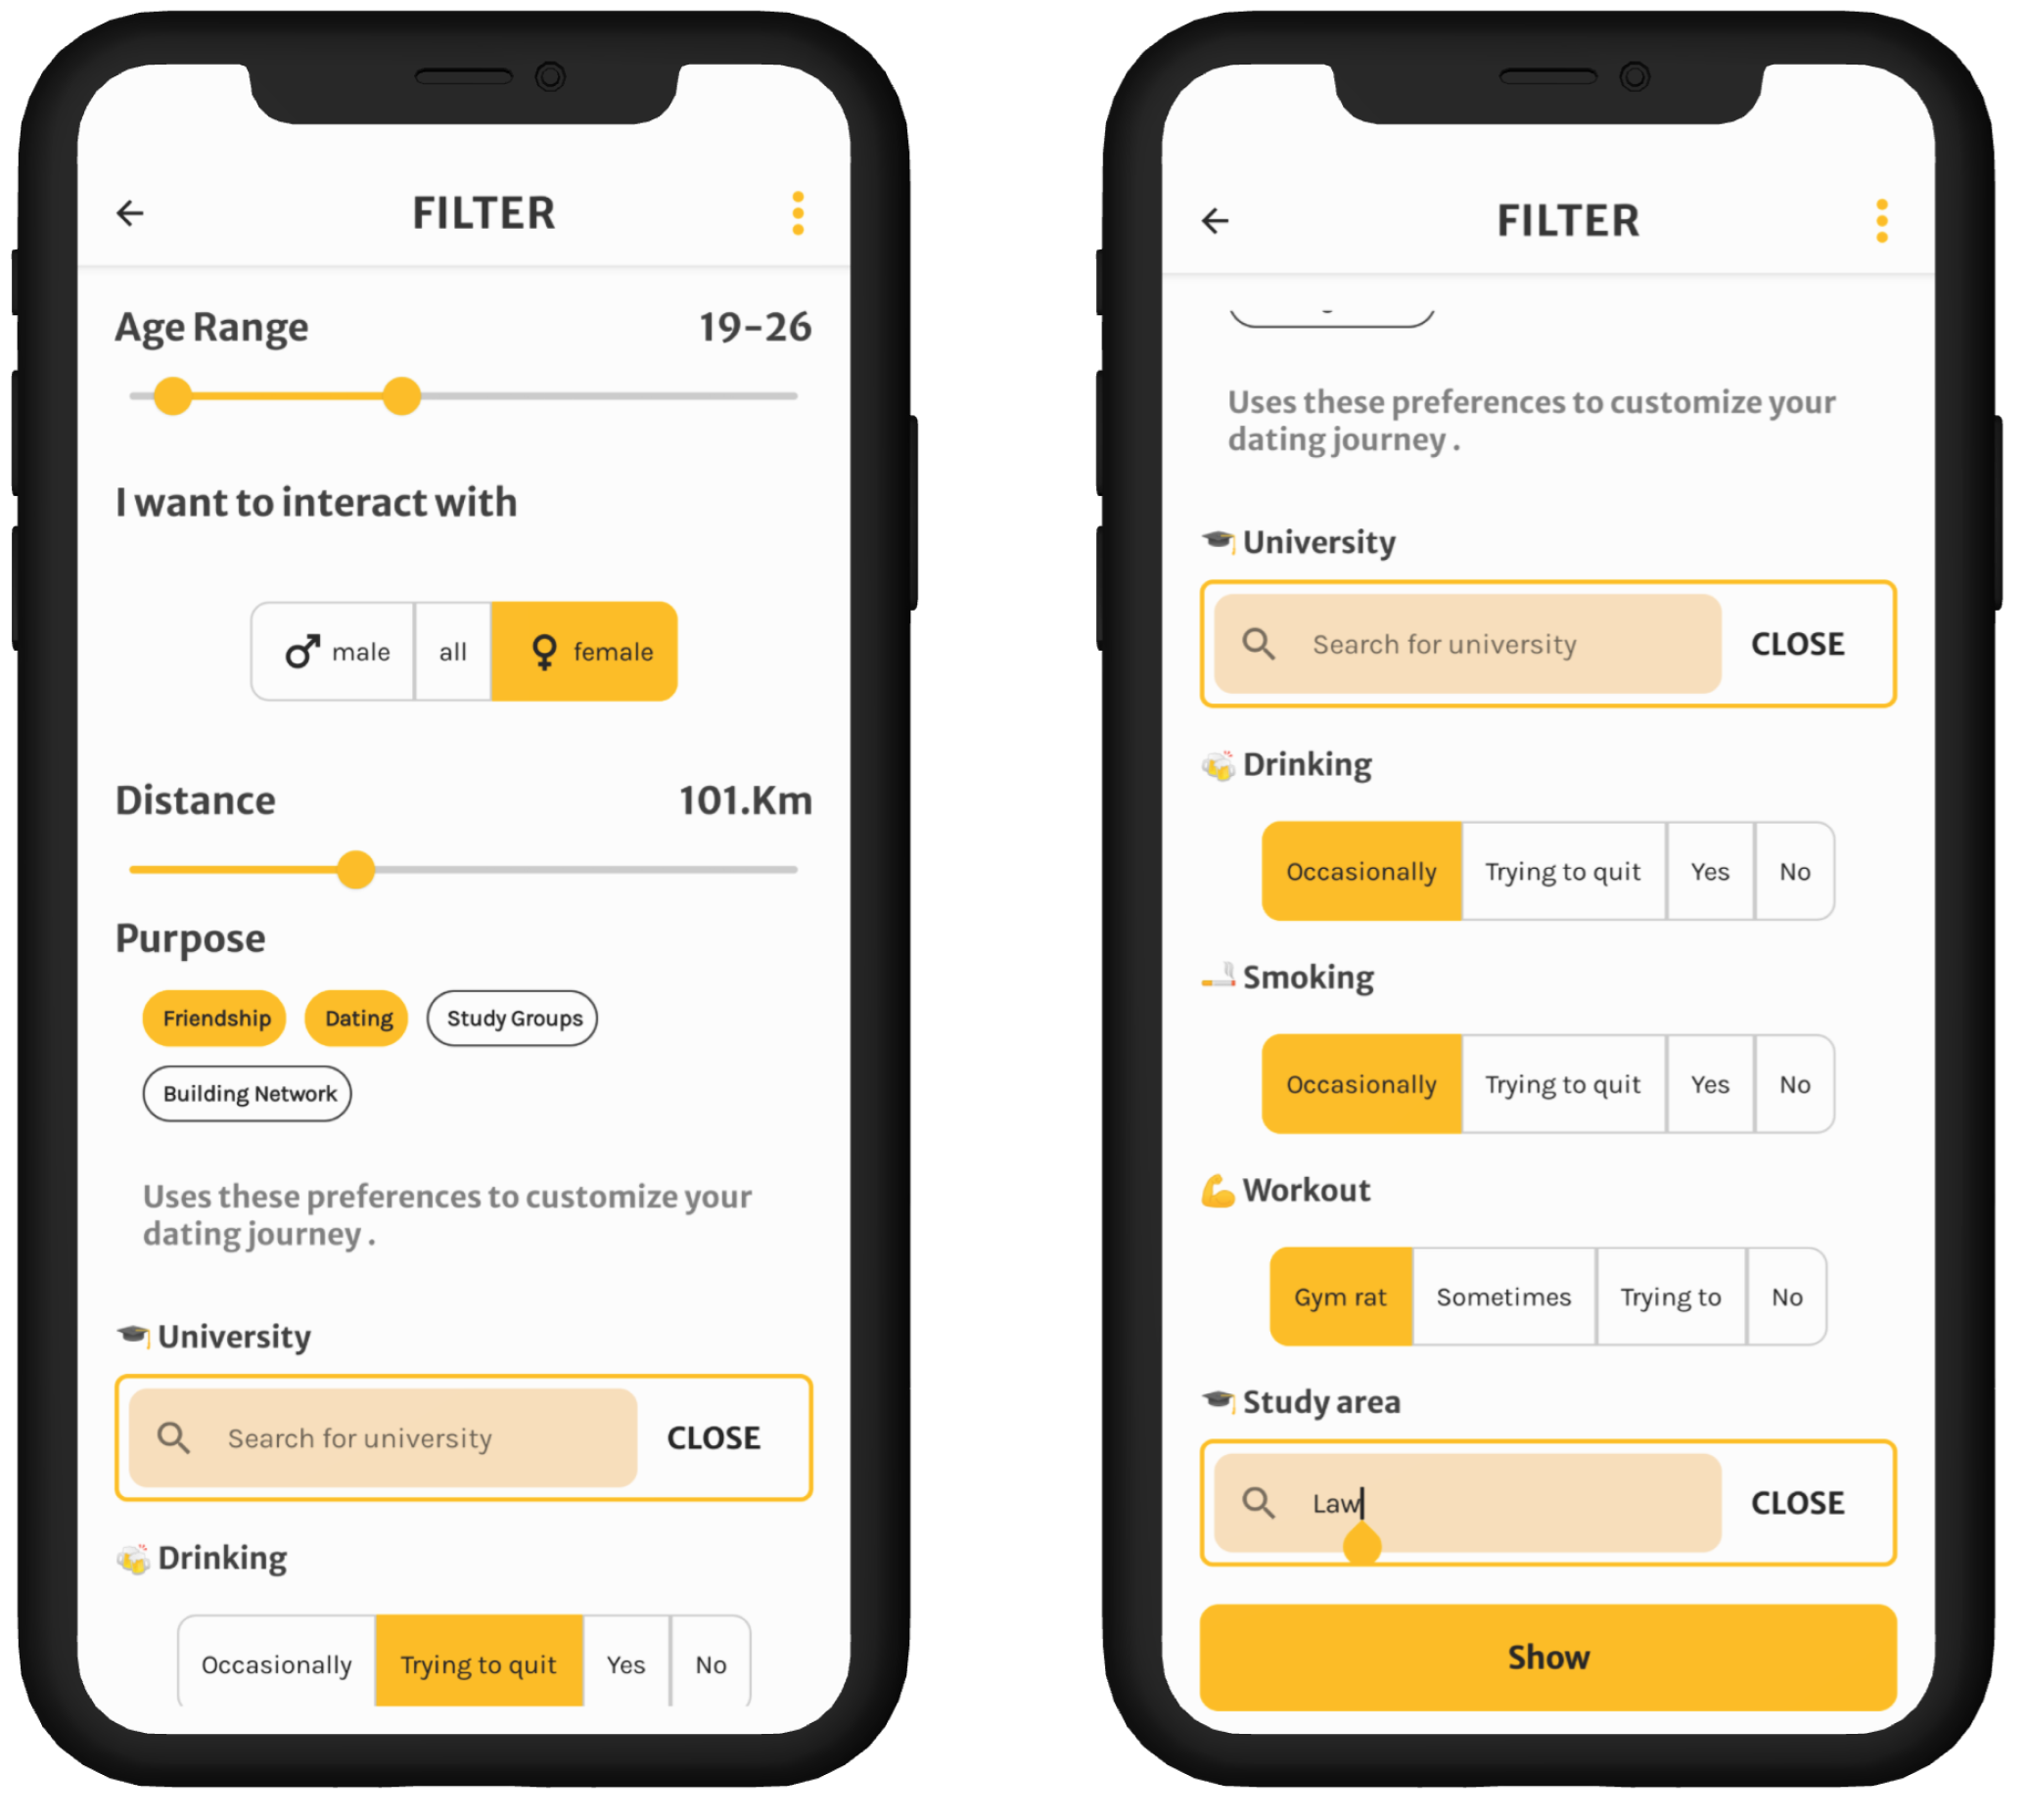
\includegraphics[scale=0.2]{filter ui.png}
            \caption{Feed Filter UI} 
            \label{fig: Feed Filter UI}
\end{figure}

\section*{Conclusion}
\addcontentsline{toc}{section}{Conclusion}
Sticking to the tradition of the chosen methodology, the first sprint introduced a design of the features that are complete for managing users and their authentication. The fact that it is possible to test and specifically these features in the subsequent sprints is the point that brings the team closer to the goal and the great immersive experience. 


\chapter{Sprint 3: Uni-carpool}



\section*{Introduction}

\addcontentsline{toc}{section}{Introduction}

In this chapter, we'll be exploring the last Sprint, which focuses on the design and implementation of uni-world's carppoling features.

\section{Sprint Backlog}
To start, we outline the work to be done in this sprint. The schedule for this iteration
involves the user stories described in the following Table 5.1:

\begin{longtable}{|l|p{6cm}|p{8cm}|}
\hline
ID & User story & Task\\
\hline
\endfirsthead

\multicolumn{3}{c}{{\bfseries}} \\
\hline
Sprint & User story & Task\\
\hline
\endhead

\hline \multicolumn{3}{|r|}{{Continued on next page}} \\ \hline
\endfoot

\hline
\endlastfoot
13 & As a student, I want to browse available carpooling offers & \begin{itemize}
    \item Create the Carpool offer model
    \item Create the algorithm responsible for showing the offers
    \item Create the matching system
    \item Create the Carpool feed UI
    \item Integration and testing
\end{itemize} \\ \hline

14 & As a student, I want to show my interest if I find an offer interesting, and ignore offers I don’t like & \begin{itemize}
    \item Creation of like and dislike features
    \item enhancing the algorithm
    \item Integration and testing
\end{itemize} \\ \hline

15 & As a student, I want to create a carpool offer & \begin{itemize}
    \item Creation of messaging UI
    \item Integration and testing
\end{itemize} \\ \hline

16 & As a student, I want to manage my carpool offers & \begin{itemize}
    \item Creation of the carpool management UI
    \item Integration and testing
\end{itemize} \\ \hline

17 & As a student, I want to see who’s interested in my offers & \begin{itemize}
    \item Creation of likes UI 
    \item Integration and testing
\end{itemize} \\ \hline

18 & As a student, I want to accept or reject other users interested in my offers & \begin{itemize}
    \item enhancing the like and dislike features
    \item Integration and testing
\end{itemize} \\ \hline

19 & As a student, I want to receive notifications when I get a match or message & \begin{itemize}
    \item Creation of notification feature
    \item Integration and testing
\end{itemize} \\ \hline
\caption{Sprint 2 backlog}
\label{Tab: Sprint 2 backlog}
\end{longtable}


\section{ Analysis and conception}
In this section, we illustrate the sprint analysis in a more visual representation using use case diagram for the carpooling features and sequence diagrams of the most highlighted features:
"Offers browsing" and "Offers management".

\subsection{Use case diagram}
\textbf{Refined use case diagram for carpooling features: }
\begin{figure}[H] 
            \centering
            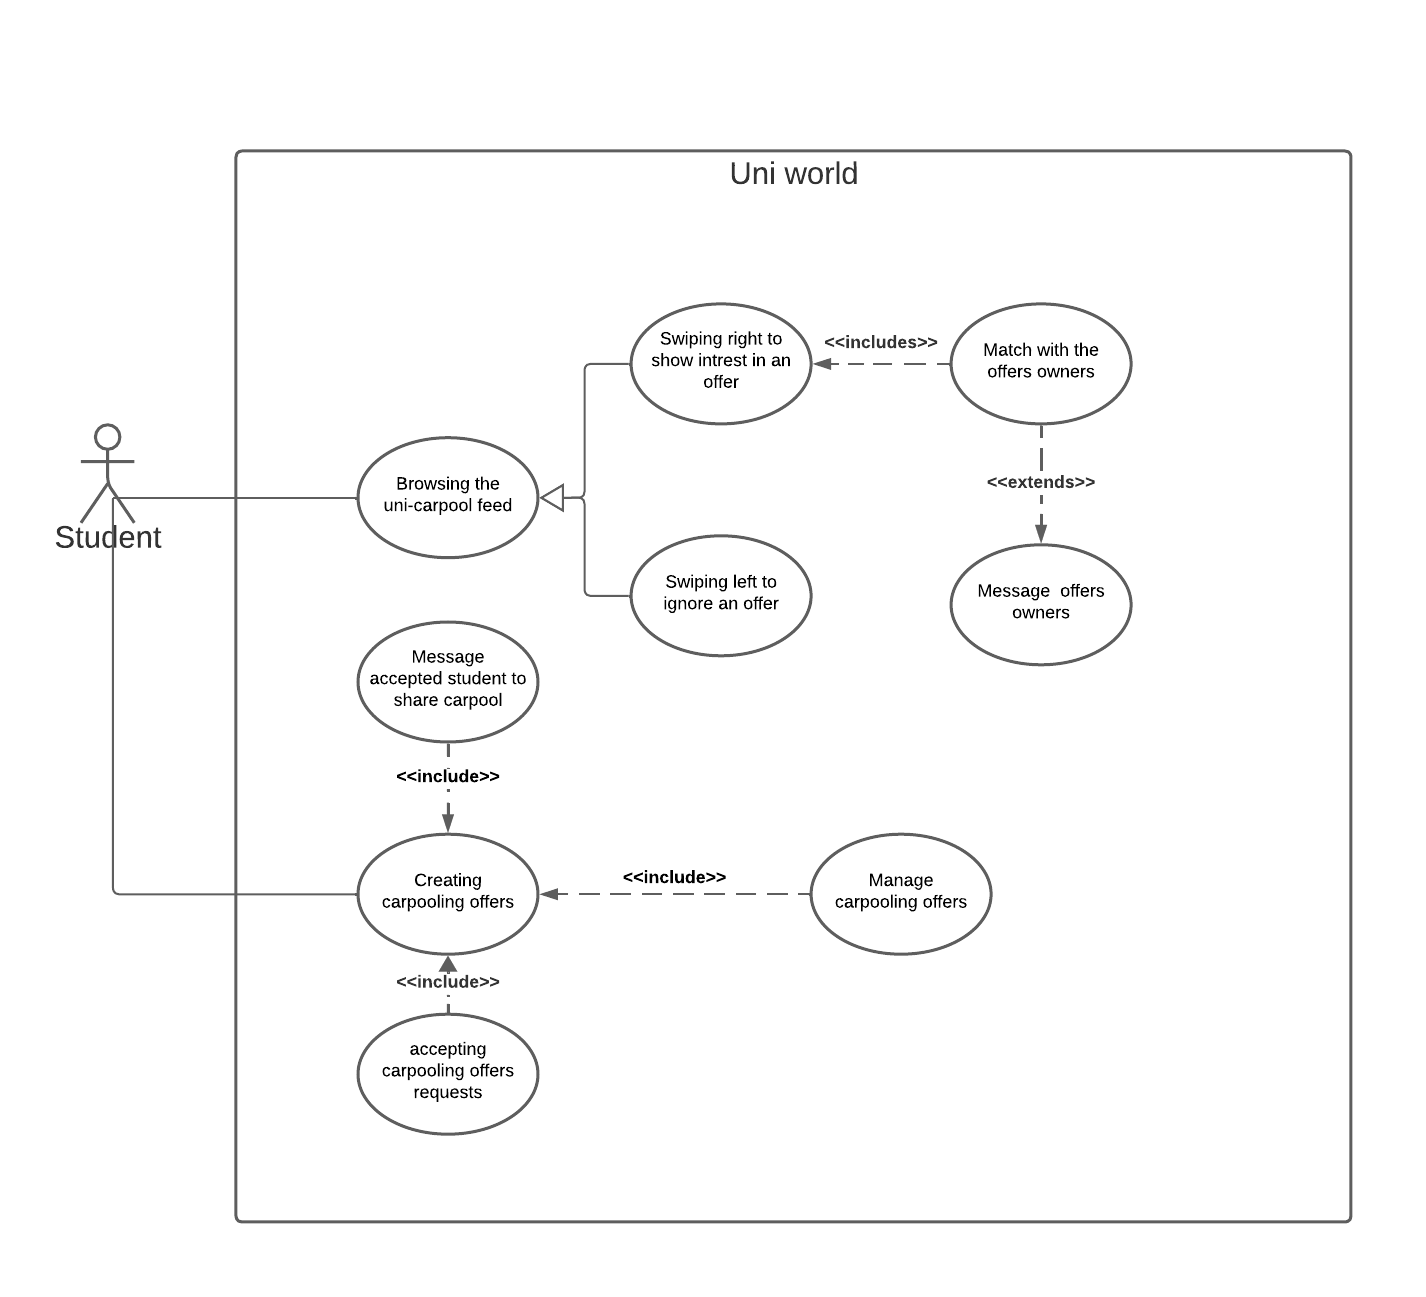
\includegraphics[scale=0.6]{diagrams/refined use case carpool swipe.png}
            \caption{Refined use case diagram for carpooling features} 
            \label{fig: Refined use case diagram for carpooling features}
\end{figure}

\subsection{Use case textual descriptions}
we'll move on to the textual descriptions of the carpooling features such as "Offers browsing" and "Offers management". \\ \\
The offers browsing use case is illustrated in Table 4.2 below:
\begin{longtable}{|c|p{10cm}|}
\hline
Use Case & Description \\\hline
Name & Offers browsing \\\hline
Preconditions & The student must be authenticated and have an active account \\\hline
Post-conditions & once the interest request is accepted by the offer owner, the student and the offer creator match, and a chat will be available to communicate. \\ \hline
Main Flow & 
\begin{enumerate}
    \item After authenticating, the student will get a stack of the offers available in his/her feed.
    \item   Then the student can browse the offer and see information such as the car, the offer owner, the distance between him and the departure place, and both the location of the departure and the arrival places so it helps him/her to choose a suitable offer.
    \item Then the student will have two options:
        \begin{itemize}
            \item   Showing interest in the offer by swiping right on it so that interest can reach the offer owner as a request.
            \item Rejects the offer by swiping left on it to ignore it and move to other options simply.
        \end{itemize} 
        \item The action will be incorporated into the system. 
\end{enumerate}
\\\hline
Alternative Flows & 
    if there is a network error, an error message appears
\\\hline
\caption{Textual descriptions of the Offers browsing use case}
\label{Tab: Textual descriptions of the Offers browsing use case}
\end{longtable}

The use case textual description of "Offers management" is illustrated in the
following Table 3.3:

\begin{longtable}{|c|p{10cm}|}
\hline
Use Case & Description \\\hline
Name & Offers management \\\hline
Preconditions & The student must be authenticated and have an active
account \\\hline
Post-conditions & user A and User B can match if user A likes User B back
\\\hline
Main Flow &
\begin{enumerate}
    \item After logging in, the student will choose to go to the carpool offer management screen.
    \item The student can then browse their offers to see who is interested in them
    \item The student will then have several options
       \begin{itemize}
        \item Accept or reject requests
        \item Modify an offer
        \item Delete an offer
        \item Add a new offer
    \end{itemize} 
\end{enumerate}
\\\hline
Alternative Flows & \begin{itemize}
    \item if there is a network error, an error message appears
\end{itemize}
\\\hline
Non-functional Requirements & \begin{itemize}
    \item The carpooling offers management will have a user-friendly UI
\end{itemize}
\\\hline
\caption{Textual descriptions of the carpooling offers use case}
\label{Tab: Textual descriptions of the carpooling offers use case}
\end{longtable}

\subsection{Sequences diagram}
The carpooling offers browsing object sequence diagram can be observed in Figure 5.3 below:

\begin{figure}[H] 
            \centering
            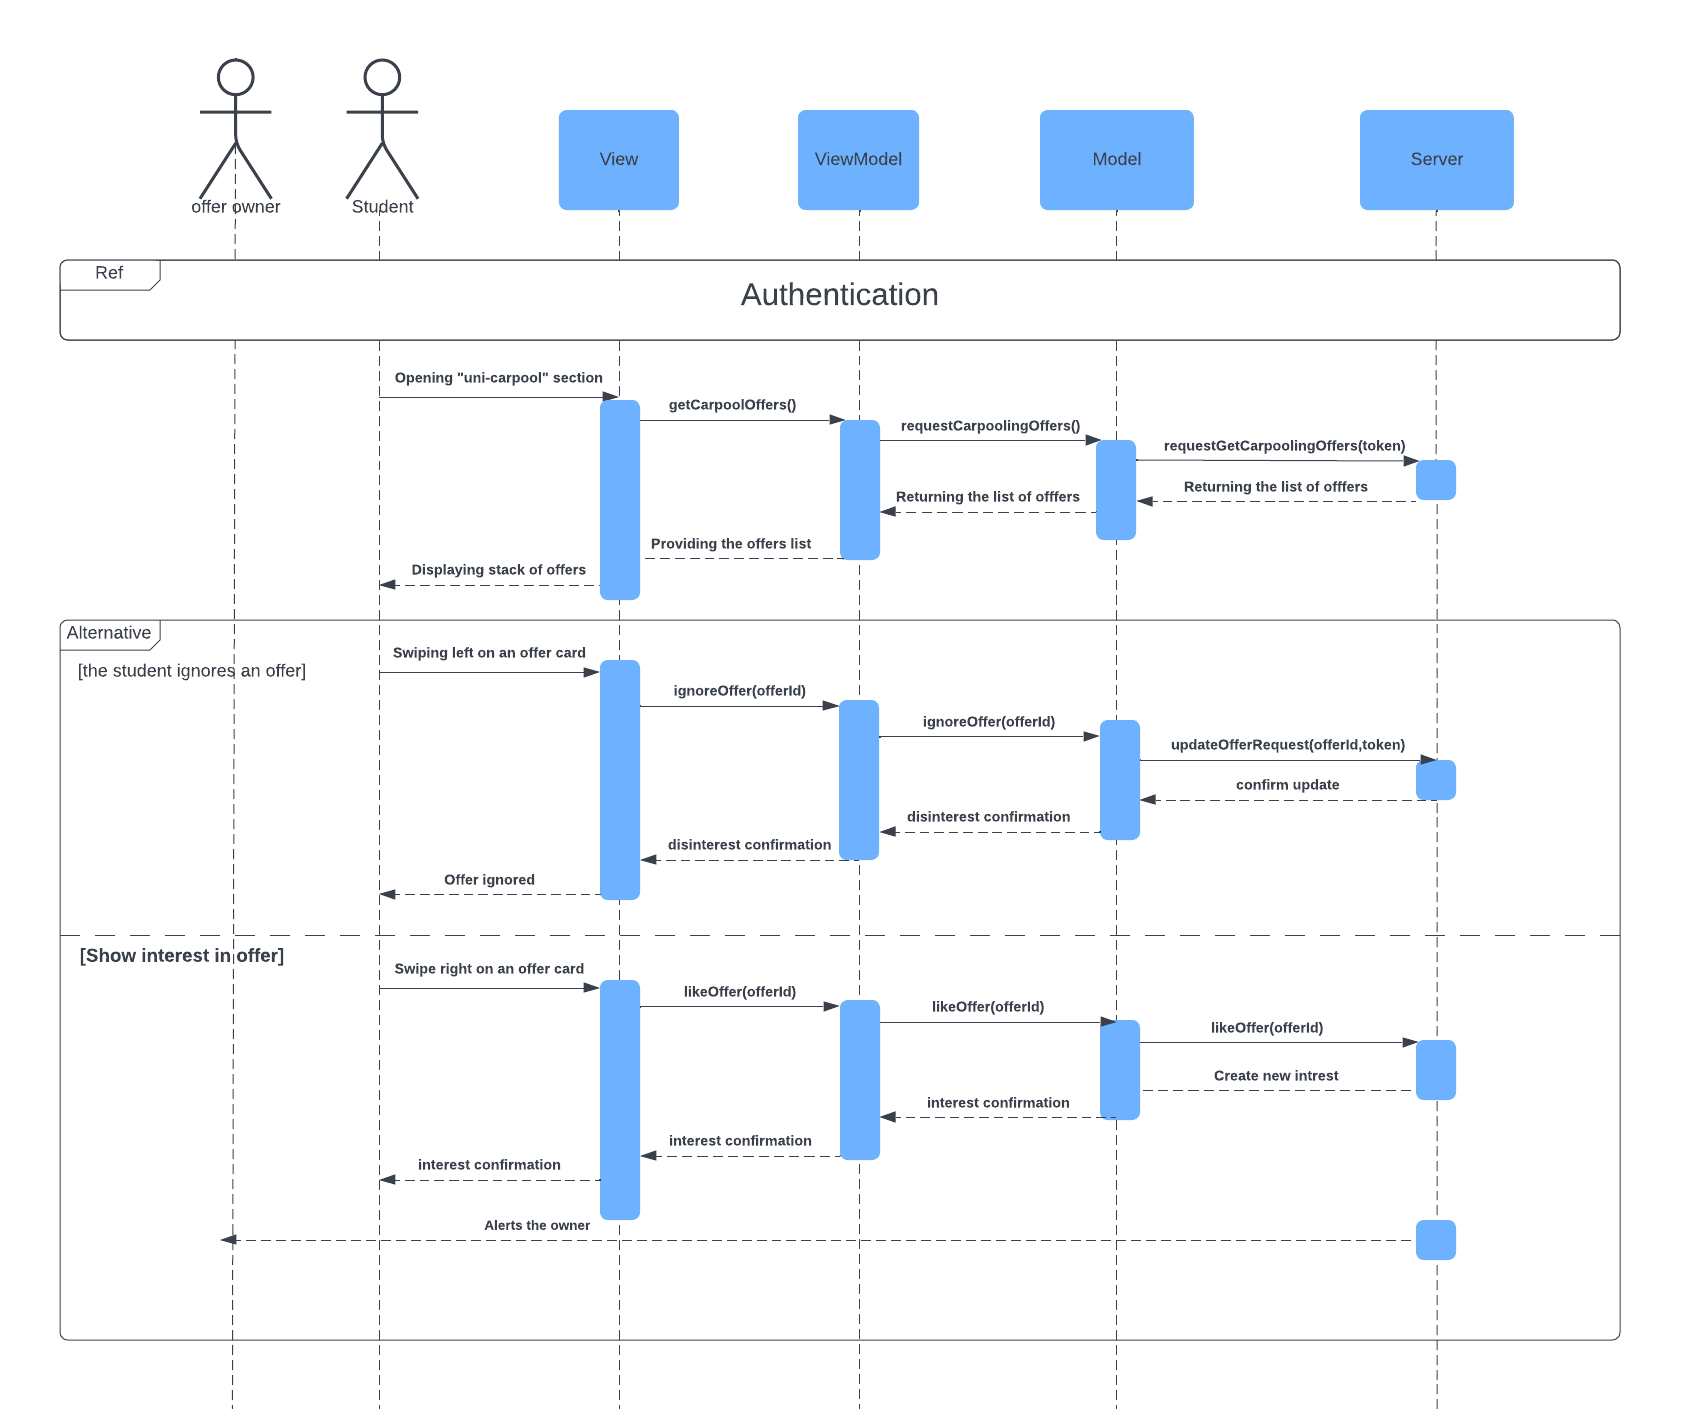
\includegraphics[scale=0.45]{diagrams/Sequence diagram object carpool browsing.png}
            \caption{carpooling offers browsing object sequence diagram} 
            \label{fig: carpooling offers browsing object sequence diagram }
\end{figure}

The adding carpool offers system sequence diagram can be observed in Figure 5.4 below:

\begin{figure}[H] 
            \centering
            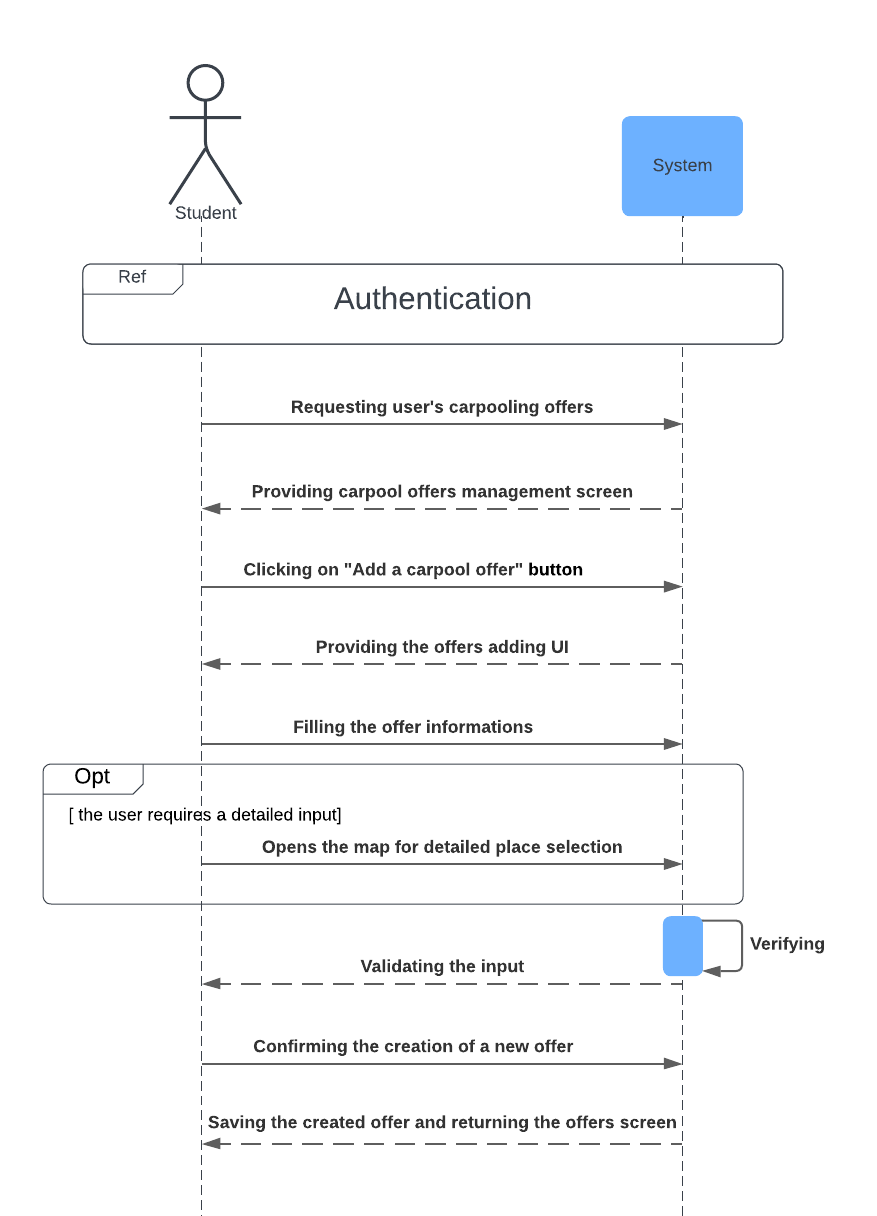
\includegraphics[scale=0.5]{diagrams/Sequence diagram system add carpool offer.png}
            \caption{Add new carpool offer system Sequence diagram } 
            \label{fig: Add new carpool offer system Sequence diagram}
\end{figure}

\section{Realization}
In this section, we describe what has been implemented and how the various components and functionalities identified in this Sprint have been instantiated.

\subsection{Uni-carpool feed and offers browsing}

After taking the user's needs into account, he or she will have a feed full of carpooling offers to choose from, and the user interface will be easy and fun to use, requiring only two main behaviors: scrolling, and swiping. scrolling in this context gives the user the detail view of the offer; and swiping that gives the user the gesture to show interest or ignore the offer.\\

Below, we take a look at the feed where the user can swipe on different offers. \\
\begin{figure}[H] 
            \centering
            \includegraphics[scale=0.1]{ui/unicarpool feed ui.png}
            \caption{Some Uni-carpool feed UIs} 
            \label{fig: Uni-carpool feed UIs}
\end{figure}

\subsection{Adding offers}
Any user can add a new carpool offer, uni-carpool provides an easy-to-use process for adding an offer by submitting details such as departure and destination locations, the price of the journey if the user wishes to earn extra money, the estimated arrival time as well as a description so he can talk more about the offer and finally he can put photos related to the journey to attract other users and make his offer noticeable. \\
In the figure below, we take a look at how we can add a carpooling offer showing the UIs where the user can add his offers
\begin{figure}[H] 
            \centering
            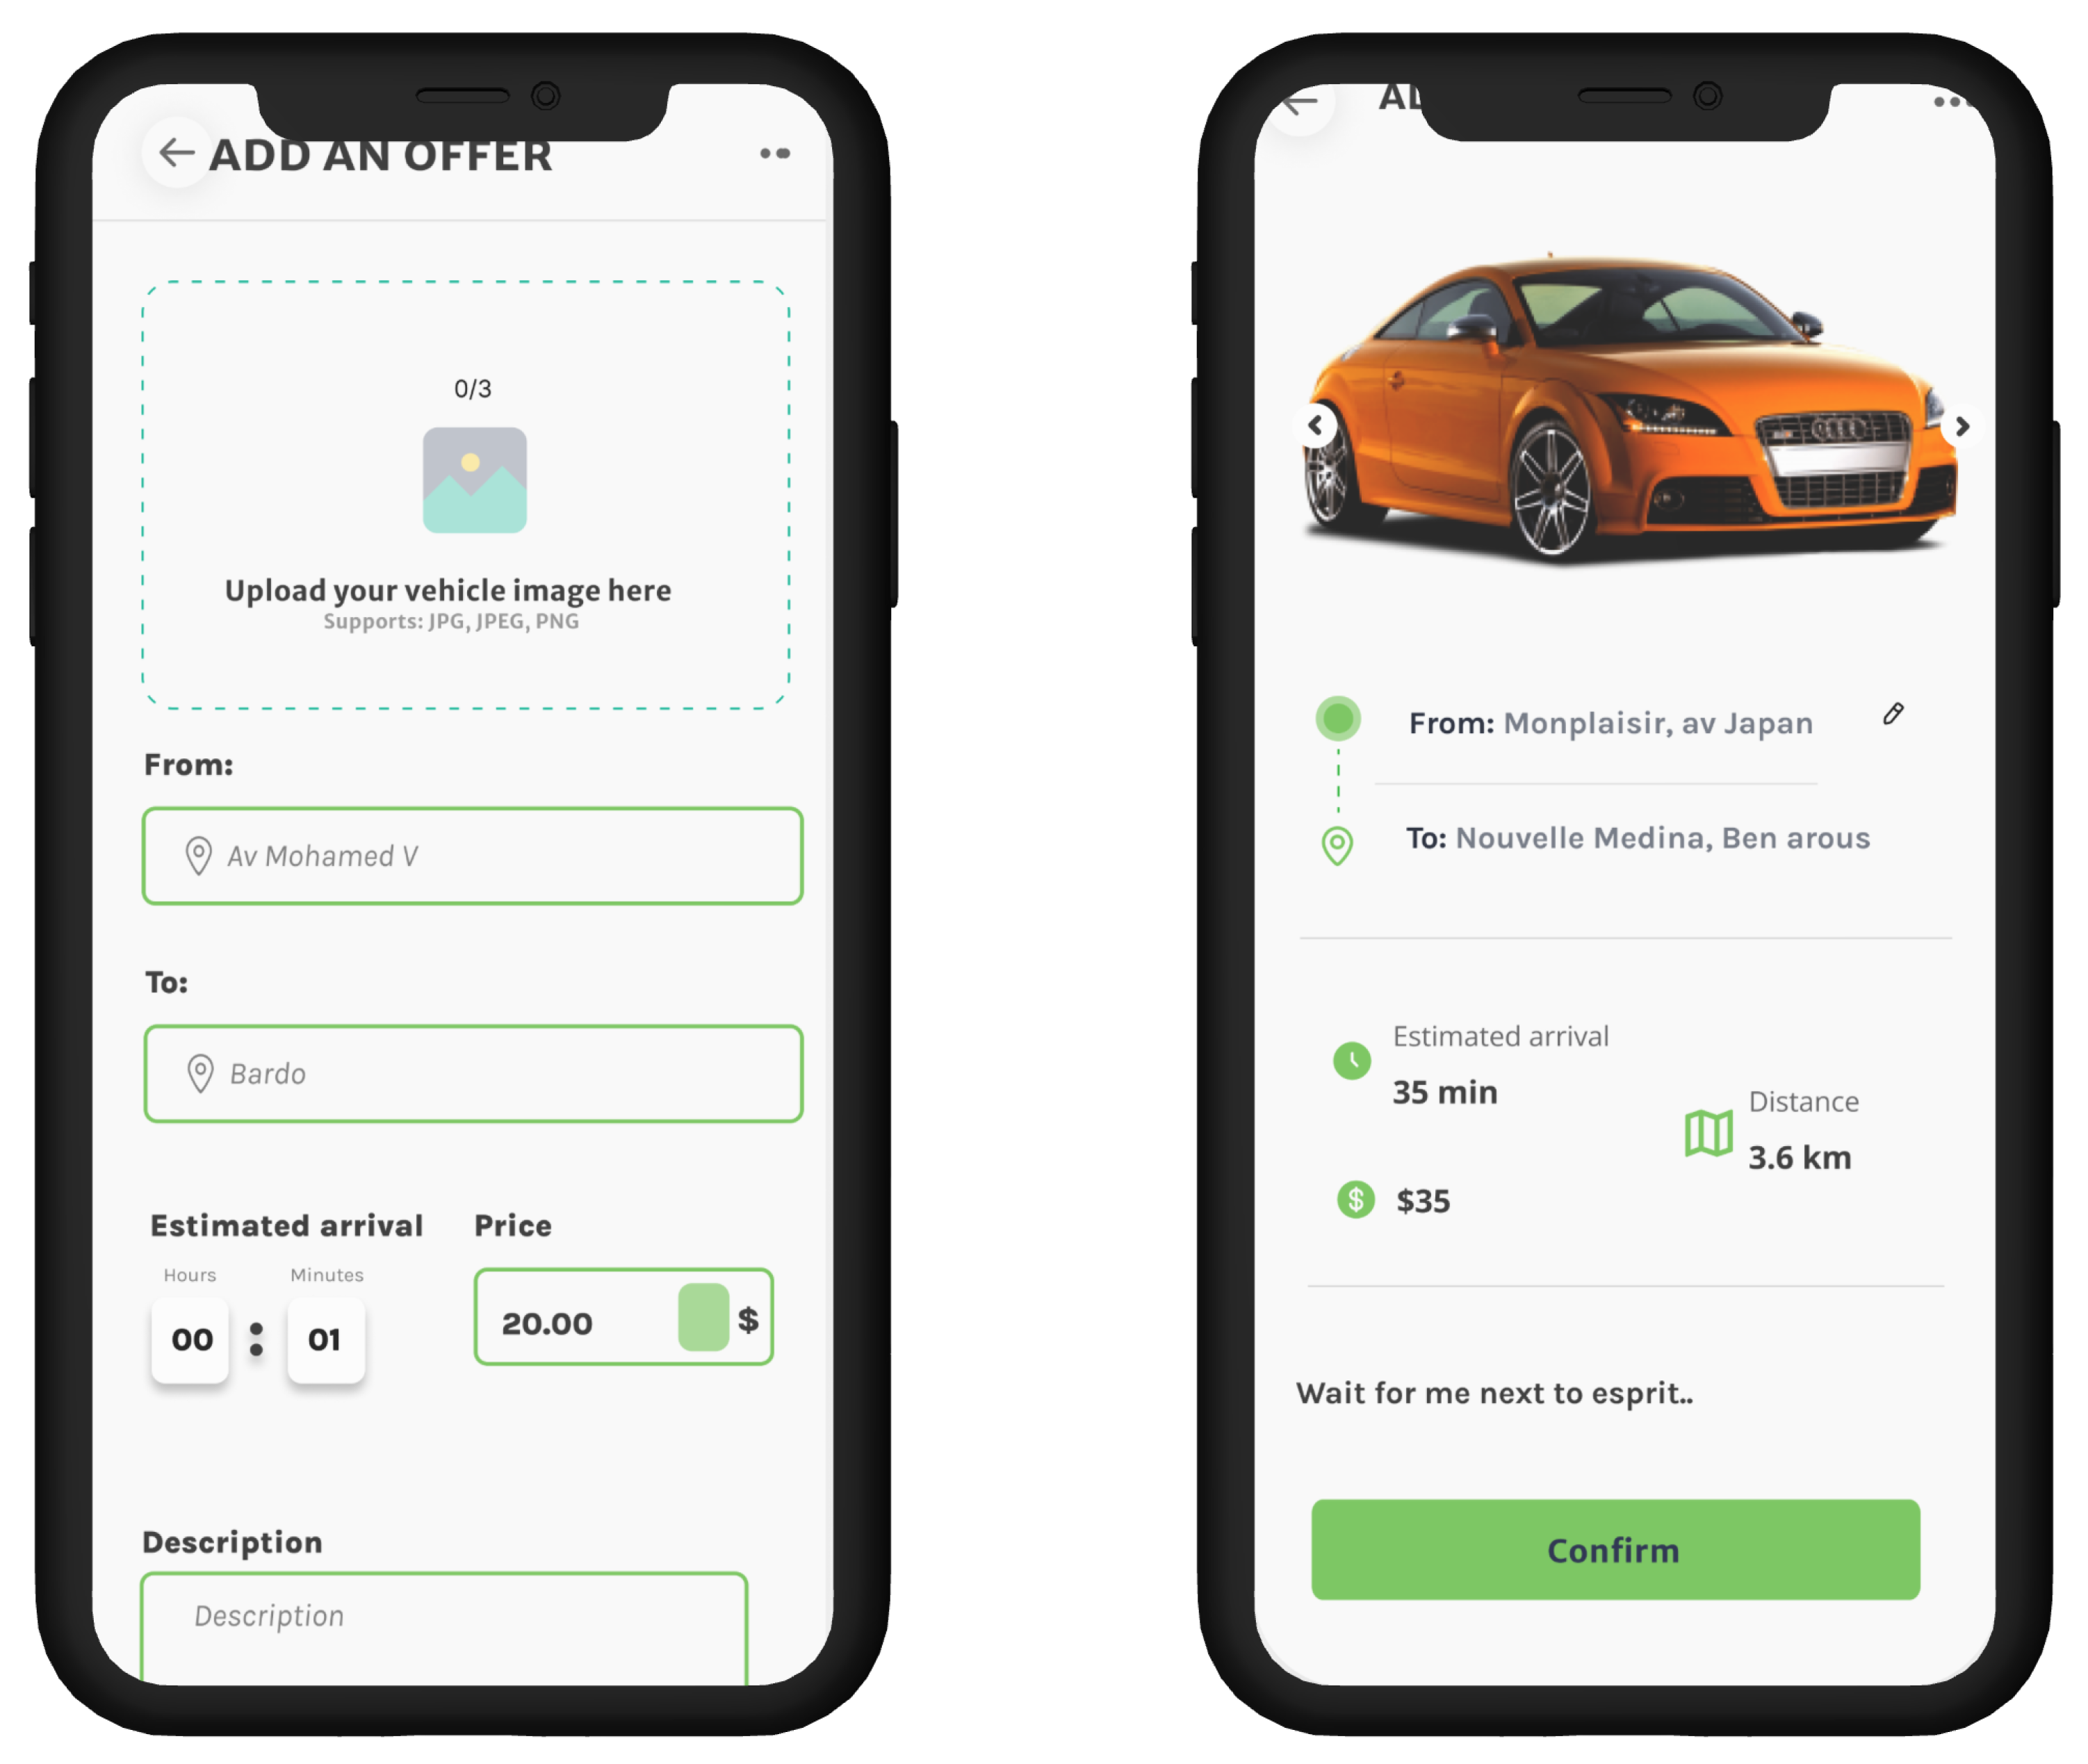
\includegraphics[scale=0.15]{ui/adding carpooling offer.png}
            \caption{Adding carpooling offer feature} 
            \label{fig: Adding carpooling offer feature UI}
\end{figure}

\subsection{Offers management}
What happens after right swiping according to the suggested algorithm is that after right swiping on an offer, the owner of that offer, that is the person who created the offer will notice it in the “Offer management” section. Here users can view the details of people who expressed an interest of their various offers and either approve or deny the request. \\
In the figure below, we take a look at the carpooling offers management screen where the user can manage his offers
\begin{figure}[H] 
            \centering
            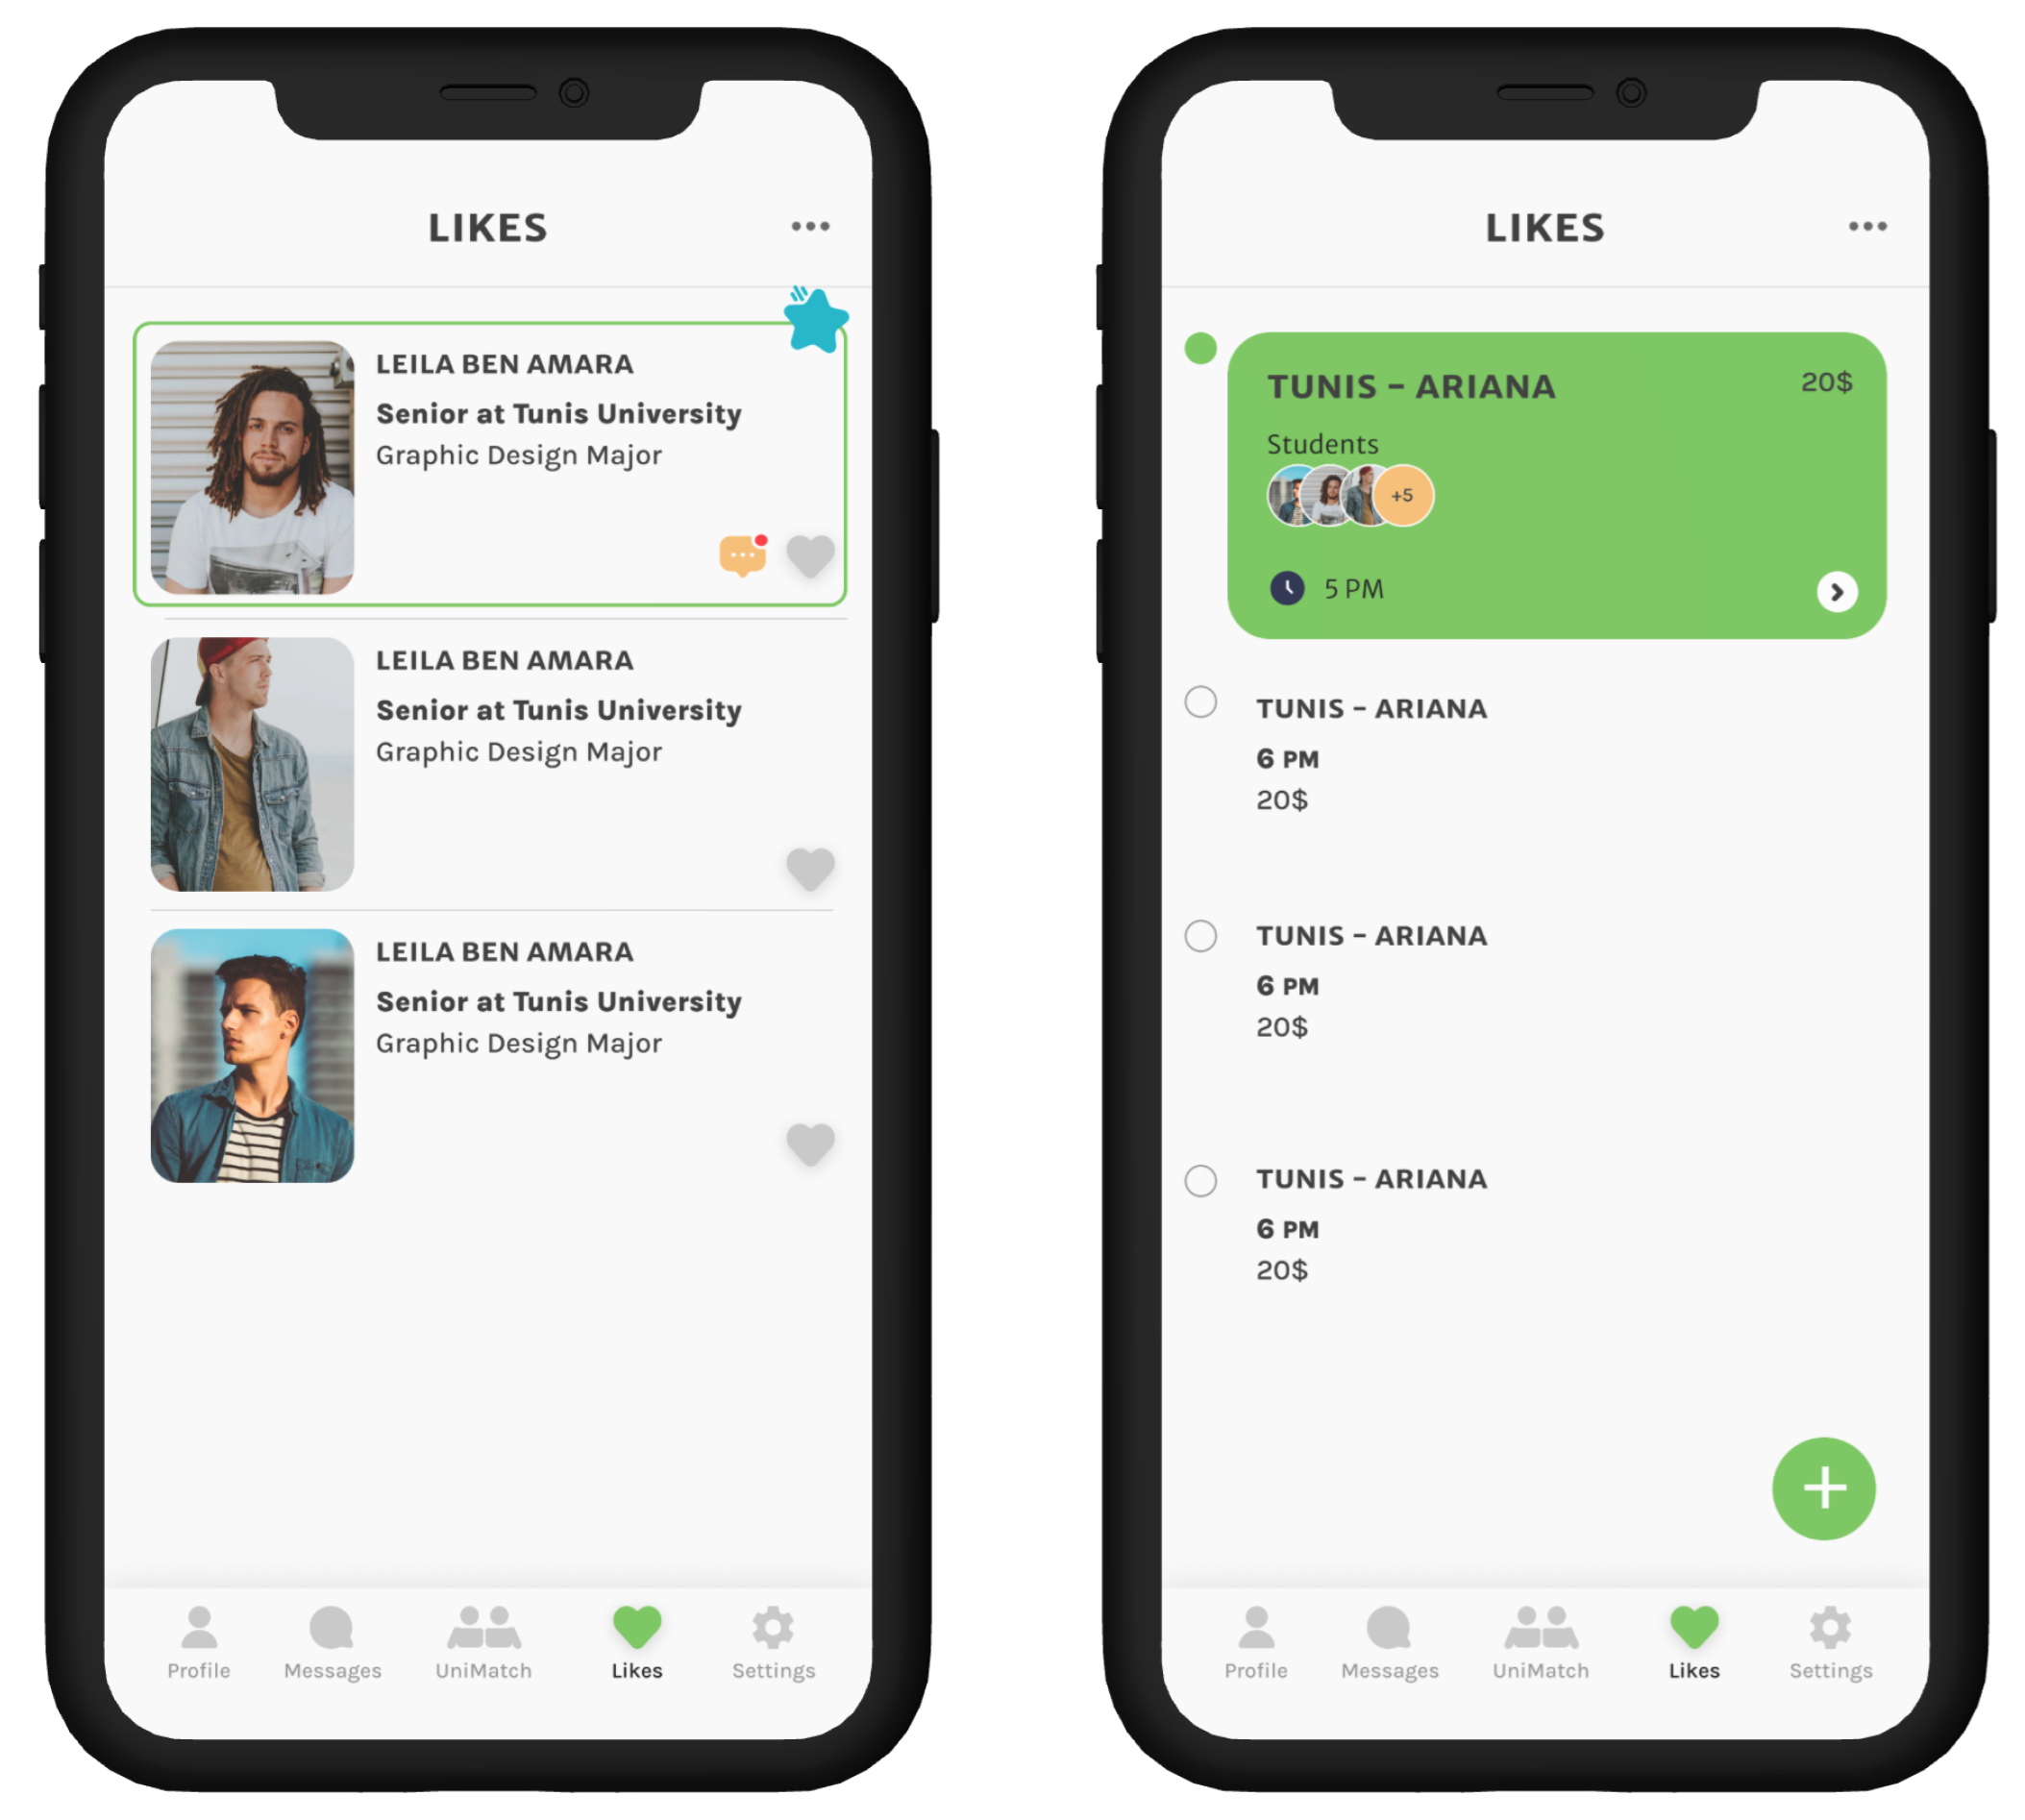
\includegraphics[scale=0.2]{ui/unicarpool offer managment.png}
            \caption{Uni-carpool offers management UI} 
            \label{fig: Uni-carpool offers management UI}
\end{figure}

\subsection{Messaging features}
As stated in the previous subsection, the owner can see who is interested in his offer. He then decides whether or not to decline or approve the sharing request. When he accepts a request, a new conversation is made which allows the sender of the request and the owner of the offer to interact. \\

Below, the direct message user interface is designed to enable users to communicate with one another.
\begin{figure}[H] 
            \centering
            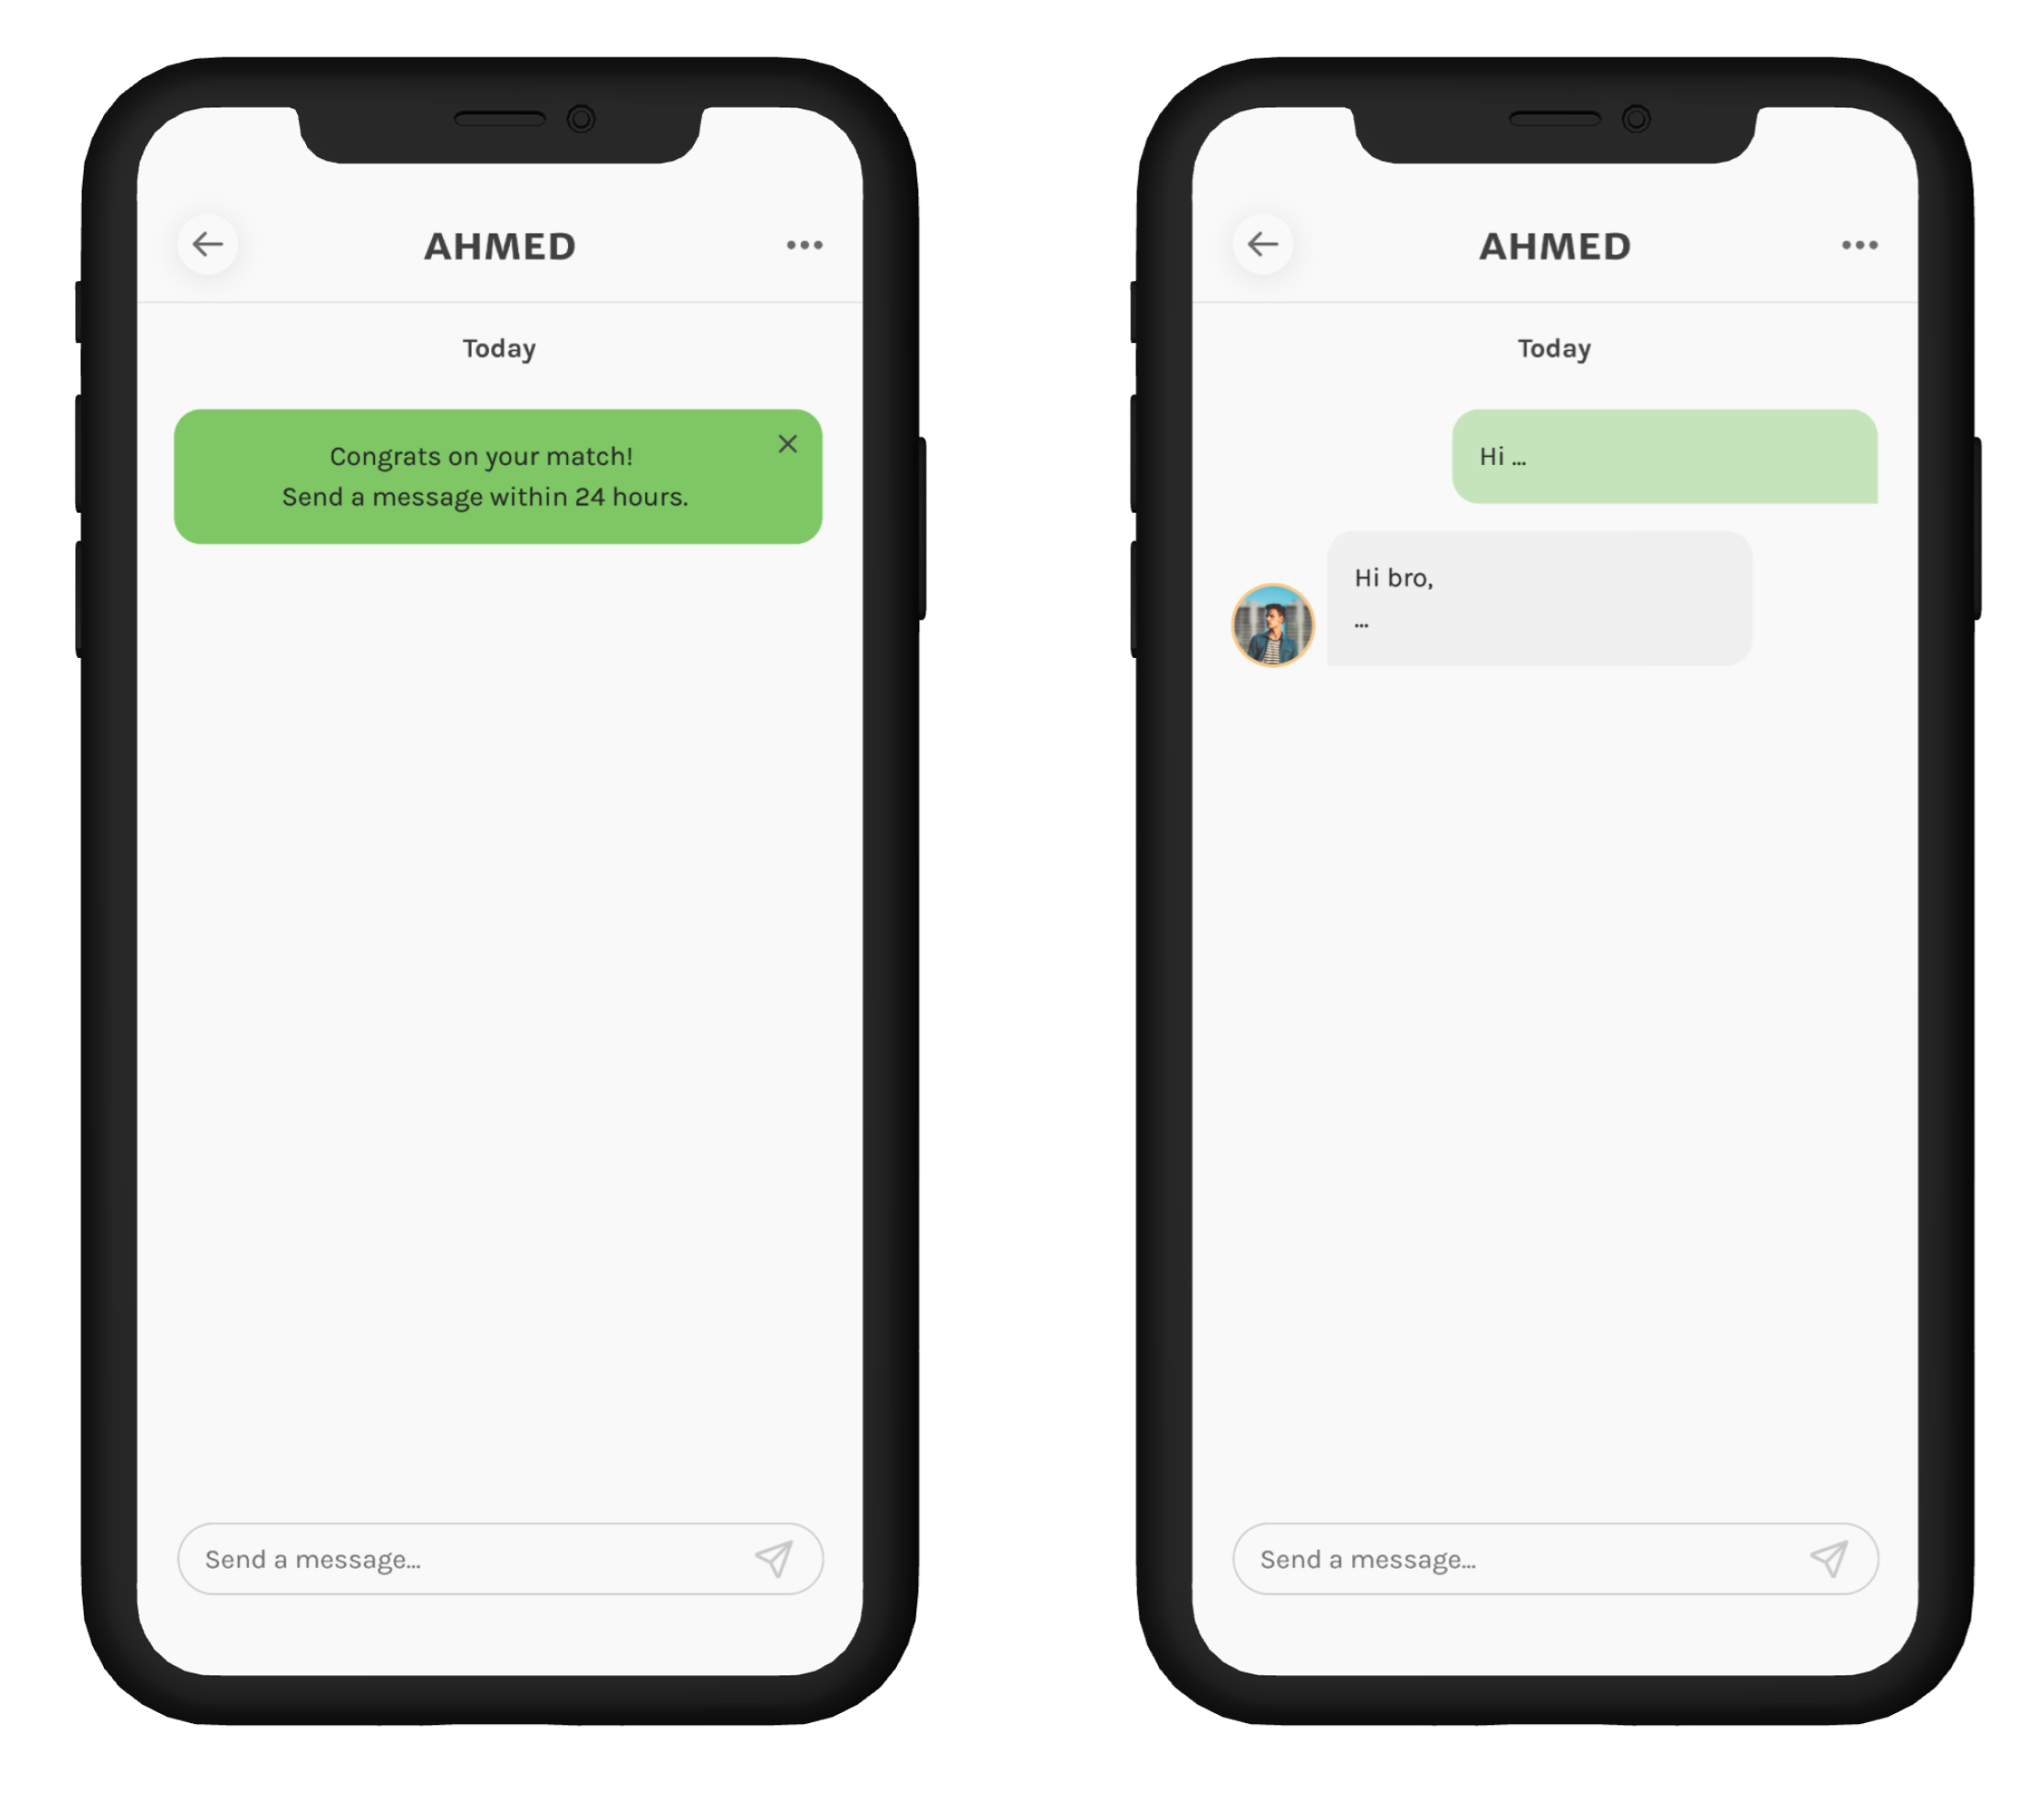
\includegraphics[scale=0.2]{ui/unicarpool messaging.png}
            \caption{Uni-carpool messages UI} 
            \label{fig: messages UI}
\end{figure}

\subsection{Filtering Management}
Last but not least, users can choose who they would like to see and have the capability of interacting with them due to a filter option. Users also have a possibility to regulate their potential network with a number of parameters: gender, field of study, university, interests, etc.\\
The following figure is the filtering interface:
\begin{figure}[H] 
            \centering
            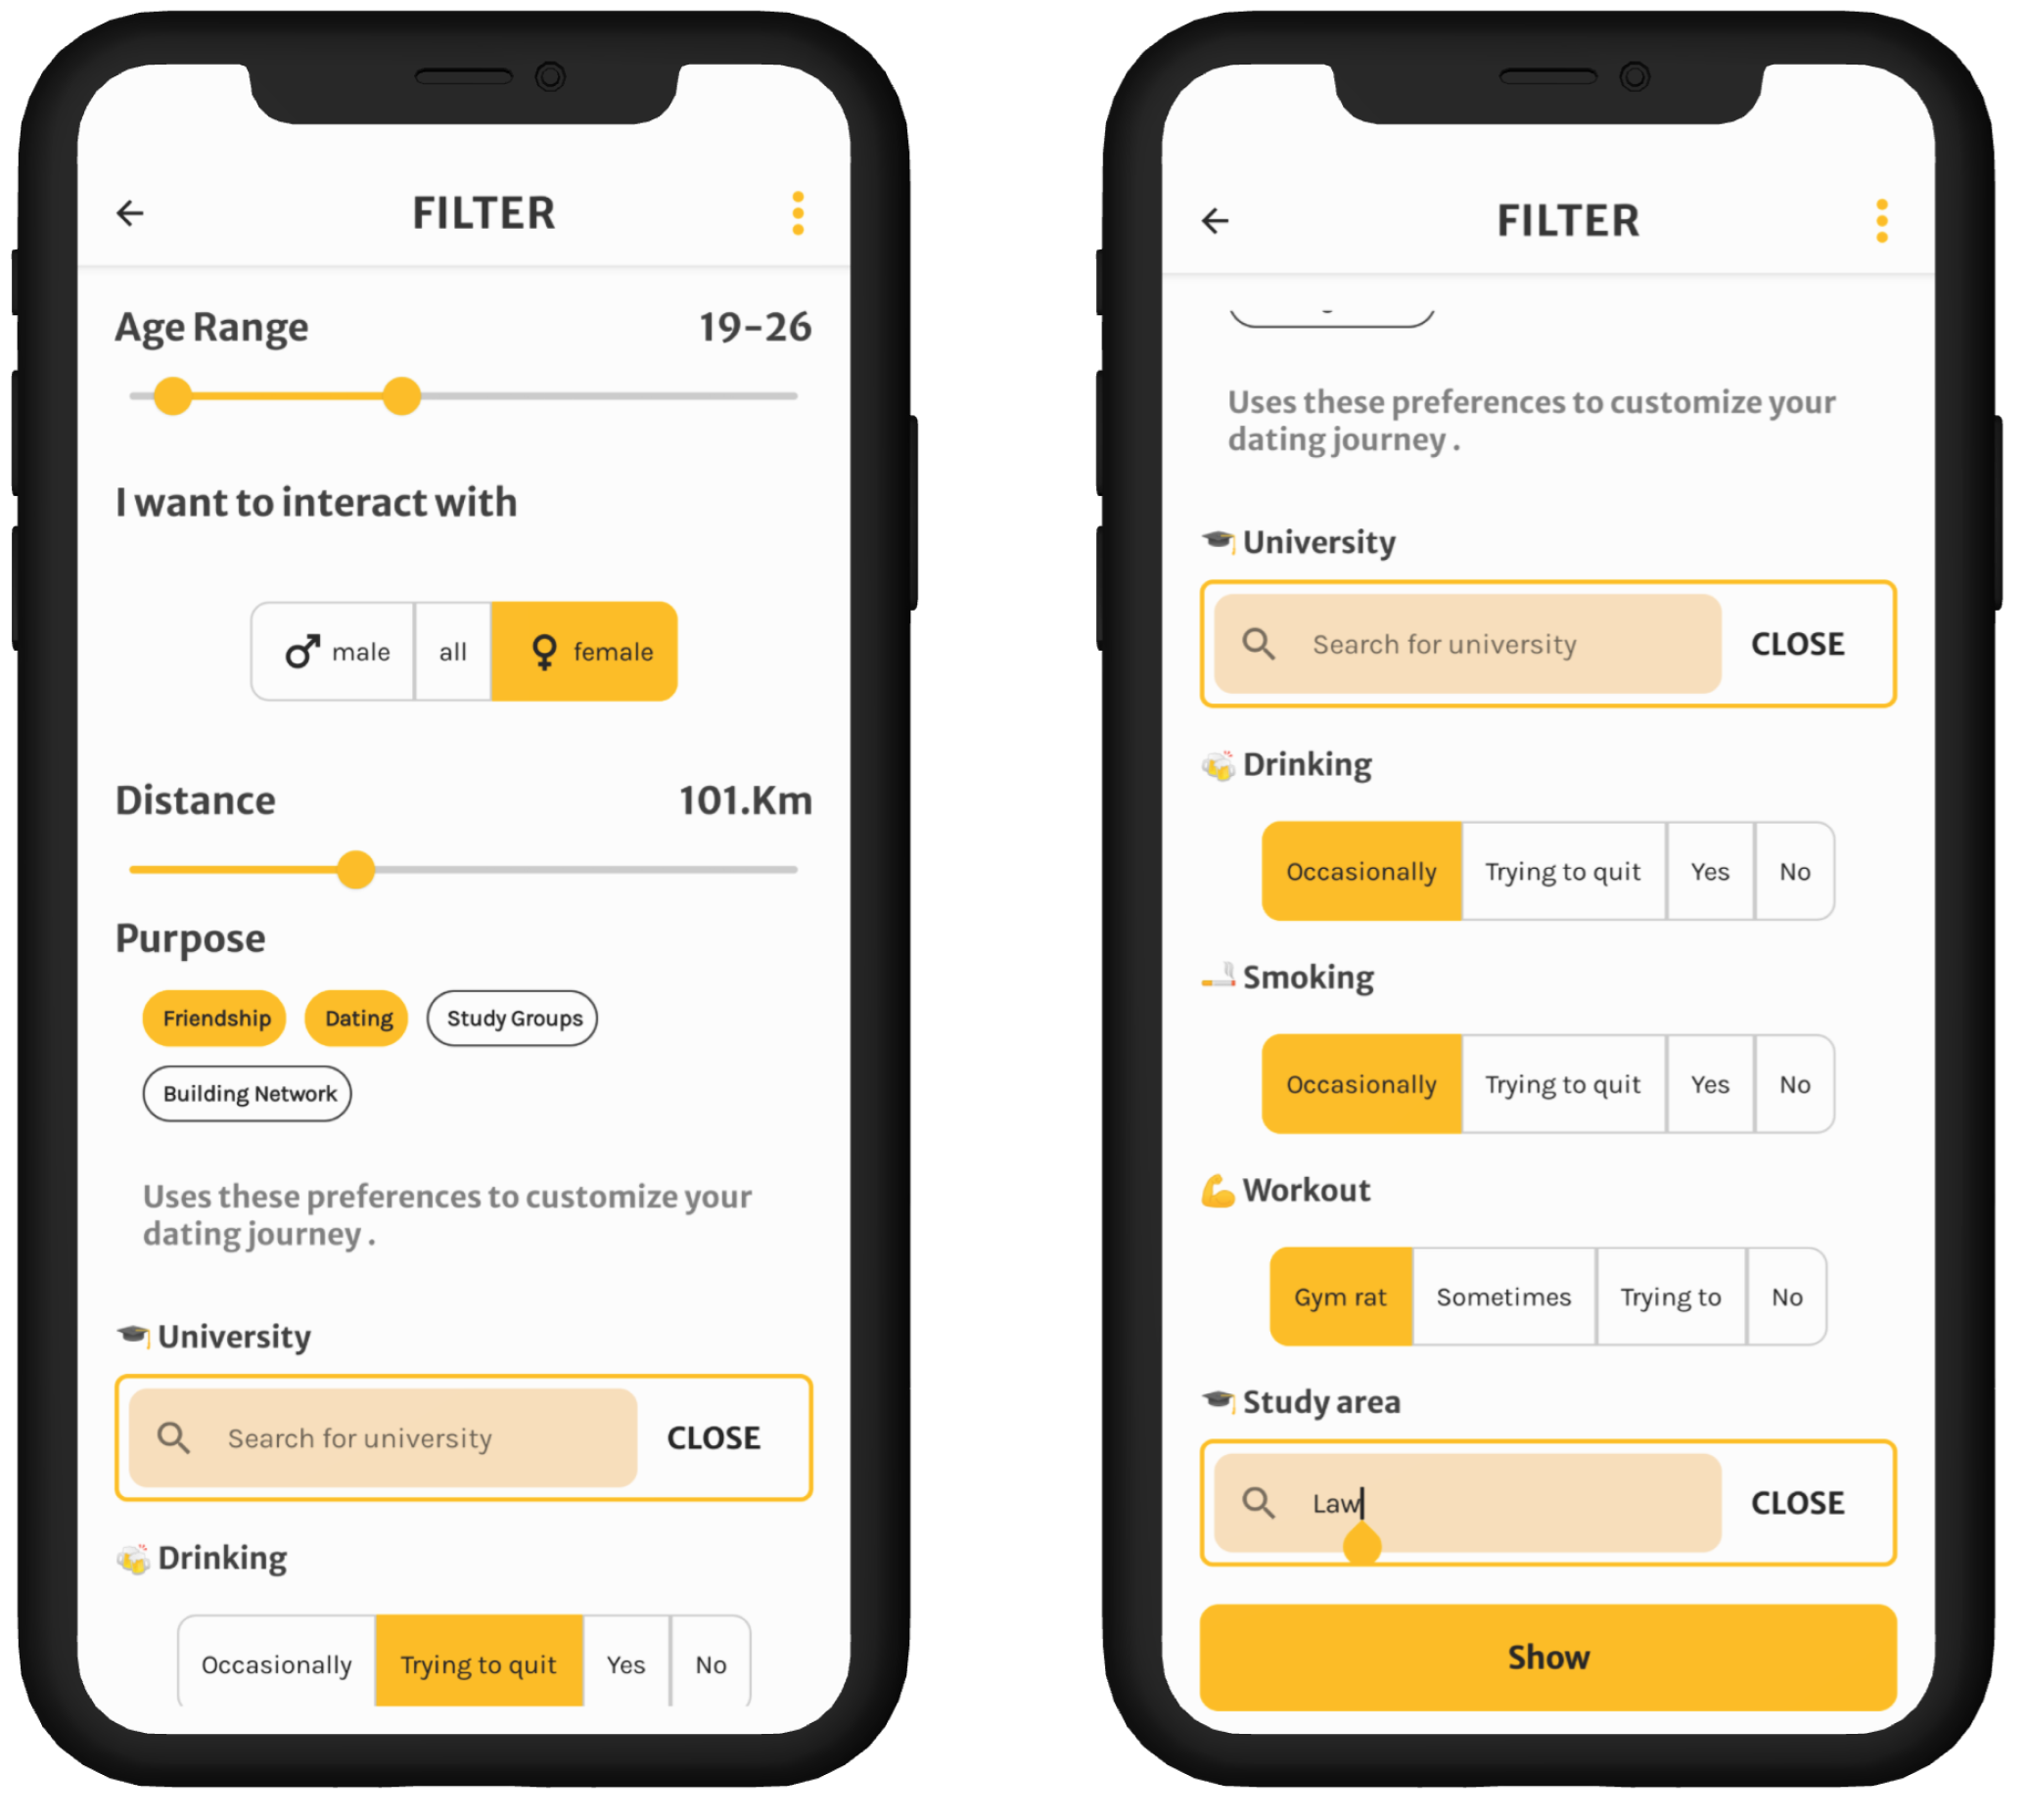
\includegraphics[scale=0.2]{filter ui.png}
            \caption{Feed Filter UI} 
            \label{fig: Feed Filter UI}
\end{figure}

\section*{Conclusion}
\addcontentsline{toc}{section}{Conclusion}
Sticking to the tradition of the chosen methodology, the first sprint introduced a design of the features that are complete for managing users and their authentication. The fact that it is possible to test and specifically these features in the subsequent sprints is the point that brings the team closer to the goal and the great immersive experience. 



%\chapter*{General conclusion}
\addcontentsline{toc}{chapter}{General conclusion}
The following report narrates the work accomplished during my final study internship at “Appaxis innovations” in the process of doing the national diploma in software engineering.
During my internship I was able to demonstrate all the knowledge and skills which have been introduced at the ESPRIT learning process and build the “Uni-world” application. This application has been designed with the objectives of overcoming and enhancing the student lives by providing the students with an environment to fund their network  and where they get the transportation benefits.
We start with the short brief, based on which we presented initial analysis of our work, demonstrating the general setting of our project, the issue we try to address, and the solution we offer. We then continued and explained the requirements analysis as well as Scrum management. We then elaborated the realization of the release 1, 2 and 3 explaining the functionality of the Sprints involved.
This project help me to enhance my technical skills, discover new technologies and work with tools like Kotlin, jetpack compose, and node .js .
I also learnt how to accurately determine the time needed by a certain task in a project to be completed.
I also succeeded in learning about and applying the Scrum methodology during the development phase and to be a part of forming a company’s growth as a leader and and as a member of a very hardworking and talented team. \\

Finally, in addition to the improvements suggested by our users, we are considering the integration of certain features such as :
\begin{enumerate}
    \item  Real-time account verification process.
    \item Home-sharing functionalities.
    \item Appointment scheduling function that include : selection of date and selection of place with maps.
    \item Community and discussion group creation
    \item Events creation

\end{enumerate}

%\bibliographystyle{abbrv}
%  classe les entrées par ordre alphabétique
\bibliographystyle{unsrt} 
% trie les entrées par ordre d'apparition dans le texte
\bibliography{references}

\end{document}
